% !TeX spellcheck = en_GB
%
\documentclass[handout]{beamer}
% \documentclass[presentation]{beamer}
\mode<presentation>{\usetheme{AMSCesenaPurpleAndGold}}
\setbeamertemplate{bibliography item}{\insertbiblabel}
\setbeamersize{description width=0.57cm}
%%%%%%%%%%%%%%%%%%%%%%%%%%%%%%%%%%%%%%%%%%%%%%%%%%%%%%%%%%%%%%%%%%%%%%%%%%%%%%%%
\usepackage{2p-kt-talk}
%%%%%%%%%%%%%%%%%%%%%%%%%%%%%%%%%%%%%%%%%%%%%%%%%%%%%%%%%%%%%%%%%%%%%%%%%%%%%%%%
\title[\twopkt]{
    \twopkt{}: A Kotlin Multi-Platform ecosystem for Symbolic AI
}
%
% \subtitle{Extended Abstract}
%
% same authors order of the presented paper
\author[Ciatto, Rizzato]{
    \emph{Giovanni Ciatto}$^{1}$ % empth the presenting author
    \and
    Lorenzo Rizzato$^{2}$
}
%
\institute[UniBo]{
    $^{1}$ Dipartimento di Informatica -- Scienza e Ingegneria (DISI)
    \\
    \textsc{Alma Mater Studiorum} -- Università di Bologna
    \\
    \texttt{
        giovanni.ciatto@unibo.it % emph the presenting author's email
    }
    \and
    $^{2}$\texttt{lorenzo.rizzato@studio.unibo.it}
}
%
\date[A.Y. 20-21]{
    Autonomous Systems Course, A.Y. 2020-2021
}
%%%%%%%%%%%%%%%%%%%%%%%%%%%%%%%%%%%%%%%%%%%%%%%%%%%%%%%%%%%%%%%%%%%%%%%%%%%%%%%%
\AtBeginSection[]{
    \begin{frame}<beamer>[shrink,noframenumbering]\frametitle{Next in Line\ldots}
        \mbox{~}
        \tableofcontents[sectionstyle=show/shaded,subsectionstyle=hide,subsubsectionstyle=hide]
        \mbox{~}
    \end{frame}
}
\AtBeginSubsection[]{
    \begin{frame}<beamer>[shrink,noframenumbering]\frametitle{Focus on\ldots}
        \mbox{~}
        \tableofcontents[sectionstyle=show/shaded,subsectionstyle=show/shaded,subsubsectionstyle=hide]%[currentsection,currentsubsection,sectionstyle=shaded,subsectionstyle=shaded,subsubsectionstyle=hide]
        \mbox{~}
    \end{frame}
}
%%%%%%%%%%%%%%%%%%%%%%%%%%%%%%%%%%%%%%%%%%%%%%%%%%%%%%%%%%%%%%%%%%%%%%%%%%%%%%%%
\begin{document}
%%%%%%%%%%%%%%%%%%%%%%%%%%%%%%%%%%%%%%%%%%%%%%%%%%%%%%%%%%%%%%%%%%%%%%%%%%%%%%%%

%\\\\\\\\\\\\\\\\\\\\\
\frame{\titlepage}
%\\\\\\\\\\\\\\\\\\\\\

\begin{frame}<beamer>[shrink,noframenumbering]\frametitle{Outline}
    \mbox{~}
    \tableofcontents
    \mbox{~}
\end{frame}

\section{Historical Perspective}

\subsection{Prolog History}

\begin{frame}{Implementations of Prolog -- Chronological Perspective}
    % !TEX root = 2p-kt-talk.tex
\begin{figure}[h]\centering
    \tiny
    \catcode`\@=11
    \def\chron@selectmonth#1{\ifcase#1\or January\or February\or
    March\or April\or May\or June\or
    July\or August\or September\or
    October\or November\or December\fi}
    \startchronology[startyear=1972,startdate=false,stopdate=false,stopyear=1995]
    \chronoevent[markdepth=-20pt]{1972}{1st Prolog}
    \chronoevent{1973}{Final Marseille's Prolog}
    \chronoevent[markdepth=-20pt]{1977}{Prolog II}
    \chronoevent[markdepth=40pt]{1977}{DEC-10 Prolog}
    \chronoevent[markdepth=-20pt]{1982}{C-Prolog}
    \chronoevent[markdepth=10pt]{1983}{\textbf{\emph{(The WAM)}}}
    \chronoevent[markdepth=-50pt]{1984}{Quintus}
    \chronoevent[markdepth=-20pt]{1986}{SICStus~ ~}
    \chronoevent[markdepth=40pt]{1986}{\&-Prolog/Ciao}
    \chronoevent[markdepth=-20pt]{1988}{~CLP(R)} % Could be in 87 also, but does not fit
    \chronoevent[markdepth=-50pt]{1987}{SWI-Prolog}
    \chronoevent[markdepth=10pt]{1988}{SB-Prolog}
    \chronoevent[markdepth=-50pt]{1990}{\eclipse{}}
    \chronoevent[markdepth=40pt]{1991}{BinProlog}
    \chronoevent[markdepth=-20pt]{1993}{XSB}
    \chronoevent[markdepth=5pt]{1993}{wamcc}
    \chronoevent[markdepth=40pt]{1994}{B-Prolog}
    \chronoevent[markdepth=15pt]{1995}{GNU Prolog}
    \chronoevent[markdepth=-50pt]{1995}{\textbf{\emph{(ISO Prolog)}}}
    % SICStus, YAP somewhat unclear
    % Cannot fit MU-Prolog...
    \stopchronology
    % \caption{Timeline of Early Prolog-Related Systems (up to the ISO Standard)}%
    \label{fig:timeline}
\end{figure}
\end{frame}

\begin{frame}{Implementations of Prolog -- Familiy Tree}
    % !TEX root = 2p-kt-talk.tex
\begin{figure}
\tikzstyle{inactive}=[rectangle, draw=black, rounded corners, fill=gray!50, drop shadow,
        text centered, anchor=north, text=black]
\tikzstyle{active}=[rectangle, draw=black, rounded corners, fill=white, drop shadow,
        text centered, anchor=north, text=black]
\tikzstyle{myarrow}=[->, >=open triangle 90, thick]
\tikzstyle{line}=[-, thick]

\pgfdeclarelayer{background}
\pgfdeclarelayer{foreground}
\pgfsetlayers{background,main,foreground}
\usetikzlibrary{positioning}
\begin{adjustbox}{width=.8\textwidth}    
    \begin{tikzpicture}[node distance=.6cm]
    % \node (Prolog0) [inactive, rectangle split, rectangle split parts=2]
    %     {
    %         \textbf{Prolog 0}
    %         \nodepart{second}{\scriptsize first Prolog System}
    %     };
    \node (Prolog1) [inactive, rectangle split, rectangle split parts=2]
        {
            \textbf{Prolog 0 \& I}
            \nodepart{second}{\scriptsize negation as failure}
        };
    % \draw[-Stealth] (Prolog0.south) -- (Prolog1.north) ;

    \node (Prolog2) [inactive, rectangle split, rectangle split parts=2, below=of Prolog1]
        {
            \textbf{Prolog II}
            \nodepart{second}{\scriptsize cyclic structures}
        };
    \draw[-Stealth] (Prolog1.south) -- (Prolog2.north) ;

    \node (Prolog3) [inactive, rectangle split, rectangle split parts=2, below=of Prolog2]
        {
            \textbf{Prolog III}
            \nodepart{second}{\scriptsize constraints}
        };
    \draw[-Stealth] (Prolog2.south) -- (Prolog3.north) ;

    \node (Prolog4) [inactive,
      % rectangle split, rectangle split  parts=2,
    below=of Prolog3]
        {
            \textbf{Prolog IV}
            % \nodepart{second}{\scriptsize constraints}
        };
    \draw[-Stealth] (Prolog3.south) -- (Prolog4.north) ;

    \node (DEC10) [inactive, rectangle split, rectangle split parts=2, right=of Prolog1, yshift=-3mm]
        {
            \textbf{DEC-10 Prolog}
            \nodepart{second}{\scriptsize compiled, de facto standard}
        };
    \draw[-Stealth] (Prolog1.east) -- (DEC10.west);

    \node (CProlog) [inactive, rectangle split, rectangle split parts=2, right=of DEC10, yshift=-2mm]
        {
            \textbf{C-Prolog}
            \nodepart{second}{\scriptsize interpreted, portable}
        };
    \draw[-Stealth] (DEC10.east) -- (CProlog.west);

    \node (WAM) [inactive, rectangle split, rectangle split parts=2, below=of DEC10, yshift=1mm]
        {
            \textbf{The WAM} % Warren Abstract Machine (WAM)
            \nodepart{second}{\scriptsize compiled, portable}
        };
    \draw[-Stealth] (DEC10.south) -- (WAM.north);
    \node (Quintus) [inactive, rectangle split, rectangle split parts=2, below=of WAM, yshift=2mm]
        {
            \textbf{Quintus}
            \nodepart{second}{\scriptsize commercial, de-facto standard}
        };
    \draw[-Stealth] (WAM.south) -- (Quintus.north);

    \node (SICStus) [active, rectangle split, rectangle split parts=2, below=of Quintus, yshift=3mm]
        {
            \textbf{SICStus}
            \nodepart{second}{\scriptsize commercial support, JIT}
        };
    \draw[-Stealth] (Quintus.south) -- (SICStus.north);

    \node (BIM) [inactive, rectangle split, rectangle split parts=2, right=of Quintus, xshift=6mm, yshift=-4mm]
        {
            \textbf{BIM} % -Prolog
            \nodepart{second}{\scriptsize commercial, native}
        };
    \draw[-Stealth] (WAM.east) -| (BIM.north);

    \node (Ciao) [active, rectangle split, rectangle split parts=2, below=of SICStus, yshift=3mm]
        {
            \textbf{\&-Prolog/Ciao}
            \nodepart{second}{\scriptsize parallel, assertions}
        };
    \draw[-Stealth] (SICStus.south) -- (Ciao.north);

    \node (SWI) [active, rectangle split, rectangle split parts=2, right=of Ciao]
        {
            \textbf{\ SWI\ } % SWI-Prolog
            \nodepart{second}{\scriptsize libraries}
        };
    \draw[-Stealth] (Quintus.south east) -- (SWI.north);

    \node (YAP) [active, rectangle split, rectangle split parts=2, right=of SWI]
        {
            \textbf{YAP} % -Prolog
            \nodepart{second}{\scriptsize indexing}
        };
    \draw[-Stealth] (Quintus.east) -- (YAP.north west);

    \node (SB) [inactive,
    % rectangle split, rectangle split parts=2,
    right=of YAP]
        {
            \textbf{SB-Prolog}
            \nodepart{second}
        };
    \draw[-Stealth] (WAM.east) -| (SB.north);

    \node (XSB) [active, rectangle split, rectangle split parts=2, below=of SB]
        {
            \textbf{XSB}
            \nodepart{second}{\scriptsize tabling}
        };
    \draw[-Stealth] (SB.south) -- (XSB.north);

    \node (GNU) [active, rectangle split, rectangle split parts=2, right=of XSB]
        {
            \textbf{GNU} % -Prolog
            \nodepart{second}{\scriptsize fd/indexicals}
        };
    \draw[-Stealth] (WAM.east) -| (GNU.north);

    \node (OtherW) [active, right=of GNU, xshift=-2mm]
        {
            \textbf{\ \ \ldots\ \ }
        };

    \node (BProlog) [active, rectangle split, rectangle split parts=2, left=of XSB]
        {
            \textbf{B-Prolog}
            \nodepart{second}{\tiny TOAM}
        };
    \draw[-Stealth] (SB.south west) -- (BProlog.north east);

    \node (Bin) [active, rectangle split, rectangle split parts=2, left=of BProlog, xshift=3mm]
        {
            \textbf{BinProlog}
            \nodepart{second}{\scriptsize binarization}
        };

    \node (tuProlog) [active, rectangle split, rectangle split parts=2, left=of Bin, xshift=3mm]
        {
            \textbf{tuProlog}
            \nodepart{second}{\scriptsize jvm, interop.} % interoperability
        };

    \node (OtherNW) [active, below=of BProlog, xshift=3mm, yshift=4mm]
        {
            \textbf{\ \ \ldots\ \ } 
        };

    \node (Marseille1) [below= 2mm of Prolog4]
        {
            \textbf{Marseille}
        };
    \node (Marseille2) [below= -1mm of Marseille1]
        {
            \textbf{Prolog-line}
        };

    \node (WAM-comment2) [right=of Quintus, xshift=-2mm, yshift=4mm]
        {
            \textbf{Prologs}
        };
    \node (WAM-comment1) [above=0mm of WAM-comment2]
        {
            \textbf{WAM-based}
        };
    % \node (WAM-comment) [below= 1mm of GNU, align=right,xshift=-6mm]
    %     {
    %         \textbf{WAM-based Prologs}
    %     };

    \node (NWAM-comment) [below=1mm of tuProlog,align=right,xshift=5mm]
        {
            \textbf{WAM alternatives}
        };

        \begin{pgfonlayer}{background}
        \path (Prolog1.west |- Prolog1.north)+(-0.2,0.2) node (a) {};
        \path (Marseille2.east |- Marseille2.south)+(+0.3,0) node (c) {};
        \path[fill=gray!5,rounded corners, draw=black!50, dashed]
              (a) rectangle (c);

        \path (Quintus.west |- WAM.north)+(-0.2,0.2) node (wam-a) {};
        \path (OtherW.east |- GNU.south)+(+0.2,-0.2) node (wam-c) {};
        \path[fill=gray!5,rounded corners, draw=black!50, dashed]
              (wam-a) rectangle (wam-c);

        \path (tuProlog.west |- tuProlog.north)+(-0.2,0.2) node (nwam-a) {};
        \path (BProlog.east |- NWAM-comment.south)+(+0.3,-0.1) node (nwam-c) {};
        \path[fill=gray!5,rounded corners, draw=black!50, dashed]
              (nwam-a) rectangle (nwam-c);
        \end{pgfonlayer}
    \end{tikzpicture}
\end{adjustbox}
\caption{Prolog implementations in perspective. Notice the pivotal role of the WAM \cite{Warren1983}}
\end{figure}

\end{frame}

\begin{frame}[allowframebreaks]{Implementations of Prolog -- Features}
    % !TEX root = 2p-kt-talk.tex
\centering

\begin{adjustbox}{width=.8\textwidth} 
    \begin{tabular}{|l|ccccccc|}
        \hline
        System            & Open Source  & Modules  & Tabling  & Parallelism  & CLP            & CHR      & Global Variables  \hfill \\
        \hline\hline
        B-Prolog          & \xmark       & \xmark   & \cmark   & \xmark       & FD, B, Set     & (\cmark) & \cmark \\
        Ciao              & \cmark       & \cmark   & \cmark   & \cmark       & Q, R, FD       & \cmark   & \cmark \\
        ECLiPSe           & \cmark       & \cmark   & \xmark   & \cmark       & FD, Q, R, Set  & \cmark   & \cmark \\
        GNU Prolog        & \cmark       & \xmark   & \xmark   & \xmark       & FD, B          & \xmark   & \cmark \\
        Jekejeke          & \xmark       & \cmark   & \xmark   & \cmark       & FD, B          & \cmark   & \xmark \\
        JIProlog          & \cmark       & \cmark   & \xmark   & \xmark       & \xmark         & \xmark   & \xmark \\
        SWI               & \cmark       & \cmark   & \cmark   & \cmark       & FD, B, Q, R    & \cmark   & \cmark \\
        SICStus           & \xmark       & \cmark   & \xmark   & \xmark       & FD, B, Q, R    & \cmark   & \xmark \\
        tauProlog         & \cmark       & \cmark   & \xmark   & \xmark       & \xmark         & \xmark   & \xmark \\
        tuProlog          & \cmark       & \xmark   & \xmark   & \cmark       & \xmark         & \xmark   & \xmark \\
        XSB               & \cmark       & \cmark   & \cmark   & \cmark       & R              & \cmark   & \xmark \\
        YAP               & \cmark       & \cmark   & \cmark   & \xmark       & \cmark         & \cmark   & \cmark \\
        \hline
    \end{tabular}
\end{adjustbox}

\framebreak

\begin{adjustbox}{width=.8\textwidth} 
    \begin{tabular}{|l|cccccc|}
        \hline
        System            &  Indexing       & Type / Mode & Co-Routines  & Testing      & Debugger          & Mutable Terms \hfill\\
        \hline\hline
        B-Prolog          &  N-FA           & \xmark      & (\cmark)     & \xmark       & trace             & \xmark \\
        Ciao              &  FA, MA         & \cmark      & \cmark       & \cmark       & trace / source    & \cmark \\
        ECLiPSe           &  most suitable  & \xmark      & \cmark       & \cmark       & trace             & \xmark \\
        GNU Prolog        &  FA             & \xmark      & \xmark       & \xmark       & trace             & \cmark \\
        Jekejeke          &  FA, N-FA, MA   & \xmark      & \cmark       & \xmark       & spy               & \xmark \\
        JIProlog          &  undocumented   & \xmark      & \xmark       & \xmark       & trace             & \xmark \\
        SWI               &  JIT, MA, deep  & \xmark      & \cmark       & \cmark       & trace / graphical & \cmark \\
        SICStus           &  FA             & \xmark      & \cmark       & \cmark       & trace / source    & \cmark \\
        tauProlog         &  undocumented   & \xmark      & \xmark       & \xmark       & \xmark            & \xmark \\
        tuProlog          &  FA             & \xmark      & \xmark       & \xmark       & spy               & \xmark \\
        XSB               &  all, trie      & \xmark      & \cmark       & \xmark       & trace             & \xmark \\
        YAP               &  FA,MA,jit      & \xmark      & \xmark       & \xmark       & trace             & \xmark \\
        \hline
    \end{tabular}
\end{adjustbox}

\framebreak

\begin{adjustbox}{width=.5\textwidth} 
    \begin{tabular}{|l|cc|}
        \hline
        System            & FLI                  & Non-Standard Data Types     \\ 
        \hline\hline
        B-Prolog          & C, Java              & arrays, sets, hashtables               \\
        Ciao              & C, Java, Python, JS  & \xmark\\
        ECLiPSe           & C, Java, Python, PHP & arrays, strings,         \\
        Jekejeke          & Java                 & arrays          \\
        JIProlog          & Java                 & \xmark \\
        GNU Prolog        & C, Java, PHP         & arrays          \\
        tauProlog         & JavaScript           & \xmark          \\
        tuProlog          & Java, .NET, Android, iOS           & arrays          \\
        SWI               & C, C++, Java         & dicts, strings \\
        SICStus           & C, Java, .NET, Tcl/Tk & \xmark              \\
        XSB               & C, Java, PERL        & \xmark                \\
        YAP               & C, Python, R         & \xmark                \\
        \hline
    \end{tabular}
\end{adjustbox}


\end{frame}

\subsection{\tuprolog{} History}

\begin{frame}[allowframebreaks]{\tuprolog{} History}
\begin{block}{Foundational features and ideas}
	\begin{itemize}
		\item light-weight Prolog system for \alert{distributed} applications and infrastructures \ccite{tuprolog-padl01}
		\item intentionally designed around a \alert{minimal core}
		\item to be either statically or dynamically \emph{configured} by loading/unloading \alert{libraries} of predicates
		\item \tuprolog{} natively supports \alert{multi-paradigm programming} \ccite{tuprolog-scp57}, providing a clean, seamless integration model between Prolog and mainstream object-oriented languages
	\end{itemize}
\end{block}

\framebreak

\begin{itemize}
	\item first release lightweight Prolog solver written in Java \ccite{tuprolog-padl01}
	\begin{itemize}
		\item state of the art advancements: OOP-interoperable, and SM-based \ccite{weblp-ia5}
	\end{itemize}
	\item extended along many research directions
	\begin{description}
		\item[LPaaS] micro-intelligence vision (lightweight logic solvers running on most devices) for IoT and Cloud/Edge computing \ccite{lpaas-tplp18}
		\item[TuSoW] bringing tuple-based coordination at the edge \ccite{tusow-icccn2019}
	\end{description}
	\item foundation of many research projects
	\begin{description}
		\item[TuCSoN / ReSpecT] coordination model for Internet applications based on network-aware and mobile agents \ccite{tucson-jaamas2} by means of reactions to communication events \ccite{respect-scp41}
		\item[MoK] self-organising knowledge-oriented model based on biochemical tuple space \ccite{mok-idc2012}
		\item[Arg2P] defeasible reasoning and argumentation tool \ccite{arg2p-cilc2020}
	\end{description}
\end{itemize}

\framebreak

\begin{itemize}
	\item[$\rightarrow$] legacy code: making it Prolog-constrained and hard to maintain
	\item[$\rightarrow$] complete re-design and re-write as Kotlin MPP
	\begin{itemize}
		\item[$\Rightarrow$]  widening the scope to whole LP rather than Prolog alone
	\end{itemize}
\end{itemize}

\end{frame}

\section{Motivation}

\begin{frame}{Why \twopkt{}}
    \begin{itemize}
        \item Building an open an extensible ecosystem\ldots
        \vfill
        \item \ldots supporting \alert{multiple logics} (e.g. FOL, DL, TL, BDI, etc)
        %
        \begin{itemize}
            \item via as many \alert{inference rules} as possible (e.g. deduction, abduction, induction)
            %
            \begin{itemize}
                \item implemented, in turn, via multiple \alert{resolution strategies} (e.g. SLDNF, IFF, Probabilistic, etc.)
            \end{itemize}
        \end{itemize}
        \vfill
        \item Making each aspect of LP individually usable \emph{per se}
        \vfill
        \item Reaching widest possible platform support
        \vfill
        \item Blending LP with OOP and FP
        \vfill
        \item Bridging symbolic and sub-symbolic AI
    \end{itemize}
\end{frame}

\begin{frame}{Which features of LP}
    \begin{enumerate}
        \item Knowledge representation: \alert{terms}, and \alert{clauses}
        \vfill
        \item \alert{Unification}, based on \cite{MartelliMontanari1982} but possibly customisable
        \vfill
        \item Clauses \alert{indexing} and in-memory \alert{storage} facilities for \alert{knowledge bases}
        \vfill
        \item Prolog-like syntax \alert{parsing} \& \alert{formatting}
        \vfill
        \item \alert{Serialization} / \alert{deserialization} of terms, clauses, and knowledge bases
        \vfill
        \item Generic \alert{resolution} API, possibly customisable via \alert{pluggable features}
        \vfill
        \item \alert{SLD NF} (Prolog-like) resolution streategy \cite{Robinson65SLD,Clark77}
        \vfill
        \item Support for other resolution strategies
        \vfill
        \item Common \alert{UI} facilities
        \vfill
        \item[\vdots]
    \end{enumerate}
\end{frame}

\begin{frame}{Why Kotlin}
    \begin{itemize}
        \item Multi-platform support:
        %
        \begin{itemize}
            \item JVM (Win + Linux + Mac)
            \item JS (Web, both browser and server side)
            \item Android
            \item Native?
            \item iOS?
        \end{itemize}

        \vfill

        \item Good platform-specific interoperability
        %
        \begin{itemize}
            \item Kotlin libraries can easily be exploited in bare Java projects
            \item Kotlin libraries can be exploited in bare JavaScript projects
        \end{itemize}

        \vfill

        \item Clean and practical framework and tool-kit available
    \end{itemize}
\end{frame}

\section{Overview of the Project}

\begin{frame}[allowframebreaks]{Project Map}
    \begin{itemize}
        \item \twopkt{} is an ecosystem of \alert{modules}
        %
        \begin{itemize}
            \item denoted by Gradle's notation: \module{moduleName}
        \end{itemize}

        \medskip

        \item Modules are \alert{loosely-coupled}, yet incrementally inter-dependent
        %
        \begin{itemize}
            \item[$\rightarrow$] \alert{onion-like} architectural design
        \end{itemize}

        \medskip

        \item Modules are compilation and \alert{deployment units}
        %
        \begin{itemize}
            \item 1 module $\leftrightarrow$ 1 jar, on the JVM
        \end{itemize}

        \medskip

        \item Using a module as a dependecy $\implies$ importing \alert{all} its dependencies
    \end{itemize}

    \framebreak

    \begin{center}
        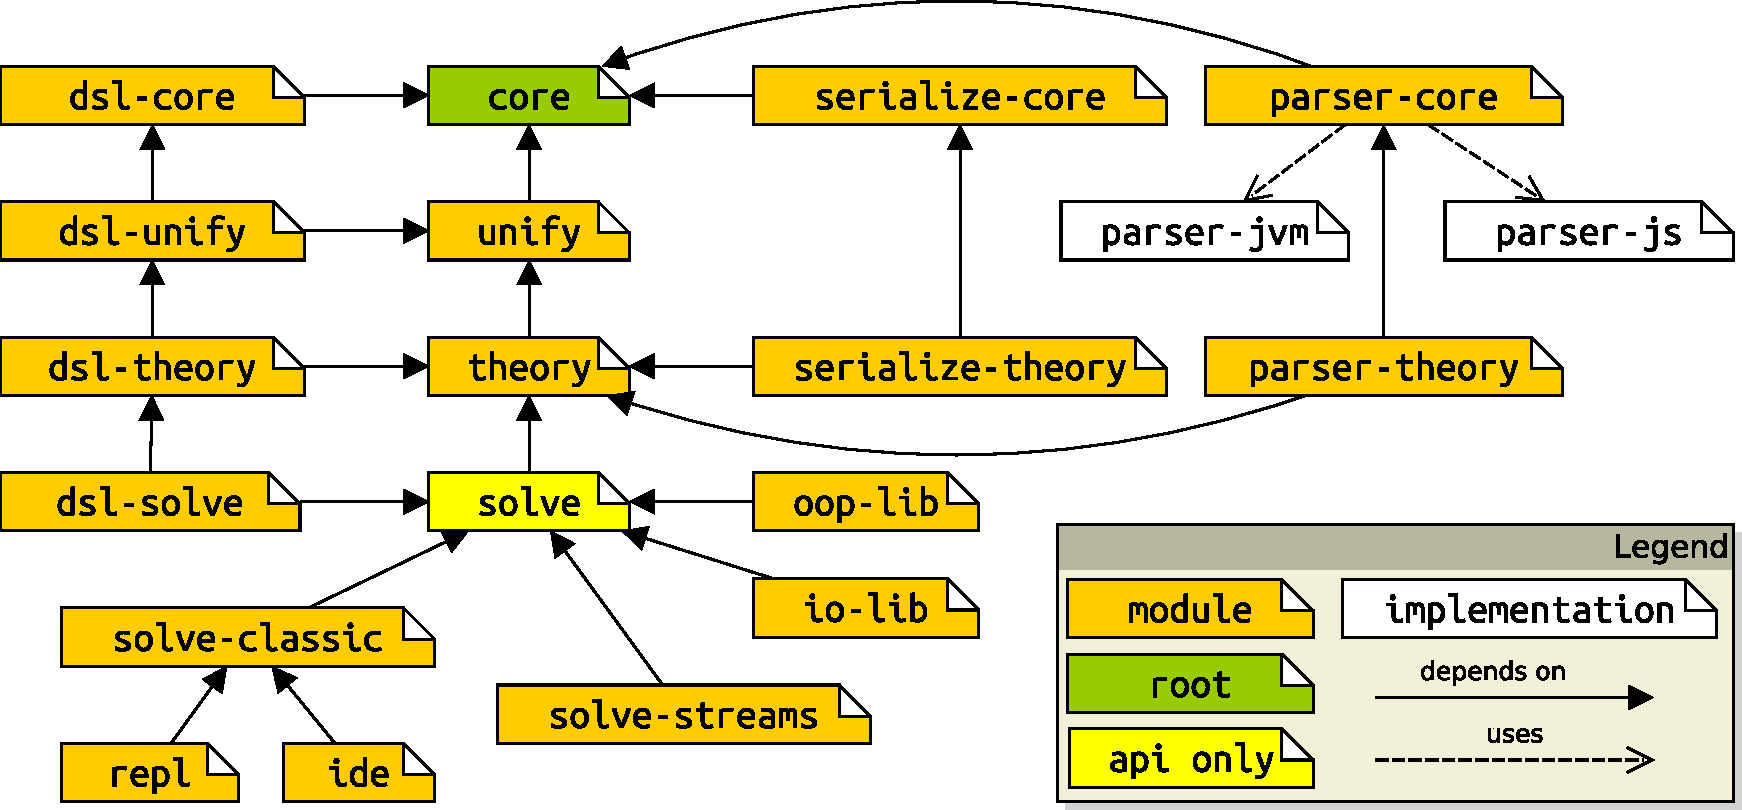
\includegraphics[width=\linewidth]{img/project-map.pdf}
    \end{center}

    \framebreak

    \begin{description}
        \item[\module{core}] provides \alert{knowledge representations} facilities \& common features
        %
        \begin{itemize}\small
            \item[eg] terms, clauses, substitutions, operators, term formatting, basic exceptions, etc.
        \end{itemize}

        \medskip

        \item[\module{unify}] provides support for \alert{logic unification}
        %
        \begin{itemize}\small
            \item[eg] customisable notion of unificator based on \cite{MartelliMontanari1982}
        \end{itemize}

        \medskip

        \item[\module{theory}] provides support in-memory \alert{storage \& indexing} of clauses
        %
        \begin{itemize}\small
            \item[eg] mutable/immutable and ordered/unordered \alert{collections of clauses} + \alert{logic theories}
        \end{itemize}

        \medskip

        \item[\module{solve}] provides generic support for \alert{resolution-related} stuff
        %
        \begin{itemize}\small
            \item[!] agnostic w.r.t. inference procedures \& resolution strategy
            \item[eg] solvers, solutions, libraries, errors, flags, channels, etc.
        \end{itemize}

        \framebreak

        \item[\module{solve-*}] provide specific implementation for inference procedures \& \alert{resolution} strategy
        %
        \begin{description}\small
            \item[\module{solve-classic}] SLD NF (Prolog-like) resolution \cite{Robinson65SLD,Clark77} based on Piancastelli's state machine \cite{tuprolog-sac08} (\alert{Prolog ISO \cite{prologISO-pt1} Compliant})
            \item[\module{solve-streams}] SLD NF (Prolog-like) resolution \cite{Robinson65SLD,Clark77} based on Enrico Siboni's master thesis and on \cite{Carlsson84}
        \end{description}

        \medskip

        \item[\module{parser-*}] supports \alert{parsing} of terms and clauses in Prolog syntax
        %
        \begin{description}\small
            \item[\module{parser-core}] supports parsing terms
            \item[\module{parser-theory}] supports parsing knowledge bases and streams of clauses
            \item[\module{parser-jvm/js}] platform-specific implementations, based on ANTLR \cite{Parr2013} \hint{(not to be used directly!)}
        \end{description}

        \framebreak

        \item[\module{serialization-*}] support \alert{(de)serialization} of terms, clauses, knowledge bases in \alert{YAML/JSON}
        %
        \begin{description}\small
            \item[\module{serialization-core}] (de)serialization of terms and clauses
            \item[\module{serialization-theory}] (de)serialization of knowledge bases and theories
        \end{description}

        \medskip

        \item[\module{dsl-*}] incrementally support the Kotlin-based DSL for LP described in~\cite{kotlinDSl4PrologWoa2020}, aimed at blending LP, FP, and OOP
        %
        \begin{description}\small
            \item[\module{dsl-core}] basic DSL for building terms/clauses in Kotlin
            \item[\module{dsl-unify}] extension of the DSL incuding \module{unify} facilities
            \item[\module{dsl-theory}] extension of the DSL incuding \module{theory} facilities
            \item[\module{dsl-solve}] extension of the DSL incuding \module{solve} facilities
        \end{description}

        \framebreak

        \item[\module{repl}] command-line interface for Prolog

        \medskip

        \item[\module{ide}] JavaFX-based GUI for Prolog (customisable)

        \medskip

        \item[\module{io-lib}] Prolog ISO compliant Prolog library for I/O

        \medskip

        \item[\module{oop-lib}] Prolog library for OOP interoperability
        %
        \begin{itemize}\small
            \item essentially, lets Kotlin's and Java's OOP facilities be exploited from LP
            \item only JVM is currently supported, due to limitations in Kotlin's reflection API
        \end{itemize}

    \end{description}
\end{frame}

\section{Knowledge Representation: the \module{core} Module}

\begin{frame}[allowframebreaks]{Main Abstractions from the \module{core} Module}
    \begin{block}{Terms and Clauses}\center\itshape\small
        Immutable data structures for terms and clauses in-memory representation \& manipulation
    \end{block}

    \begin{block}{Substitutions}\center\itshape\small
        Immutable data structures representing variables assignments, applicable to terms/clauses
    \end{block}

    \begin{block}{Operators and Operators Sets}\center\itshape\small
        Immutable data strucuters for representing logic operators and their esembles
    \end{block}

    \framebreak

    \begin{block}{Formatters}\center\itshape\small
        Functional objects aimed at converting terms/clauses into strings of customisable format
    \end{block}

    \begin{block}{Visitors}\center\itshape\small
        Functional objects aimed at easing type-dependent algorithms writing
    \end{block}

    \begin{block}{Exceptions}\center\itshape\small
        Base exception types extensively exploited in all whole \twopkt{} project
    \end{block}
\end{frame}

\subsection{The \kt{Term} Hierarchy}

\subsubsection{Main Sorts of \kt{Term}s and \kt{Clause}s}

\begin{frame}[allowframebreaks]{Term Hierarchy}
    \begin{center}
        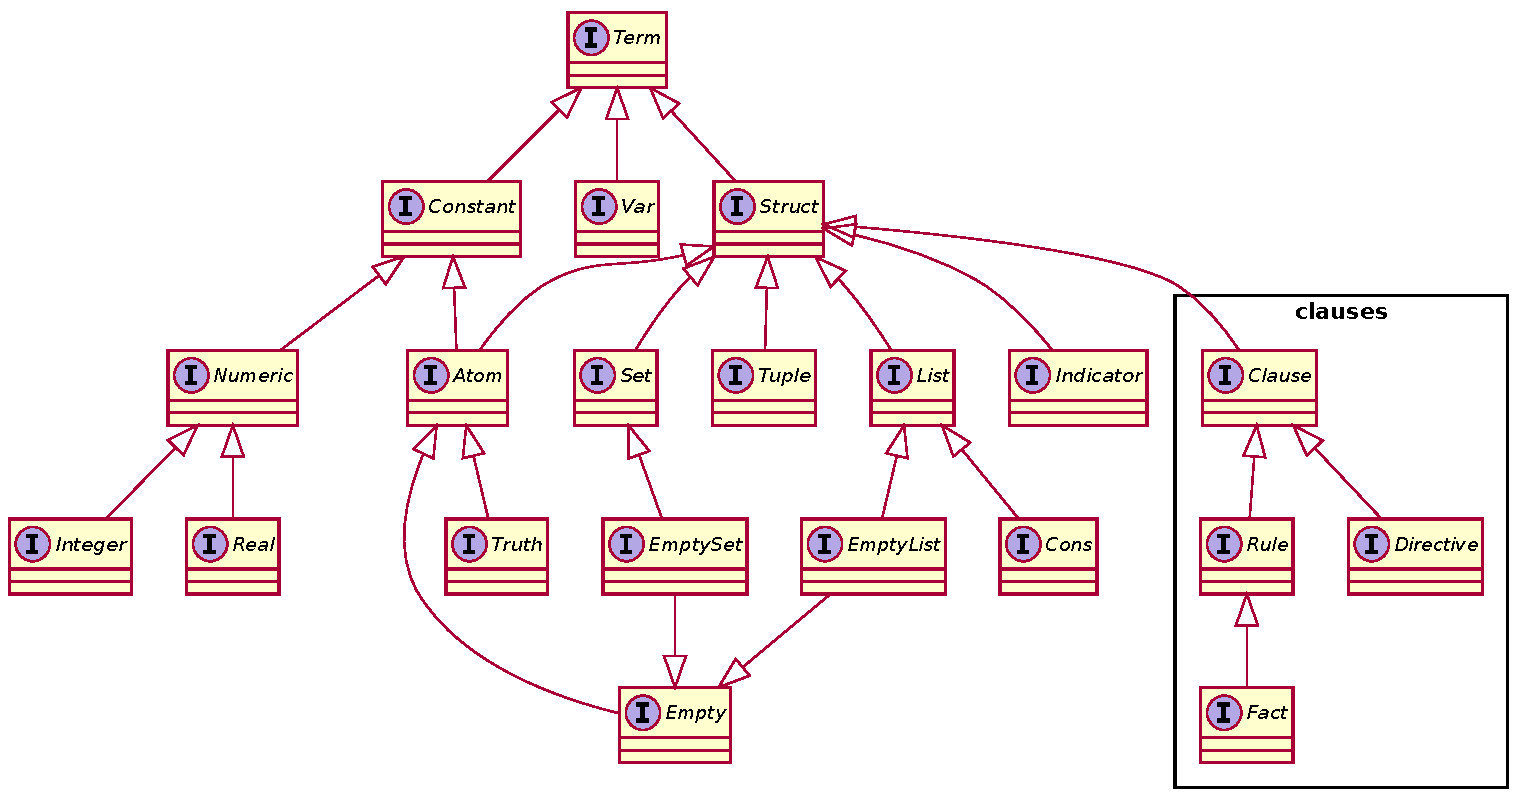
\includegraphics[width=.75\linewidth]{img/terms-nofields.pdf}
    \end{center}

    \begin{block}{Common Conventions}
        \begin{itemize}
            \item Only intefaces are publicly available, no classes
            \item Immutable design: all terms are immutable data structures
            \item The hierarchy is a DAG, not a tree
            \item Terms are totally ordered, as the are \kt{Comparable} among each others
            \item We call ``term'' any object which (indirectly) implements \kt{Term}
            %
            \begin{itemize}
                \item[!] there including clauses, i.e. instances of \kt{Clause}
            \end{itemize}
        \end{itemize}
    \end{block}
\end{frame}

\begin{frame}[allowframebreaks]{The \kt{Term} type}
    \begin{block}{The \kt{Term} type}\centering
        Base type for all terms
    \end{block}
    %
    \begin{description}
        \item[\kt{is\meta{SubType}: Boolean}] checks whether the current term is an instance of \kt{\meta{SubType}} or not
        \item[\kt{as\meta{SubType}(): \meta{SubType}}] casts the current term to \kt{\meta{SubType}} or returns null if not possible
        \item[\kt{castTo\meta{SubType}(): \meta{SubType}}] casts the current term to \kt{\meta{SubType}} or throws an exception if not possible
        \item[\kt{freshCopy(): Term}] returns a deep copy of the current term where all \kt{Var}iables have been refreshed
        \item[\kt{apply(Substitution): Term}] applies the provided \kt{Substitution} to the current \kt{Term} or throws a \kt{SubstitutionApplicationException} in case a failed \kt{Substitution} has been provided
        \item[\kt{equals(Term, Boolean): Boolean}] checks whether the provided \kt{Term} is deeply equal to the current one, letting the caller choose whether to compare variables by simple or by complete name
        \item[\kt{equals(Any?): Boolean}] checks whether the provides object is a \kt{Term} is deeply equal to the current one, comparing variables by complete names
        \item[\kt{structurallyEquals(Term): Boolean}] checks whether the provided \kt{Term} is deeply equal to the current one, in such a way that all variables are considered equal
        \item[\kt{accept<T>(TermVisitor<T>): T}] returns the object produced by letting the provided \kt{TermVisitor} visit the current \kt{Term}
        \item[\kt{compareTo(Term): Int}] compares the current \kt{Term} with the provided one, according to the total ordering on \kt{Term}s
        \item[\kt{toString(): String}] returns a representation of the current \kt{Term} for debugging purposes
        \item[\kt{variables: Sequence<Var>}] returns the (possibly empty) sequence of variables contained in the current \kt{Term}
        %
        \begin{itemize}\small
            \item[!] duplicates are \emph{not} removed
        \end{itemize}
        \item[\kt{isGround: Boolean}] returns \kt{true} if the current \kt{Term} contains no \kt{Var}iable
    \end{description}

    \framebreak

    \ktSnippet{snippets/TermUsage.kt}
\end{frame}

\begin{frame}[allowframebreaks]{Main Sorts of \kt{Term}s}
    \begin{block}{The \kt{Constant} type is a sub-type of \kt{Term}}\centering
        Base type for all constant terms (namely, strings and numbers)
    \end{block}
    %
    \begin{description}
        \item[\kt{value: Any}] returns the value of this \kt{Constant}
    \end{description}

    \begin{alertblock}{About \kt{Constant}s}
        \begin{itemize}
            \item \kt{Constant}s are inherently \alert{ground}
            \item Their \kt{isGround} property always return \kt{true}
            \item Their \kt{variables} property always return an empty sequence
        \end{itemize}
    \end{alertblock}

    \framebreak

    \begin{block}{The \kt{Numeric} type is a sub-type of \kt{Constant}}\centering
        Base type for all numeric terms (namely, reals and integers)
    \end{block}
    %
    \begin{description}
        \item[\kt{intValue: BigInteger}] returns the integer value of the current number
        %
        \begin{itemize}
            \item \kt{BigInteger}s can then be converted into \kt{Int}, \kt{Short}, etc.
            \item unlimited amount of digits $\rightarrow$ no overflow, no max value
        \end{itemize}

        \item[\kt{decimalValue: BigDecimal}] returns the decimal value of the current number
        %
        \begin{itemize}
            \item \kt{BigDecimal}s can then be converted into \kt{Double} or \kt{Float}
            \item i.e. a real number with arbitrary precision
        \end{itemize}
    \end{description}

    \framebreak

    \begin{block}{The \kt{Integer} type is a sub-type of \kt{Numeric}}\centering
        Type for all terms representing an integer number
    \end{block}
    %
    \begin{description}
        \item[\kt{value: BigInteger}] returns \kt{this.intValue}
        %
        \begin{itemize}
            \item \kt{BigInteger}s can then be converted into \kt{Int}, \kt{Short}, etc.
            \item unlimited amount of digits $\rightarrow$ no overflow, no max value
        \end{itemize}
    \end{description}

    \ktSnippet{snippets/IntUsage.kt}

    \framebreak

    \begin{block}{The \kt{Real} type is a sub-type of \kt{Numeric}}\centering
        Type for all terms representing a real number
    \end{block}
    %
    \begin{description}
        \item[\kt{value: BigDecimal}] returns \kt{this.decimalValue}
        %
        \begin{itemize}
            \item \kt{BigDecimal}s can then be converted into \kt{Double} or \kt{Float}
            \item i.e. a real number with arbitrary precision
        \end{itemize}
    \end{description}

    \ktSnippet{snippets/RealUsage.kt}

    \framebreak

    \begin{block}{The \kt{Struct} type is a sub-type of \kt{Term}}\centering
        Type for all terms of the form \kt{$f$($t_1$, \ldots, $t_N$)}, i.e. composed by a \alert{funtor} string $f$ and $N$ terms $t_1, \ldots, t_N$ called \alert{arguments}, where $N \geq 0$ is called \alert{arity}
    \end{block}
    %
    \begin{description}
        \item[\kt{functor: String}] returns $f$
        \item[\kt{arity: Int}] returns $N$
        \item[\kt{args: Array<Term>}] returns an array containing $t_1, \ldots, t_N$
        \item[\kt{argsList: List<Term>}] returns a list containing $t_1, \ldots, t_N$
        \item[\kt{argsSequence: Sequence<Term>}] returns a sequence containing $t_1, \ldots, t_N$

        \item[\kt{isFunctorWellFormed: Boolean}] returns true if the following condition hold for $f$
        %
        \begin{enumerate}\small
            \item it begins with a lower case letter
            \item it only contains letters (either lower or upper case), digits, or underscores
        \end{enumerate}
        \item[\kt{toString(): String}] returns $f$ iff $N = 0$, otherwise a string of the form
        %
        \begin{center}
            \kt{$f$($t_1$.toString(), \ldots, $t_N$.toString())}
        \end{center}
        %
        \begin{itemize}\small
            \item in both cases, $f$ is wrapped within single quotes iff \kt{isFunctorWellFormed} is false
        \end{itemize}
        \item[\kt{equals(Any?): Boolean}] compares this \kt{Struct}ure with the provided object, returning true if the latter is a \kt{Struct}ure having the same functor, arity, and arguments (which are recursively compared via \kt{equals(Any?)})
        \item[\kt{hashCode(): Int}] computes an hash code value for this \kt{Struct}ure which is coherent w.r.t. \kt{equals(Any?)}
        \item[\kt{equals(Term,Boolean): Boolean}] compares this \kt{Struct}ure with the provided object, returning true if the latter is a \kt{Struct}ure having the same functor, arity, and arguments (which are recursively compared via \kt{equals(Term,Boolean)})
        \item[\kt{structurallyEquals(Term): Boolean}] compares this \kt{Struct}ure with the provided object, returning true if the latter is a \kt{Struct}ure having the same functor, arity, and arguments (which are recursively compared via \kt{structurallyEquals(Term)})
        \item[\kt{indicator: Indicator}] returns the indicator corresponding to the current \kt{Struct}
        %
        \begin{itemize}\small
            \item i.e. the \kt{Struct}ure of the form \pl{'/'($f$, $N$)}
        \end{itemize}
        \item[\kt{get(Int): Term}] returns an argument of the current \kt{Struct} given its index
        \item[\kt{getArgAt(Int): Term}] an alias for \kt{get(Int)}
        \item[\kt{addFirst(Term): Term}] returns a novel \kt{Struct} of the form \pl{$f$($t^*$, $t_1$, \ldots, $t_N$)}, where $t^*$ is the \kt{Term} provided as argument
        \item[\kt{addLast(Term): Term}] returns a novel \kt{Struct} of the form \pl{$f$($t_1$, \ldots, $t_N$, $t^*$)}, where $t^*$ is the \kt{Term} provided as argument
        \item[\kt{append(Term): Term}] an alias for \kt{addLast(Term)}
        \item[\kt{insertAt(Int,Term): Term}] returns a novel \kt{Struct} of the form \pl{$f$($t_1$, \ldots, $t_{i-1}$, $t^*$, $t_{i+1}$, \ldots, $t_N$)}, where $t^*$ is the \kt{Term} provided as argument
        \item[\kt{setFunctor(String): Term}] returns a novel \kt{Struct} of the form \pl{$f^*$($t_1$, \ldots, $t_N$)}, where $f^*$ is the functor \kt{String} provided as argument
    \end{description}

    \framebreak

    \ktSnippet[\tiny]{snippets/StructUsage.kt}

    \framebreak

    \begin{block}{The \kt{Atom} type is a sub-type of both \kt{Struct} and \kt{Constant}}\centering
        Type for all constant 0-ary structures (i.e., with no arguments), representing strings
    \end{block}
    %
    \begin{description}
        \item[\kt{value: String}] returns \kt{this.functor}
        \item[\kt{arity: Int}] must return 0
        \item[\kt{args: Array<Term>}] must return the empty array
        \item[\kt{argsList: List<Term>}] must return the empty list
        \item[\kt{argsSequence: Sequence<Term>}] must return the empty sequence
    \end{description}

    \framebreak

    \ktSnippet{snippets/AtomUsage.kt}

    \framebreak

    \begin{block}{The \kt{Var} type is a sub-type of \kt{Term}}\centering
        Type for all variable terms, representing \alert{named} placeholders for other terms.
    \end{block}
    %
    \begin{alertblock}{About \kt{Var}iable names}
        \begin{itemize}
            \item Variables are identified by \alert{comple name}
            \item Variables' complete names are \kt{String}s of the form
            %
            \begin{center}
                \pl{$Name$\_$Identifier$}
            \end{center}
            where
            %
            \begin{description}
                \item[$Name$] is the variable's \alert{simple} name
                \item[$Identifier$] is the variable's \alert{identifier}, i.e. an im\-ple\-men\-ta\-tion-spe\-ci\-fic string aimed at distinguising \kt{Var}iables having the same simple name
            \end{description}
            \item Variables whose simple name is \pl{'\_'} are called \alert{anonymous}
        \end{itemize}
    \end{alertblock}
    %
    \begin{description}
        \item[\kt{name: String}] returns $Name$
        \item[\kt{completeName: String}] returns \pl{$Name$\_$Identifier$}
        \item[\kt{id: String}] returns $Identifier$
        \item[\kt{isAnonymous: Boolean}] returns true iff \pl{$Name$ = '\_'}
        \item[\kt{toString(): Boolean}] returns this \kt{this.completeName}
        \item[\kt{equals(Any?): Boolean}] compares this \kt{Var}iable with the provided object, returning true if the latter is a \kt{Var}iable having the same complete name
        \item[\kt{equals(Term,Boolean): Boolean}] compares this \kt{Var}iable with the provided object, returning true if the latter is a \kt{Var}iable having the same complete (resp. simple) name, assuming that the provided \kt{Boolean} is true (resp. false)
        \item[\kt{structurallyEquals(Term): Boolean}] compares this \kt{Var}iable with the provided object, returning true if the latter is a \kt{Var}iable
    \end{description}

    \ktSnippet{snippets/VarUsage.kt}

    \framebreak

    \begin{block}{The \kt{Indicator} type is a sub-type of \kt{Struct}}
        \begin{center}
            Type for all binary structures of the form
            %
            \begin{center}
                \pl{'/'($f$, $n$)}
            \end{center}
            where $f,n$ are arbitrary terms. If $f$ is an atom and $n$ is a non-negative integer, then the indicator is considered \emph{well formed}
        \end{center}
    \end{block}
    %
    \begin{description}
        \item[\kt{nameTerm: Term}] returns $f$, shortcut for \kt{get(0)}
        \item[\kt{indicatedName: String?}] if $f$ is an atom, returns \kt{$f$.value}, otherwise \kt{null}
        \item[\kt{arityTerm: Term}] returns $n$, shortcut for \kt{get(1)}
        \item[\kt{indicatedArity: Int?}] if $n$ is a non-negative integer, returns \kt{$n$.intValue.toInt()}, otherwise \kt{null}
        \item[\kt{isWellFormed: Boolean}] returns \kt{true} if the indicator is well formed
        \item[\kt{functor: String}] must return \kt{"/"}
        \item[\kt{arity: String}] must return 2
    \end{description}

    \ktSnippet{snippets/IndicatorUsage.kt}

    \framebreak

    \begin{block}{The \kt{Truth} type is a sub-type of \kt{Atom}}
        \begin{center}
            Type for special atoms representing either tautology or contradiction.
            It has only three admissible values: \pl{true} (tautology), \pl{false}, and \pl{fail} (contradictions).
        \end{center}
    \end{block}
    %
    \begin{description}
        \item[\kt{isTrue: Boolean}] returns \kt{true} if the atom is a tautology
        \item[\kt{isFail: Boolean}] returns \kt{true} if the atom is a contradiction
    \end{description}

    \ktSnippet[\tiny]{snippets/TruthUsage.kt}
\end{frame}

\begin{frame}[allowframebreaks]{Collections}
    \begin{exampleblock}{How to fold items with structures}
        \begin{itemize}
            \item Suppose you want to collect terms $t_1, \ldots, t_N$\ldots
            \item \ldots using binary structures whose functor is $f$
            \item Two folding strategies: with or without a termination term $T$
            %
            \begin{itemize}
                \item explicit termination: \pl{$f$($t_1$, $f$($t_2$, \ldots $f$($t_N$, $T$) \ldots ))}
                \item implicit termination: \pl{$f$($t_1$, $f$($t_2$, \ldots $f$($t_{N-1}$, $t_N$) \ldots ))}
            \end{itemize}
            \item A particular collection is therefore determined by:
            %
            \begin{itemize}
                \item the particular choice of $f$
                \item the particular folding strategy adopted
                \item the particular termination term $T$, if any
            \end{itemize}
        \end{itemize}
    \end{exampleblock}
    %
    \begin{block}{The \kt{Collection} type is a sub-type of \kt{Struct}}\centering
        Base type for all right-recursive structures aimed at containing an unlimited amount of terms.
    \end{block}
    %
    \begin{description}
        \item[\kt{unfoldedSequence: Sequence<Term>}] in general, returns a sequence containing the terms $t_1, \ldots, t_N$, plus $T$ in case of explicit folding strategy
        \item[\kt{unfoldedList: List<Term>}] in general, returns a list containing the terms $t_1, \ldots, t_N$, plus $T$ in case of explicit folding strategy
        \item[\kt{unfoldedArray: Array<Term>}] in general, returns an array containing the terms $t_1, \ldots, t_N$, plus $T$ in case of explicit folding strategy
        \item[\kt{size: Int}] in general, returns $N$
        \item[\kt{toSequence(): Sequence<Term>}] in general, returns a sequence containing the terms $t_1, \ldots, t_N$
        \item[\kt{toList(): List<Term>}] in general, returns a list containing the terms $t_1, \ldots, t_N$
        \item[\kt{toArray(): Array<Term>}] in general, returns an array containing the terms $t_1, \ldots, t_N$
        \item[\kt{unfold(): Sequence<Term>}] in general, returns a sequence containing the terms \pl{$f$($t1$, $f$($t_2$, \ldots))}, \pl{$f$($t_2$, \ldots)}, \pl{\ldots}, plus $T$ in case of explicit folding strategy, or \pl{$f$($t_{N-1}$, $t_N$)} otherwise
    \end{description}

    \framebreak

    \begin{block}{The \kt{List} type is a sub-type of \kt{Collection}}
        \begin{center}
            Base type for logic lists, i.e. collections using \pl{'.'} as functor and \pl{'[]'} as the termination term.
            %
            So all lists are terms of the form
            \begin{center}
                \pl{'.'($t_1$, '.'($t_2$, \ldots '.'($t_N$, $T$)\ldots))}.
            \end{center}
            %
            A list is considered well formed iff $T \equiv \pl{[]}$.
        \end{center}
    \end{block}
    %
    \begin{alertblock}{About logic lists}
        \begin{itemize}
            \item There are two sub-types of \kt{List}:
            %
            \begin{itemize}
                \item \alert{\kt{Cons}}, capturing all terms of the form \pl{'.'($h$, $t$)} where both $h$ and $t$ are terms of any sort
                \item \alert{\kt{EmptyList}}, which has only one value, namely the atom \pl{'[]'}
            \end{itemize}

            \item Logic lists are represented as strings using the following notation:
            %
            \begin{center}
                \pl{[$t_1$, $t_2$, \ldots $t_n$ | $T$]}
            \end{center}
            %
            \begin{itemize}
                \item where `\pl{| $T$}' may be omitted in case $T \equiv \pl{[]}$
            \end{itemize}
        \end{itemize}
    \end{alertblock}
    %
    \begin{description}
        \item[\kt{isWellFormed: Boolean}] returns \kt{true} if the list is well formed
        \item[\kt{last: Term}] returns $T$
        \item[\kt{isCons: Boolean}] returns \kt{true} if the list is not empty
        \item[\kt{isEmptyList: Boolean}] returns \kt{true} if the list is empty
        \item[\kt{unfoldedSequence: Sequence<Term>}] returns a sequence containing the terms $t_1, \ldots, t_N, \pl{[]}$
        \item[\kt{unfoldedList: List<Term>}] returns a list containing the terms $t_1, \ldots, t_N, \pl{[]}$
        \item[\kt{unfoldedArray: Array<Term>}] returns an array containing the terms $t_1, \ldots, t_N, \pl{[]}$
        \item[\kt{size: Int}] returns $N$ if the list is well formed, or $N+1$ otherwise
        \item[\kt{toSequence(): Sequence<Term>}] returns a sequence containing the terms $t_1, \ldots, t_N$, plus $T$ iff $T \not\equiv \pl{[]}$
        \item[\kt{toList(): List<Term>}] returns a list containing the terms $t_1, \ldots, t_N$, plus $T$ iff $T \not\equiv \pl{[]}$
        \item[\kt{toArray(): Array<Term>}] returns an array containing the terms $t_1, \ldots, t_N$, plus $T$ iff $T \not\equiv \pl{[]}$
        \item[\kt{unfold(): Sequence<Term>}] returns a sequence containing the terms \pl{'.'($t1$, '.'($t_2$, \ldots))}, \pl{'.'($t_2$, \ldots)}, \pl{\ldots}, $T$
    \end{description}

    \ktSnippet[\tiny]{snippets/ListUsage.kt}

    \framebreak

    \begin{block}{The \kt{Tuple} type is a sub-type of \kt{Collection}}
        \begin{center}
            Base type for logic conjunctions, i.e. collections using \pl{','} as functor and an implicit termination strategy.
            %
            So all tuples are terms of the form
            \begin{center}
                \pl{','($t_1$, ','($t_2$, \ldots ','($t_{N-1}$, $t_N$)\ldots))}.
            \end{center}
            %
            Notice that tuples always contain at least 2 terms.
        \end{center}
    \end{block}
    %
    \begin{alertblock}{About logic tuples}
        \begin{itemize}
            \item Logic tuples are represented as strings using the following notation:
            %
            \begin{center}
                \pl{($t_1$, $t_2$, \ldots $t_n$)}
            \end{center}
        \end{itemize}
    \end{alertblock}
    %
    \begin{description}
        \item[\kt{unfoldedSequence: Sequence<Term>}] returns a sequence containing the terms $t_1, \ldots, t_N$
        \item[\kt{unfoldedList: List<Term>}] returns a list containing the terms $t_1, \ldots, t_N$
        \item[\kt{unfoldedArray: Array<Term>}] returns an array containing the terms $t_1, \ldots, t_N$
        \item[\kt{size: Int}] returns $N$
        \item[\kt{toSequence(): Sequence<Term>}] returns \kt{this.unfoldedSequence}
        \item[\kt{toList(): List<Term>}] returns \kt{this.unfoldedList}
        \item[\kt{toArray(): Array<Term>}] returns \kt{this.unfoldedArray}
        \item[\kt{unfold(): Sequence<Term>}] returns a sequence containing the terms \pl{','($t1$, ','($t_2$, \ldots))}, \pl{','($t_2$, \ldots)}, \pl{\ldots}, \pl{','($t_{N-1}$, $t_N$)}
    \end{description}

    \ktSnippet{snippets/TupleUsage.kt}

    \framebreak

    \begin{block}{The \kt{Set} type is a sub-type of \kt{Collection}}
        \begin{center}
            Base type for logic sets, i.e. a particular sort of collection using \pl{\{\}} as functor, which may either be empty or contain a single term---which may possibly be a tuple.
        \end{center}
    \end{block}
    %
    \begin{alertblock}{About logic sets}
        \begin{itemize}
            \item There are two sub-types of \kt{Set}:
            %
            \begin{itemize}
                \item \alert{\kt{Set}}, capturing all terms of the form \pl{'\{\}'($x$)} where $x$ is a term of any sort
                \item \alert{\kt{EmptySet}}, which has only one value, namely the atom \pl{'\{\}'}
            \end{itemize}

            \item Logic sets are represented as strings using the following notations:
            %
            \begin{itemize}
                \item \pl{\{\}} in case of empty set
                \item \pl{\{$t_1$, \ldots $t_N$\}} in case $x$ $\equiv$ \pl{($t_1$, \ldots, $t_N$)}, i.e. if $x$ is a tuple
                \item \pl{\{$x$\}} otherwise
            \end{itemize}
        \end{itemize}
    \end{alertblock}
    %
    \begin{description}
        \item[\kt{unfoldedSequence: Sequence<Term>}] returns a sequence containing the terms $t_1, \ldots, t_N$ if $x$ is a tuple, just $x$ otherwise, or nothing if the set is empty
        \item[\kt{unfoldedList: List<Term>}] returns a list containing the terms $t_1, \ldots, t_N$ if $x$ is a tuple, just $x$ otherwise, or nothing if the set is empty
        \item[\kt{unfoldedArray: Array<Term>}] returns an array containing the terms $t_1, \ldots, t_N$ if $x$ is a tuple, just $x$ otherwise, or nothing if the set is empty
        \item[\kt{size: Int}] returns $N$ if $x$ is a tuple, 1 otherwise, or 0 if the set is empty
        \item[\kt{toSequence(): Sequence<Term>}] returns \kt{this.unfoldedSequence}
        \item[\kt{toList(): List<Term>}] returns \kt{this.unfoldedList}
        \item[\kt{toArray(): Array<Term>}] returns \kt{this.unfoldedArray}
    \end{description}

    \ktSnippet{snippets/SetUsage.kt}

\end{frame}

\begin{frame}[allowframebreaks]{Clauses}
    \begin{block}{The \kt{Clause} type is a sub-type of \kt{Struct}}\centering
        Base type for all structures aimed at representing Horn clauses.
        They all use \pl{':-'} as functor and carry either 1 or 2 arguments, named \emph{head} and \emph{body}.
    \end{block}
    %
    \begin{alertblock}{About clauses}
        \begin{itemize}
            \item There are three sub-types of \kt{Clause}:
            %
            \begin{itemize}
                \item \alert{\kt{Rule}}, capturing all structures of the form \pl{':-'($h$, $b$)} where $h$ is a \kt{Struct}ure and $b$ is a term of any sort
                %
                \begin{itemize}
                    \item \alert{\kt{Fact}}, capturing all rules of the form \pl{':-'($h$, true)}, where $b$ $\equiv$ \pl{true}
                \end{itemize}
                \item \alert{\kt{Directives}}, capturing all structures of the form \pl{':-'($b$)} where $b$ is a term of any sort
            \end{itemize}

            \item Logic clauses are represented as strings using the following notations:
            %
            \begin{itemize}
                \item \pl{$h$ :- $b_1$, \ldots, $b_N$.} in case of rules where $b$ $\equiv$ \pl{($b_1$, \ldots, $b_N$)}
                \item \pl{$h$ :- $b$.} in case of rules
                \item \pl{$h$.} in case of facts
                \item \pl{:- $b_1$, \ldots, $b_N$.} in case of directives where $b$ $\equiv$ \pl{($b_1$, \ldots, $b_N$)}
                \item \pl{:- $b$.} in case of directives
            \end{itemize}
        \end{itemize}
    \end{alertblock}
    %
    \framebreak
    %
    \begin{description}
        \item[\kt{head: Struct?}] returns $h$ for rules, or \kt{null} for directives
        \item[\kt{body: Term}] returns $b$
        \item[\kt{isRule: Boolean}] returns \kt{true} if the clause is not a directive
        \item[\kt{isDirective: Boolean}] returns \kt{true} if the clause is a directive
        \item[\kt{isFact: Boolean}] returns \kt{true} if the clause is a fact
        \item[\kt{isWellFormed: Boolean}] returns \kt{true} iff no sub-term in $b$ which is interpretable as a logic goal is a \kt{Var}iable
    \end{description}

    \framebreak

    \ktSnippet[\tiny]{snippets/ClausesUsage.kt}
\end{frame}

\subsubsection{Creating \kt{Term}s}

\begin{frame}[allowframebreaks]{Creating \kt{Term}s via Static Factories}

    Conventions on terms/clause creation in \twopkt:
    %
    \bigskip
    %
    \begin{itemize}
        \item Terms and clauses can be created via \alert{static factory methods} on interfaces
        %
        \ktSnippet{./snippets/TermsCreation.kt}

        \framebreak

        \item Factory methods always instantiate the most specific type possible:
        %
        \ktSnippet{./snippets/SpecificTermsCreation.kt}
    \end{itemize}

    \framebreak

    \begin{block}{Creating \kt{Integer}s}
        \begin{description}
            \item[\kt{Integer.of(\meta{Kotlin Integer Type})}] creates an \kt{Integer} out of a Kotlin integer
            \item[\kt{Integer.of(BigInteger)}] creates an \kt{Integer} out of a \kt{BigInteger}
            \item[\kt{Integer.of(String,Int)}] parses the string as an \kt{Integer} with the provided base
            \item[\kt{Integer.ZERO}] constant for the \kt{Integer} equal to 0
            \item[\kt{Integer.ONE}] constant for the \kt{Integer} equal to 1
            \item[\kt{Integer.MINUS\_ONE}] constant for the \kt{Integer} equal to -1
        \end{description}
    \end{block}

    \framebreak

    \begin{block}{Creating \kt{Real}s}
        \begin{description}
            \item[\kt{Real.of(\meta{Kotlin Floating Type})}] creates a \kt{Real} out of a Kotlin float
            \item[\kt{Real.of(BigInteger)}] creates a \kt{Real} out of a \kt{BigDecimal}
            \item[\kt{Real.of(String)}] parses the string as a \kt{Real}
            \item[\kt{Real.ZERO}] constant for the \kt{Real} equal to 0.0
            \item[\kt{Real.ONE}] constant for the \kt{Real} equal to 1.0
            \item[\kt{Real.MINUS\_ONE}] constant for the \kt{Real} equal to -1.0
            \item[\kt{Real.ONE\_HALF}] constant for the \kt{Real} equal to 0.5
            \item[\kt{Real.ONE\_TENTH}] constant for the \kt{Real} equal to 0.1
        \end{description}
    \end{block}

    \framebreak

    \begin{block}{Creating \kt{Atom}s}
        \begin{description}
            \item[\kt{Atom.of(String)}] creates an \kt{Atom} out of a string
            %
            \begin{itemize}\small
                \item returns a \kt{Truth} if \kt{"true"}, \kt{"false"}, or \kt{"fail"} is passed
                \item returns an \kt{EmptyList} if \kt{"[]"} is passed
                \item returns an \kt{EmptySet} if \kt{"\{\}"} is passed
            \end{itemize}
        \end{description}
    \end{block}

    \framebreak

    \begin{block}{Creating \kt{Var}iables}
        \begin{description}
            \item[\kt{Var.of(String)}] creates an \kt{Var}iable out of a string
            %
            \begin{itemize}\small
                \item the string is considered as the \kt{Var}iable's \alert{simple} name
                \item[!] there is \alert{no way} to create a \kt{Var}iable with a particular \alert{complete} name
            \end{itemize}

            \item[\kt{Var.anonymous()}] creates an anonymous \kt{Var}iable
        \end{description}
    \end{block}

    \ktSnippet{snippets/VarCreation.kt}

    \framebreak

    \begin{block}{Creating \kt{Struct}ures}
        \begin{description}
            \item[\kt{Struct.of(String,\meta{Container})}] creates an \kt{Struct}ure with the given functor and arguments
            %
            \begin{itemize}\small
                \item where \kt{\meta{Container}} may be an iterable, a sequence, or a varargs of \kt{Term}s
            \end{itemize}

            \item[\kt{Struct.template(String,Int)}] creates an \kt{Struct}ure with the given functor and arity, whose arguments are all anonymous variables

            \item[\kt{Struct.fold(String,\meta{Container},Term?)}] folds the terms in \kt{\meta{Container}} using the provided functor recursively, adopting either an explicit or implicit folding strategy depending on whether the last argument is null or not
        \end{description}
    \end{block}

    \ktSnippet[\tiny]{snippets/StructCreation.kt}

\end{frame}

\begin{frame}[allowframebreaks]{Creating \kt{Collection}s via Static Factories}
    \begin{block}{Creating \kt{List}s}
        \begin{description}
            \item[\kt{List.empty()}] creates an \kt{EmptyList}

            \item[\kt{Empty.list()}] creates an \kt{EmptyList}

            \item[\kt{List.of(\meta{Container})}] creates a \kt{[]}-terminated \kt{List} containing all the terms in \kt{\meta{Container}}
            %
            \begin{itemize}\small
                \item where \kt{\meta{Container}} may be an iterable, a sequence, or a varargs of \kt{Term}s
            \end{itemize}

            \item[\kt{List.from(\meta{Container},Term?)}] creates a \kt{List} containing all the terms in \kt{\meta{Container}} and terminated by either the last argument, if it is non-null, or be the last term in \kt{\meta{Container}}, otherwise

            \item[\kt{Cons.singleton(Term)}] creates \kt{List} containing just one item

            \item[\kt{Cons.of(Term,Term)}] creates a term of the form \kt{'.'($t_1$, $t_2$)} where $t_1,t_2$ are the first and second arguments, respectively
        \end{description}
    \end{block}

    \framebreak

    \ktSnippet[\tiny]{snippets/ListCreation.kt}

    \framebreak

    \begin{block}{Creating \kt{Tuple}s}
        \begin{description}
            \item[\kt{Tuple.of(Term,Term,\meta{Container})}] creates a \kt{Tuple} containing at least 2 terms, other than the ones in \kt{\meta{Container}}
            %
            \begin{itemize}\small
                \item where \kt{\meta{Container}} may be a (possibly empty) iterable, a sequence, or a varargs of \kt{Term}s
            \end{itemize}
        \end{description}
    \end{block}

    \framebreak

    \begin{block}{Creating \kt{Set}s}
        \begin{description}
            \item[\kt{Set.empty()}] creates an \kt{EmptySet}

            \item[\kt{Empty.set()}] creates an \kt{EmptySet}

            \item[\kt{Set.of(\meta{Container})}] creates a \kt{Set} containing all the terms in \kt{\meta{Container}}
            %
            \begin{itemize}\small
                \item where \kt{\meta{Container}} may be an iterable, a sequence, or a varargs of \kt{Term}s
            \end{itemize}
        \end{description}
    \end{block}
\end{frame}

\begin{frame}[allowframebreaks]{Creating \kt{Clause}s via Static Factories}
    \begin{block}{Creating \kt{Clause}s}
        \begin{description}
            \item[\kt{Clause.of(Struct?,\meta{Container})}] creates either a \kt{Directive} or a \kt{Rule} depending on whether the provide \kt{Struct} is \kt{null} or not. In both cases items in \kt{\meta{Container}} compose the body of the clause, whereas the \kt{Struct} is an optional head
            %
            \begin{itemize}\small
                \item where \kt{\meta{Container}} may be an iterable, a sequence, or a varargs of \kt{Term}s
                \item[!] in any case, if \kt{\meta{Container}} contains at least 2 terms, a \kt{Tuple} is created behind the scenes
            \end{itemize}

            \item[\kt{Rule.of(Struct,\meta{Container})}] creates a \kt{Rule} using provided \kt{Struct} as head and the \emph{conjunction} of terms in \kt{\meta{Container}} as body
            %
            \begin{itemize}\small
                \item[!] returns a \kt{Fact} is \kt{\meta{Container}} is empty
            \end{itemize}

            \item[\kt{Fact.of(Struct)}] creates a \kt{Fact} given the \kt{Struct} acting as head
        \end{description}
    \end{block}
\end{frame}

\subsubsection{About \kt{Term}s' Design}

\begin{frame}[allowframebreaks]{Identity vs. Equalities}
    \begin{block}{Terms Identity}
        Two terms are \alert{identical} iff:
        %
        \begin{itemize}
            \item both are \kt{Integer}s having the same value
            \item both are \kt{Real}s having the same value
            \item both are \kt{Atom}s having the same value
            \item both are \kt{Var}iables having the same \alert{complete} name
            \item both are \kt{Struct}ures having the same
            %
            \begin{itemize}
                \item functor, and arity
                \item their arguments are pair-wise \alert{identical}
            \end{itemize}
        \end{itemize}
    \end{block}
    %
    \begin{itemize}
        \item Terms' \alert{identity} is tested via \kt{Term.equals(Any?)}
        \item or via \kt{Term.equals(Term, \alert{true})}
        \item or via \kt{$t_1$ == $t_2$} (because of \alert{Kotlin's operator overloading})
        %
        \begin{itemize}
            \item in Kotlin, objects' identity is tested via \kt{$t_1$ === $t_2$})
        \end{itemize}
    \end{itemize}

    \framebreak

    \begin{block}{Terms Equality}
        Two terms are \alert{equal} iff:
        %
        \begin{itemize}
            \item both are \kt{Integer}s having the same value
            \item both are \kt{Real}s having the same value
            \item both are \kt{Atom}s having the same value
            \item both are \kt{Var}iables having the same \alert{simple} name
            \item both are \kt{Struct}ures having the same
            %
            \begin{itemize}
                \item functor, and arity
                \item their arguments are pair-wise \alert{equal}
            \end{itemize}
        \end{itemize}
    \end{block}
    %
    \begin{itemize}
        \item Terms' \alert{equality} is tested via \kt{Term.equals(Term, \alert{false})}
    \end{itemize}

    \framebreak

    \begin{block}{Terms Structural Equality}
        Two terms are \alert{structurally equal} iff:
        %
        \begin{itemize}
            \item both are \kt{Numbers}s having the same value
            \item both are \kt{Atom}s having the same value
            \item both are \kt{Var}iables
            \item both are \kt{Struct}ures having the same
            %
            \begin{itemize}
                \item functor, and arity
                \item their arguments are pair-wise \alert{structurally equal}
            \end{itemize}
        \end{itemize}
    \end{block}
    %
    \begin{itemize}
        \item Terms' \alert{structural equality} is tested via \kt{Term.structurallyEquals(Term)}
    \end{itemize}

    \framebreak

    \ktSnippet{snippets/TermEqualities.kt}
\end{frame}

\begin{frame}[allowframebreaks]{Total Ordering of Terms}
    \begin{block}{Overview}
        \begin{itemize}
            \item Terms are totally ordered
            \item Terms are comparable according to the default ordering
            \item Interface \kt{TermComparator} aims to compare terms according to some custom ordering
            \item \kt{TermComparator.DefaultComparator} implements the default ordering of terms
            \item \kt{Term.compareTo} exploits \kt{DefaultComparator} by default
        \end{itemize}
    \end{block}

    \begin{exampleblock}{Default ordering of terms}
        \[ \kt{Var} < \kt{Real} < \kt{Integer} < \kt{Atom} < \kt{Struct} \]
        %
        \begin{itemize}
            \item variables are lexicographically ordered by complete name
            \item numbers are ascendantly ordered by value
            \item atoms are lexicographically ordered by value
            \item structures are ordered by
            %
            \begin{enumerate}
                \item by arity, ascendantly
                \item then by functor, lexicographically
                \item then by $1^{st}$ argument
                \item then by $2^{nd}$ argument
                \item[\vdots]
            \end{enumerate}
        \end{itemize}
    \end{exampleblock}

    \framebreak

    \ktSnippet{snippets/TermOrdering.kt}
\end{frame}

\begin{frame}[allowframebreaks]{Terms' Immutability}

    \begin{alertblock}{Takeaway}\centering
        All terms are \alert{immutable}
    \end{alertblock}

    \begin{block}{Consequences}
        \begin{itemize}
            \item Terms cannot be modified
            %
            \begin{itemize}
                \item[$\rightarrow$] terms are \alert{side-effect free}
                \item[$\rightarrow$] caching \& instance re-use can be exploited pervasively
                \item[$\rightarrow$] no concurrency issue
            \end{itemize}
            \item They must always be re-created from scratch, upon edit
            \item Editing a term implies creating a copy of that term
            \item Thus, many operations imply term copying:
            %
            \begin{itemize}
                \item assigning a value to a variable
                \item applying a substitution to a term
                \item altering some structure's arguments/functor
                \item refreshing some term's variables
                \item[\ldots]
            \end{itemize}

            \smallskip

            \item[!] Cloning a \alert{deep} term may be time consuming
        \end{itemize}
    \end{block}

    \begin{exampleblock}{About Cloning Lists}
        \begin{itemize}
            \item Lists are very likely to become very deep
            \item[$\rightarrow$] List cloning is made lazy to save computational resources
        \end{itemize}
    \end{exampleblock}
\end{frame}

\subsection{\kt{Var}iables and \kt{Scope}s}

\begin{frame}[allowframebreaks]{Conventions for \kt{Var}iables}
    \begin{block}{About Variables Creation}
        \begin{itemize}
            \item Variables are always created \alert{different}
            \item There is no way to create two equals variables
            %
            \begin{itemize}
                \item[!] this is deliberate
            \end{itemize}
        \end{itemize}
    \end{block}

    \begin{itemize}
        \item[$\rightarrow$] To create a term where the same variable occurs more than once\ldots
        %
        \begin{itemize}
            \item \ldots a reference to the variable should be locally saved somehow
        \end{itemize}
    \end{itemize}

    \framebreak

    \ktSnippet[\tiny]{snippets/VarReuse.kt}

\end{frame}

\begin{frame}[allowframebreaks]{The need for \kt{Scope}s}
    \begin{block}{\kt{Scope}s}\centering
        Scopes are \alert{factories} of terms allowing re-use of variables
    \end{block}

    \begin{alertblock}{Why \kt{Scope}s}
        \begin{itemize}
            \item Instances of \kt{Scope} expose methods to create \kt{Terms}
            \item Alternative to create \kt{Term}s via \alert{static factories}
            \item Instances of variables are cached \alert{by simple name}
            \item[$\rightarrow$] Purpose: reusing \kt{Var}iables while creating \kt{Term}s
        \end{itemize}
    \end{alertblock}

    \begin{description}
        \item[\kt{variables: Map<String, Var>}] returns all the \kt{Var}iables created so far in this \kt{Scope}, indexed by \emph{simple} name
        \item[\kt{varOf(String}: Var] returns a \kt{Var} having the provided simple, name possibly re-using some entry of \kt{variables}, if possible, or creating a new one, otherwise
        \item[\kt{anonymous(): Var}] alias for \kt{Var.anonymous}
        \item[\kt{atomOf(String): Atom}] alias for \kt{Atom.of}
        \item[\kt{structOf(String, \meta{Container}): Struct}] alias for \kt{Struct.of}
        %
        \begin{itemize}\small
            \item where \kt{\meta{Container}} may be an iterable, a sequence, or a varargs of \kt{Term}s
        \end{itemize}
        \item[\vdots]
    \end{description}
    %
    \begin{itemize}
        \item (one method exists in \kt{Scope} for each static factory described before)
    \end{itemize}

    \begin{block}{How to create \kt{Scope}s}
        \begin{description}
            \item[\kt{Scope.empty()}] creates a new empty \kt{Scope}

            \item[\kt{Scope.empty(Scope.()->R): R}] creates a new empty \kt{Scope} and accepts a lambda with receiver aimed at creating an object of type \kt{R} using that \kt{Scope}
            %
            \begin{itemize}
                \item can be used via the syntax \kt{Scope.empty \{ \meta{Code} \}} in Kotlin
            \end{itemize}
        \end{description}
    \end{block}

    \framebreak

    \ktSnippet{snippets/ScopeUsage.kt}
\end{frame}

\subsection{\kt{Subtitution}s as First Class Entities}

\begin{frame}[allowframebreaks]{The \kt{Substitution} Type Hierarchy}
    \begin{center}
        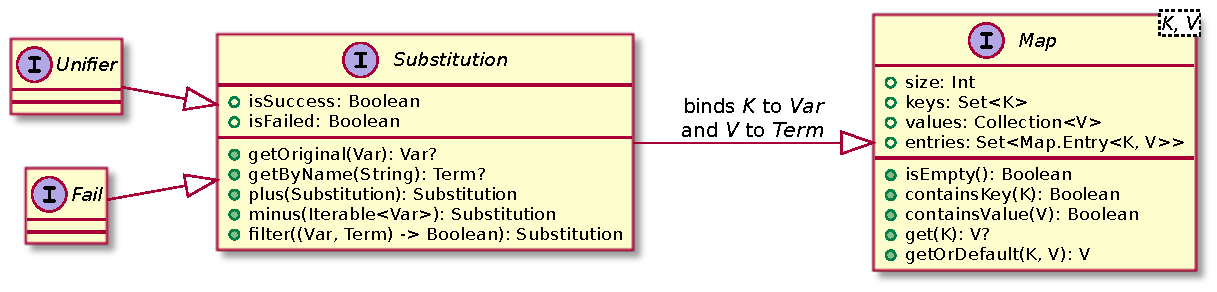
\includegraphics[width=.8\linewidth]{img/substitutions.pdf}
    \end{center}

    \begin{block}{The \kt{Substitution} type}\centering
        \begin{center}
            Base type for all \alert{substitutions} i.e. assignments of \kt{Var}iables to \kt{Term}s
        \end{center}
        %
        \begin{itemize}
            \item \kt{Substitution} is a sub-type of \kt{Map<Var, Term>}

            \item There are two sub-types of \kt{Substitution}:
            %
            \begin{itemize}
                \item \alert{\kt{Unifier}s}, actually mapping a (possibly empty) set of \kt{Var}s to their corresponding \kt{Term}
                %
                \begin{itemize}
                    \item[ie] an object of the form \kt{\{$v_1$=$t_1$, \ldots, $v_n$=$t_n$\}} where $t \geq 0$, all $v_i$ are \kt{Var}iables, and all $t_i$ are \kt{Term}s
                    \item[!] the empty mapping is an admissible unifier
                \end{itemize}
                \item \alert{\kt{Fail}}, representing the \alert{failed} substitution
            \end{itemize}

            \item Both \kt{Unifier} and \kt{Fail} are nested types of \kt{Substitution}
        \end{itemize}
    \end{block}

    \begin{description}
        \item[\kt{isSuccess: Boolean}] checks whether the current \kt{Substitution} is a \kt{Unifier}
        \item[\kt{isFail: Boolean}] checks whether the current \kt{Substitution} is \kt{Fail}ed
        \item[\kt{getByName(String): Term?}] gets the value of a \kt{Var}iable by its \emph{simple} name
        \item[\kt{plus(Substitution): Substitution}] merges the current \kt{Substitution} with the provided one (a third one is created)
        \item[\kt{minus(\meta{Container}): Substitution}] returns a knew \kt{Substitution} \alert{not} containing any \kt{Var} contained in \kt{\meta{Container}}
        %
        \begin{itemize}\small
            \item where \kt{\meta{Container}} is an iterable, sequence, or vararg of \kt{Var}iables
        \end{itemize}
        \item[\kt{minus(Substitution): Substitution}]  returns a knew \kt{Substitution} \alert{not} containing any \kt{Var} contained in the provided \kt{Substitution}
        \item[\kt{filter(\meta{Container}): Substitution}] returns a knew \kt{Substitution} containing \alert{only} the \kt{Var}iables contained in the provided \kt{\meta{Container}}
        \item[\kt{filter(\meta{Predicate}): Substitution}] returns a knew \kt{Substitution} containing \alert{only} the \kt{Var}iables contained for which \kt{\meta{Predicate}} is \kt{true}
    \end{description}
    %
    \begin{itemize}
        \item[+] methods \& properties of \kt{Map} such as \kt{get}, \kt{size}, etc.
    \end{itemize}

    \framebreak

    \begin{alertblock}{\kt{Substitution}s can be merged}
        Assuming that:
        %
        \begin{itemize}
            \item $U_1 = $ \kt{\{$X_1$=$t_1$, \ldots, $X_n$=$t_n$\}} is a unifier
            \item $U_2 = $ \kt{\{$Y_1$=$t'_1$, \ldots, $Y_m$=$t'_m$\}} is another unifier
            \item $\emptyset$ denotes the failed substitution
        \end{itemize}
        %
        \[U_1 + U_2 = \begin{cases}
            \text{\kt{\{$X_1$=$t_1$, \ldots, $X_n$=$t_n$, $Y_1$=$t'_1$, \ldots, $Y_m$=$t'_m$\}}} \\
            \qquad\text{ if } \nexists i,j : X_i = Y_j \\
            \text{\kt{\{$X_1$=$t_1$, \ldots, $Y_i$=$t'_j$, \ldots, $Y_m$=$t'_m$\}}} \\
            \qquad\text{ if } \forall i,j : X_i = Y_j \implies t_i = t'_j\\
            \emptyset \text{ otherwise }
        \end{cases}\]
        %
        \[ U_1 + \emptyset = \emptyset + U_2 = \emptyset \]
    \end{alertblock}

    \ktSnippet[\tiny]{snippets/SubstitutionUsage.kt}

\end{frame}

\begin{frame}{Creating \kt{Substitution}s}
    \begin{block}{Static factories for \kt{Substitution}s}
        \begin{description}
            \item[\kt{Substitution.failed()}] return an instance of \kt{Fail}
            %
            \item[\kt{Substitution.of(\meta{KeyValuePairs})}] creates a new \kt{Substition} using the provided key-value pairs, where
            %
            \begin{itemize}\small
                \item keys can be either strings or \kt{Var}s
                \item values can be arbitrary \kt{Term}s
                \item multiple pairs can be provided
                \item if the same \kt{Var} is assigned to different \kt{Term}s, an instance of \kt{Fail} is returned
            \end{itemize}

            \item[\kt{Substitution.unifier(\meta{KeyValuePairs})}] creates a new \kt{Unifier} using the provided key-value pairs, where
            %
            \begin{itemize}\small
                \item if the same \kt{Var} is assigned to different \kt{Term}s, a \alert{\kt{SubstitutionException}} is thrown
            \end{itemize}
        \end{description}
    \end{block}
\end{frame}

\begin{frame}[allowframebreaks]{Applying Substitutions to Terms}
    \begin{block}{Definition and Notation}
        Let
        \begin{itemize}
            \item $t$ be a term
            \item $U = $ \kt{\{$X_1$=$t_1$, \ldots, $X_n$=$t_n$\}} be a unifier
        \end{itemize}
        then we denote by
        \[t' = t[U]\]
        the term attained by \alert{applying} $U$ to $t$.
        %
        \begin{itemize}
            \item $t'$ has the same structure of $t$\ldots
            \item \ldots except each occurrence of $X_i$ is replaced by $t_i$
        \end{itemize}
    \end{block}

    \begin{alertblock}{Notable Cases}
        \begin{itemize}
            \item Applying the failed substitution $\emptyset$ to any term $t$ makes no sense
            \item If $x$ is \alert{ground} then $x[U] = x$, $\forall U$
        \end{itemize}
    \end{alertblock}

    \begin{block}{In practice}
        Let $t$ denote a \kt{Term} and $s$ denote a \kt{Substitution}:
        \begin{description}
            \item[\kt{$t$.apply(Substitution): Term}] returns a new \kt{Term} attained by applying the provided \kt{Substitution} to $t$
            %
            \begin{itemize}\small
                \item may throw a \alert{\kt{SubstitutionApplicationException}} if the \kt{Substitution} is an instance of \kt{Fail} at run time
            \end{itemize}

            \item[\kt{$t$.get(Substitution): Term}] is an alias for \kt{$t$.apply}
            %
            \begin{itemize}
                \item this can be invoked via the syntax \alert{\kt{$t$[$s$]}} in Kotlin
            \end{itemize}

            \item[\kt{$s$.applyTo(Term)}: Term] returns a new \kt{Term} attained by applying $s$ to the provided \kt{Term}
            %
            \begin{itemize}\small
                \item may throw a \alert{\kt{SubstitutionApplicationException}} if the $s$ is an instance of \kt{Fail} at run time
            \end{itemize}
        \end{description}
    \end{block}

    \ktSnippet[\tiny]{snippets/SubstitutionApplication.kt}
\end{frame}

\begin{frame}[allowframebreaks]{Refreshing Terms}
    \begin{block}{Definition and Notation}
        Let $t$ be a \kt{Term} and suppose that $t$:
        %
        \begin{itemize}
            \item is \alert{compound} (i.e. it is a \kt{Struct})
            \item it contains some \kt{Var}iables $X_1$, \ldots, $X_n$
        \end{itemize}
        %
        then \alert{refreshing} $t$ means creating another term $t'$ such that:
        %
        \begin{itemize}
            \item $t'$ has the same structure of $t$
            \item each occurrence of $X_i$ is replaced by $X'_i$, where
            %
            \begin{itemize}
                \item $X'_i$ is a fresh variable s.t. $X'_i \neq X_i$
                \item $X'_i$ has the same name of $X_i$
            \end{itemize}
        \end{itemize}
    \end{block}

    \begin{alertblock}{Notable Cases}
        \begin{itemize}
            \item If $t$ is \alert{ground} then refreshing $t$ leaves it unaffected
        \end{itemize}
    \end{alertblock}

    \begin{block}{In practice}
        Let $t$ denote a \kt{Term}:
        %
        \begin{description}
            \item[\kt{$t$.freshCopy(): Term}] returns a new \kt{Term} attained by refreshing $t$
            %
            \begin{itemize}\small
                \item the new \kt{Term} is guaranteed to only contain \kt{Var}iables which have \alert{never} been used before
            \end{itemize}
            \item[\kt{$t$.freshCopy(Scope): Term}] returns a new \kt{Term} attained by refreshing $t$ using the provided \kt{Scope}
            %
            \begin{itemize}\small
                \item if the provided \kt{Scope} already contains some \kt{Var}iable whose simple name is exploited within $t$, then is that \kt{Var}iable is reused
            \end{itemize}
        \end{description}
    \end{block}

    \ktSnippet[\tiny]{snippets/TermRefreshing.kt}
\end{frame}

\subsection{\kt{Operator}s and \kt{OperatorSet}s}

\begin{frame}[allowframebreaks]{Prolog-like Operators}
    \begin{block}{Definition}
        A Prolog-like \kt{Operator} is an algebraic object composed by 3 fields:
        %
        \begin{description}
            \item[\kt{functor: String}] i.e. the operator's symbol
            \item[\kt{priority: Int}] where lower integers correspong to higher priorities
            %
            \begin{itemize}\small
                \item conventionally, 0 is \alert{max} priority, 1200 is \alert{min} priority
            \end{itemize}
            \item[\kt{specifier: Specifier}] is a descriptor of the operator's
            %
            \begin{description}\small
                \item[arity] i.e. the amount of arguments it takes (either binary or unary)
                \item[position] w.r.t. arguments (prefix, postfix, or infix)
                \item[associativity] e.g. either right- or left-associative, or non-associative
            \end{description}
        \end{description}
    \end{block}

    \begin{block}{About \kt{Specifier}s}
        \begin{itemize}
            \item \kt{Specifier} is an \emph{enum} with 7 constants

            \item Each one is a combination of 3 letters:
            %
            \begin{description}\small
                \item[F] denoting the operator
                \item[X] denoting an expression having \alert{strictly higher} priority
                \item[Y] denoting an expression having \alert{higher or equal} priority
            \end{description}

            \item Each one describes an operator's arity, position, and associativity:
            %
            \medskip
            %
            % !TEX root = 2p-kt-talk.tex
\centering
%
\begin{adjustbox}{width=\linewidth} 
    \begin{tabular}{c|ccc}
        & \textbf{Left-associative} & \textbf{Non-associative} & \textbf{Right-associative} \\
        \hline
       \textbf{Prefix} & --- & \kt{FX} & \kt{FY} \\
       \textbf{Infix} & \kt{YFX} & \kt{XFX} & \kt{XFY} \\
       \textbf{Postifx} & \kt{YF} & \kt{XF} & ---
    \end{tabular}
\end{adjustbox}
        \end{itemize}
    \end{block}

    \begin{block}{Creating \kt{Operator}s}
        \begin{description}
            \item[\kt{Operator(String, Specifier, Int)}] creates a new \kt{Operator} having the provided functor, specifier, and priority
            \item[\kt{Operator.fromTerm(Integer, Atom, Atom): Operator?}] creates a new \kt{Operator} having the provided priority, specifier, and functor---provided as \kt{Term}s
            %
            \begin{itemize}\small
                \item the $2^{nd}$ argument must be one \kt{Atom} among \pl{fx}, \pl{fy}, \pl{xf}, \pl{yf}, \pl{xfx}, \pl{yfx}, or \pl{xfy}
                \item returns \kt{null} otherwise
            \end{itemize}
            \item[\kt{Operator.fromTerm(Struct): Operator}] creates a new \kt{Operator} out of a \kt{Struct} of the form \pl{op($p$, $s$, $f$)}
             %
            \begin{itemize}\small
                \item where $p$ must be an \kt{Integer}
                \item and $s$ be one \kt{Atom} among \pl{fx}, \pl{fy}, \pl{xf}, \pl{yf}, \pl{xfx}, \pl{yfx}, or \pl{xfy}
                \item returns \kt{null} otherwise
            \end{itemize}
        \end{description}
    \end{block}
\end{frame}

\begin{frame}[allowframebreaks]{The meaning of \kt{Specifier}s}

    \begin{exampleblock}{How two interpret \textbf{prefix} specifiers \kt{FX} and \kt{FY}}
        \begin{itemize}
            \item If \pl{f} and \pl{g} are operators of type \kt{FY}, and \pl{T} is a term:
            %
            \begin{itemize}
                \item espressions of the form \alert{\pl{f(g(T))}}
                %
                \begin{itemize}
                    \item can be written as \alert{\pl{f g T}} only if $priority(\pl{g}) \leq priority(\pl{f})$
                    \item can be written as \alert{\pl{f(g T)}} otherwise
                \end{itemize}

                \item espressions of the form \alert{\pl{f(f(T))}} or \alert{\pl{g(g(T))}}
                %
                \begin{itemize}
                    \item can be written as \alert{\pl{f f T}} or \alert{\pl{g g T}}
                \end{itemize}
            \end{itemize}

            \item Otherwise, if \pl{f} and \pl{g} are operators of type \kt{FX}:
            %
            \begin{itemize}
                \item espressions of the form \alert{\pl{f(g(T))}}
                %
                \begin{itemize}
                    \item can be written as \alert{\pl{f g T}} only if $priority(\pl{g}) < priority(\pl{f})$
                    \item can be written as \alert{\pl{f(g T)}} otherwise
                \end{itemize}

                \item espressions of the form \alert{\pl{f(f(T))}}, or \alert{\pl{g(g(T))}}
                %
                \begin{itemize}
                    \item can \alert{never} be written as \alert{\pl{f f T}} or \alert{\pl{g g T}}
                    \item but can be written as \alert{\pl{f(f T)}} or \alert{\pl{g(g T)}}
                \end{itemize}
            \end{itemize}
        \end{itemize}
    \end{exampleblock}

    \begin{exampleblock}{How two interpret \textbf{postfix} specifiers \kt{XF} and \kt{YF}}
        \begin{itemize}
            \item If \pl{f} and \pl{g} are operators of type \kt{YF}, and \pl{T} is a term:
            %
            \begin{itemize}
                \item espressions of the form \alert{\pl{f(g(T))}}
                %
                \begin{itemize}
                    \item can be written as \alert{\pl{T g f}} only if $priority(\pl{g}) \leq priority(\pl{f})$
                    \item can be written as \alert{\pl{(T g) f}} otherwise
                \end{itemize}

                \item espressions of the form \alert{\pl{f(f(T))}} or \alert{\pl{g(g(T))}}
                %
                \begin{itemize}
                    \item can be written as \alert{\pl{T f f}} or \alert{\pl{T g g}}
                \end{itemize}
            \end{itemize}

            \item Otherwise, if \pl{f} and \pl{g} are operators of type \kt{XF}:
            %
            \begin{itemize}
                \item espressions of the form \alert{\pl{f(g(T))}}
                %
                \begin{itemize}
                    \item can be written as \alert{\pl{T g f}} only if $priority(\pl{g}) < priority(\pl{f})$
                    \item can be written as \alert{\pl{(T g) f}} otherwise
                \end{itemize}

                \item espressions of the form \alert{\pl{f(f(T))}}, or \alert{\pl{g(g(T))}}
                %
                \begin{itemize}
                    \item can \alert{never} be written as \alert{\pl{T f f}} or \alert{\pl{T g g}}
                    \item but can be written as \alert{\pl{(T f)f}} or \alert{\pl{(T g)g}}
                \end{itemize}
            \end{itemize}
        \end{itemize}
    \end{exampleblock}

    \begin{exampleblock}{How two interpret \textbf{infix} specifiers \kt{YFX} and \kt{XFY}}
        \begin{itemize}
            \item If \pl{f} and \pl{g} are operators of type \kt{YFX}, and \pl{A}, \pl{B}, and \pl{C} are terms:
            %
            \begin{itemize}
                \item espressions of the form \alert{\pl{f(g(A, B), C)}}
                %
                \begin{itemize}
                    \item can be written as \alert{\pl{A f B g C}} only if $priority(\pl{g}) \leq priority(\pl{f})$
                    \item can be written as \alert{\pl{(A f B) g C}} otherwise
                \end{itemize}

                \item espressions of the form \alert{\pl{f(f(A, B), C)}} or \alert{\pl{g(g(A, B), C)}}
                %
                \begin{itemize}
                    \item can be written as \alert{\pl{A f B f C}} or \alert{\pl{A g B g C}}
                \end{itemize}
            \end{itemize}

            \item Conversely, if \pl{f} and \pl{g} are operators of type \kt{XFY}:
            %
            \begin{itemize}
                \item espressions of the form \alert{\pl{f(A, g(B, C))}}
                %
                \begin{itemize}
                    \item can be written as \alert{\pl{A f B g C}} only if $priority(\pl{g}) \leq priority(\pl{f})$
                    \item can be written as \alert{\pl{A f (B g C)}} otherwise
                \end{itemize}

                \item espressions of the form \alert{\pl{f(A, f(B, C))}} or \alert{\pl{g(A, g(B, C))}}
                %
                \begin{itemize}
                    \item can be written as \alert{\pl{A f B f C}} or \alert{\pl{A g B g C}}
                \end{itemize}
            \end{itemize}
        \end{itemize}
    \end{exampleblock}

    \begin{exampleblock}{How two interpret the \textbf{infix} specifier \kt{XFX}}
        \begin{itemize}
            \item If \pl{f} and \pl{g} are operators of type \kt{XFX}, and \pl{A}, \pl{B}, and \pl{C} are terms:
            %
            \begin{itemize}
                \item espressions of the form \alert{\pl{f(g(A, B), C)}}
                %
                \begin{itemize}
                    \item can be written as \alert{\pl{A f B g C}} only if $priority(\pl{g}) < priority(\pl{f})$
                    \item can be written as \alert{\pl{(A f B) g C}} otherwise
                \end{itemize}

                \item espressions of the form \alert{\pl{f(f(A, B), C)}} or \alert{\pl{g(g(A, B), C)}}
                %
                \begin{itemize}
                    \item can \alert{never} be written as \alert{\pl{A f B f C}} or \alert{\pl{A g B g C}}
                    \item but can be written as \alert{\pl{(A f B) f C}} or \alert{\pl{(A g B) g C}}
                \end{itemize}

                \item espressions of the form \alert{\pl{f(A, g(B, C))}}
                %
                \begin{itemize}
                    \item can be written as \alert{\pl{A f B g C}} only if $priority(\pl{g}) < priority(\pl{f})$
                    \item can be written as \alert{\pl{A f (B g C)}} otherwise
                \end{itemize}

                \item espressions of the form \alert{\pl{f(A, f(B, C))}} or \alert{\pl{g(A, g(B, C))}}
                %
                \begin{itemize}
                    \item can \alert{never} be written as \alert{\pl{A f B f C}} or \alert{\pl{A g B g C}}
                    \item but can be written as \alert{\pl{A f (B f C)}} or \alert{\pl{A g (B g C)}}
                \end{itemize}
            \end{itemize}
        \end{itemize}
    \end{exampleblock}
\end{frame}

\begin{frame}[allowframebreaks]{Sets of Operators}
    \begin{block}{The \kt{OperatorSet} typ is a subtype of \kt{Set<Operator>}}
        An \kt{OperatorSet} is simply a set of \kt{Operator}s (no duplicates admitted)
        %
        \begin{itemize}
            \item the \kt{OperatorSet} is \alert{immutable}
            \item operations exist to add/remove/check \kt{Operator}s within \kt{OperatorSet}s
            \item operations exists to \alert{merge} \kt{OperatorSet}s
            \item adding/removing operators implies \alert{creating a copy} of the whole set
        \end{itemize}
    \end{block}

    \framebreak

    Several notable \kt{OperatorSet} exists:
    %
    \begin{itemize}
        \item[eg] one for arithmetic operators:
            \\\medskip% !TEX root = 2p-kt-talk.tex
\begin{center}
    % \begin{adjustbox}{width=\linewidth} 
    \begin{tabular}{ccc}
        \textbf{Priority} & \textbf{Specifier} & \textbf{Operators} \\
        \hline\hline
        500 & \kt{YFX} & \pl{`+'}, \pl{`-'},\pl{`$\backslash$/'}, \pl{`/$\backslash$'} \\
        \hline
        400 & \kt{YFX} & \pl{`*'}, \pl{`/'},\pl{`//'}, \pl{`rem'},\\
        & & \pl{`mod'},\pl{`<<'}, \pl{`>>'} \\
        \hline
        200 & \kt{FX} & \pl{`+'}, \pl{`-'},\pl{`$\backslash$'} \\
        & \kt{XFX} & \pl{`**'} \\
        & \kt{XFY} & \pl{`$^\wedge$'}
    \end{tabular}
    % \end{adjustbox}
\end{center}

        \framebreak

        \item[eg] one for arithmetic comparison operators:
            \\\medskip% !TEX root = 2p-kt-talk.tex
\begin{center}
    % \begin{adjustbox}{width=\linewidth} 
    \begin{tabular}{ccc}
        \textbf{Priority} & \textbf{Specifier} & \textbf{Operators} \\
        \hline\hline
        700 & \kt{XFX} & \pl{`=:='}, \pl{`=$\backslash{}$='},\\
        & & \pl{`<'}, \pl{`>'}, \pl{`=<'}, \pl{`>='} \\
    \end{tabular}
    % \end{adjustbox}
\end{center}

        \framebreak

        \item[eg] one for term comparison operators:
            \\\medskip% !TEX root = 2p-kt-talk.tex
\begin{center}
    % \begin{adjustbox}{width=\linewidth} 
    \begin{tabular}{ccc}
        \textbf{Priority} & \textbf{Specifier} & \textbf{Operators} \\
        \hline\hline
        700 & \kt{XFX} & \pl{`='}, \pl{`$\backslash\backslash$='}, \pl{`=='}, \pl{`$\backslash\backslash$=='}\\
        & & \pl{`@<'}, \pl{`>@'}, \pl{`@=<'}, \pl{`@>='} \\
        & & \pl{`=..'}, \pl{`is'} \\
    \end{tabular}
    % \end{adjustbox}
\end{center}

        \framebreak

        \item[eg] one for logic connectors:
            \\\medskip
% !TEX root = 2p-kt-talk.tex
\begin{center}
    % \begin{adjustbox}{width=\linewidth} 
    \begin{tabular}{ccc}
        \textbf{Priority} & \textbf{Specifier} & \textbf{Operators} \\
        \hline\hline
        1100 & \kt{XFY} & \pl{`;'}\\
        \hline
        1050 & \kt{XFY} & \pl{`->'}\\
        \hline
        1000 & \kt{XFY} & \pl{`,'} \\
        \hline
        900 & \kt{FY} & \pl{`$\backslash$+'} \\
    \end{tabular}
    % \end{adjustbox}
\end{center}

        \framebreak

        \item[eg] one for clause-related operators:
            \\\medskip% !TEX root = 2p-kt-talk.tex
\begin{center}
    % \begin{adjustbox}{width=\linewidth} 
    \begin{tabular}{ccc}
        \textbf{Priority} & \textbf{Specifier} & \textbf{Operators} \\
        \hline\hline
        1200 & \kt{FX} & \pl{`:-'}, \pl{`?-'}\\
        \hline
        1200 & \kt{XFX} & \pl{`:-'}, \pl{`-->'}\\
    \end{tabular}
    % \end{adjustbox}
\end{center}

        \framebreak

        \item[eg] one containing all the aforementioned (ISO Prolog Standard compliant) operators:
            \\\medskip% !TEX root = 2p-kt-talk.tex
\begin{center}
    \begin{adjustbox}{width=.5\linewidth} 
        \begin{tabular}{ccc}
            \textbf{Priority} & \textbf{Specifier} & \textbf{Operators} \\
            \hline\hline
            1200 & \kt{FX} & \pl{`:-'}, \pl{`?-'}\\
            \hline
            1200 & \kt{XFX} & \pl{`:-'}, \pl{`-->'}\\
            \hline
            1100 & \kt{XFY} & \pl{`;'}\\
            \hline
            1050 & \kt{XFY} & \pl{`->'}\\
            \hline
            1000 & \kt{XFY} & \pl{`,'} \\
            \hline
            900 & \kt{FY} & \pl{`$\backslash$+'} \\
            \hline
            700 & \kt{XFX} & \pl{`='}, \pl{`$\backslash\backslash$='}, \pl{`=='}, \pl{`$\backslash\backslash$=='}\\
            & & \pl{`@<'}, \pl{`>@'}, \pl{`@=<'}, \pl{`@>='} \\
            & & \pl{`=..'}, \pl{`is'} \\
            \hline
            700 & \kt{XFX} & \pl{`=:='}, \pl{`=$\backslash{}$='},\\
            & & \pl{`<'}, \pl{`>'}, \pl{`=<'}, \pl{`>='} \\
            \hline
            500 & \kt{YFX} & \pl{`+'}, \pl{`-'},\pl{`$\backslash$/'}, \pl{`/$\backslash$'} \\
            \hline
            400 & \kt{YFX} & \pl{`*'}, \pl{`/'},\pl{`//'}, \pl{`rem'},\\
            & & \pl{`mod'},\pl{`<<'}, \pl{`>>'} \\
            \hline
            200 & \kt{FX} & \pl{`+'}, \pl{`-'},\pl{`$\backslash$'} \\
            & \kt{XFX} & \pl{`**'} \\
            & \kt{XFY} & \pl{`$^\wedge$'}
        \end{tabular}
    \end{adjustbox}
\end{center}
    \end{itemize}

    \begin{block}{Creating an \kt{OperatorSet}}
        \begin{description}\small
            \item[\kt{OperatorSet(\meta{Container})}] creates a novel set out of some operators
            %
            \begin{itemize}\scriptsize
                \item where \kt{\meta{Container}} may be an iterable, sequence, or vararg of \kt{Operator}s
            \end{itemize}
            \item[\kt{OperatorSet.EMPTY}] references an empty set
            \item[\kt{OperatorSet.ARITHMETIC}] references a set containing arithmetic operators
            \item[\kt{OperatorSet.ARITHMETIC\_COMPARISON}] references a set containing arithmetic comparison operators
            \item[\kt{OperatorSet.TERM\_COMPARISON}] references a set containing term comparison operators
            \item[\kt{OperatorSet.CONTROL\_FLOW}] references a set containing logic connectors
            \item[\kt{OperatorSet.CLAUSES}] references a set containing clause-related operators
            \item[\kt{OperatorSet.STANDARD}] references a set containing all the aforementioned operators
        \end{description}
    \end{block}
\end{frame}

\subsection{Pattern Matching over \kt{Term}s Types}

\begin{frame}[allowframebreaks]{\kt{TermVisitor}s and their Use Cases}
    \begin{block}{About \kt{TermVisitor}s}
        \begin{itemize}
            \item Visitor pattern\footnote{\url{https://en.wikipedia.org/wiki/Visitor_pattern}} applied to \kt{Term}
            \item Supports use cases where a particular operation must be performed depenting on the actual type of a \kt{Term}
            \item Essentially, a form of \alert{dynamic dispatch}\footnote{\url{https://en.wikipedia.org/wiki/Dynamic_dispatch}}
        \end{itemize}
    \end{block}

    \ktSnippet[\tiny]{./snippets/TermVisitor.kt}

    \begin{block}{\kt{TermVisitor}s' contract}
        \begin{itemize}
            \item An instance of \kt{TermVisitor<\textit{T}>} $v$ can be applied to a term $t$ via
            %
            \begin{center}
                \kt{$t$.accept($v$)}
            \end{center}

            \item This returns an object of type \kt{\textit{T}} \ldots

            \item \ldots attaived via the most adequate method \kt{visit\meta{Type}} of $v$
            %
            \begin{itemize}
                \item where \kt{\meta{Type}} is the most specific type matching the run-time type of $t$
            \end{itemize}
        \end{itemize}
    \end{block}

    \begin{block}{Implementors of \kt{TermVisitor}s}
        \begin{itemize}
            \item May override \kt{defaultValue} to handle the general case
            \item Then override some \kt{visit\meta{Type}} method to handle the particular case of \kt{\meta{Type}}
        \end{itemize}
    \end{block}

    \ktSnippet{./snippets/TermVisitorUsage.kt}
\end{frame}

\subsection{Formatting \kt{Term}s}

\begin{frame}{The \kt{TermFormatter} Type}
    \begin{block}{About \kt{TermFormatter}s}
        \begin{itemize}
            \item \kt{TermFormatter}s aim at \alert{presenting} terms and clauses as \kt{string}s
            \item Many predefined formatters exist, serving disparate use cases
        \end{itemize}
    \end{block}

    \ktSnippet{./snippets/TermFormatter.kt}
\end{frame}

\begin{frame}[allowframebreaks]{\kt{TermFormatter} enums}
    Three \kt{enum}s exist to support many possible way to present \kt{Term}s:
    %
    \ktSnippet{./snippets/TermFormatterEnums.kt}

    \begin{block}{\kt{VarFormat} dictates how \kt{Var}iables are represented}
        \begin{description}
            \item[\kt{COMPLETE\_NAME}] represent variables by \alert{complete} name
            \item[\kt{UNDERSCORE}] represent all variables in the form \kt{\_\meta{Integer}}
            \item[\kt{PRETTY}] represent all variables by \alert{simple} name
            %
            \begin{itemize}\small
                \item progressively renames homonymous variables
                %
                \begin{itemize}\scriptsize
                    \item[eg] \pl{X}, \pl{X1}, \pl{X2}, etc
                \end{itemize}
            \end{itemize}
        \end{description}
    \end{block}

    \begin{block}{\kt{OpFormat} dictates how \kt{Operator}s are treated}
        \begin{description}
            \item[\kt{IGNORE\_OPERATORS}] all \kt{Struct}ures are represented in canonical form:
            \begin{center}
                \pl{\meta{Functor}(\meta{Args})}
            \end{center}
            no matter what, including \kt{Collection}s
            \item[\kt{COLLECTIONS}] like the above, except
            %
            \begin{itemize}
                \item lists are represented in square-brackets form
                \item tuples are represented in round-parentheses form
                \item sets are represented in curly-brackets form
            \end{itemize}
            \item[\kt{EXPRESSIONS}] like the above except that \kt{Struct}ures matching some operator definition are represented in infix, prefix, or infix form, using parentheses only if required
            %
            \begin{itemize}\small
                \item this requires an \kt{OperatorSet} to be specified
            \end{itemize}
        \end{description}
    \end{block}

    \begin{block}{\kt{FuncFormat} dictates how \kt{Struct}ures' functors are represented}
        \begin{description}
            \item[\kt{QUOTED\_IF\_NECESSARY}] equotes functors if they are not well formed, escaping non-readable characters
            \item[\kt{LITERAL}] represents functors literally, without any enquoting or escaping
        \end{description}
    \end{block}

    \begin{block}{The \kt{numberVars: Boolean} flag}
        Some \kt{TermFormatter} initialisers come with a \kt{numberVars} argument:
        \begin{description}
            \item[when \kt{true}] structures of the form
            %
            \begin{center}
                \pl{'\$VAR'($i$)}
            \end{center}
            where $i$ is a non-negative \kt{Integer} are represented as the \kt{Var}iable named after the $i^{th}$ letter of the alphabet
            %
            \begin{itemize}\small
                \item \pl{'\$VAR'(0)} $\rightarrow$ \pl{A}, \pl{'\$VAR'(1)} $\rightarrow$ \pl{B}, etc.
            \end{itemize}
            \item[when \kt{false}] they are represented as ordinary \kt{Struct}ures
        \end{description}
    \end{block}

    \ktSnippet{./snippets/TermFormatter.kt}
\end{frame}

\begin{frame}[allowframebreaks]{Creating \kt{TermFormatter}s}
    Static factories for \kt{TermFormatter}s:
    %
    \small
    \begin{description}
        \item[\kt{TermFormatter.of(VarFormat,OpFormat,FuncFormat,Boolean,OperatorSet)}] returns a new formatter using the provided options and operators
        \item[\kt{TermFormatter.default(OperatorSet)}] creates a new formatter using the provided operators and the following settings:
        %
        \begin{itemize}\scriptsize
            \item \kt{VarFormat.UNDERSCORE}, \kt{OpFormat.EXPRESSIONS}, \kt{FuncFormat.LITERAL}
            \item \kt{numberVars = true}
        \end{itemize}
        \item[\kt{TermFormatter.canonical()}] creates a new formatter using the following settings:
        %
        \begin{itemize}\scriptsize
            \item \kt{UNDERSCORE}, \kt{IGNORE\_OPERATORS}, \kt{QUOTED\_IF\_NECESSARY}
            \item \kt{numberVars = false}
        \end{itemize}
        \item[\kt{TermFormatter.readable(OperatorSet)}] creates a new formatter using the provided operators and the following settings:
        %
        \begin{itemize}\scriptsize
            \item \kt{PRETTY}, \kt{EXPRESSIONS}, \kt{QUOTED\_IF\_NECESSARY}
            \item \kt{numberVars = false}
        \end{itemize}
        \item[\kt{TermFormatter.prettyVariables()}] like \kt{canonical}, but with:
        %
        \begin{itemize}\scriptsize
            \item \kt{VarFormat.PRETTY}, \kt{OpFormat.COLLECTIONS}
        \end{itemize}
        \item[\kt{TermFormatter.prettyExpressions(Boolean, OperatorSet)}] creates a new formatter using the provided operators and the following settings:
        %
        \begin{itemize}\scriptsize
            \item \kt{VarFormat.PRETTY} if the $1^{st}$ argument is \kt{true}, \kt{COMPLETE\_NAMES} otherwise
            \item \kt{OpFormat.EXPRESSIONS}, \kt{FuncFormat.QUOTED\_IF\_NECESSARY}
            \item \kt{numberVars = false}
        \end{itemize}
    \end{description}
\end{frame}

\begin{frame}{Formatting \kt{Term}s}
    \ktSnippet[\tiny]{snippets/TermFormatting.kt}
\end{frame}

\subsection{Exceptions}

\begin{frame}[allowframebreaks]{Exceptions in \twopkt{}}
    \begin{block}{The \kt{TuPrologException} type is a sub-type of \kt{RuntimeException}}\centering
        Base type for all custom exceptions possibly occurring in \twopkt{}
    \end{block}

    \begin{alertblock}{Important convention}\centering
        Custom exceptions possibly defined into any \twopkt{} module must directly or indirectly be sub-types of \kt{TuPrologException}
    \end{alertblock}

    \framebreak

    \begin{block}{Sub-types of \kt{TuPrologException} in \module{core}}
        \begin{description}
            \item[\kt{SubstitutionException}] thrown when attempting to create a \kt{Unifier} out of contradictory assignments
            %
            \begin{itemize}\small
                \item e.g. the same \kt{Var} is assigned to different \kt{Term}s
            \end{itemize}

            \item[\kt{SubstitutionApplicationException}] thrown when attempting to apply a \kt{Fail}ed substitution to a \kt{Term}
        \end{description}
    \end{block}
\end{frame}

\section{Logic Unification: the \module{unify} Module}

\subsection{The \kt{Unificator} type}

\begin{frame}[allowframebreaks]{The \kt{Unificator} type}
    \begin{block}{The \kt{Unificator} type}\centering
        Matches two terms by finding a suitable substitution to their variables, i.e. the \emph{most general unifier} (MGU)
    \end{block}
    %
    \begin{description}
        \item[\kt{mgu(Term, Term): Substitution}] returns the MGU between two \kt{Terms} if a substitution is found, or a \kt{Fail} object otherwise
        \item[\kt{match(Term, Term): Boolean}] checks if two \kt{Terms} can be unified
        \item[\kt{unify(Term, Term): Term?}] tries to unify two \kt{Terms}, possibly returning the unified Term as a result
        \item[\kt{merge(Substitution, Substitution): Substitution}] merges two \kt{Substitution}s with occurs check enabled
    \end{description}
\end{frame}

\subsection{Default \kt{Unificator}s}

\begin{frame}[allowframebreaks]{Creating \kt{Unificator}s}
    Main \kt{Unificator} static factories:
    \begin{description}
        \item[\kt{naive(): Unificator}] unifies terms based on their \kt{Term.equals} method, while numbers are compared by value
        \item[\kt{strict(): Unificator}] unifies terms based uniquely on their \kt{Term.equals} methods
        \item[\kt{cached(Unificator, Int): Unificator}] makes another \kt{Unificator} cached, memorizing the most recent \kt{Term}s unified through it (according to the given cache size)
        \item[\kt{default: Unificator}] returns a \kt{cached}, \kt{strict} unificator
    \end{description}
\end{frame}

\begin{frame}[allowframebreaks, fragile]{Using \kt{Unificator}s}

    General unification strategy:
    %
    \bigskip
    %
    % !TEX root = 2p-kt-talk.tex
\centering

\begin{adjustbox}{width=\textwidth} 
\begin{tabular}{c||c|c|c}
$MGU(\cdot,\cdot)$   & $c$                                                                                                 & $X$                           & $f(t_1, \ldots, t_n)$                                                                                                                             \\
\hline\hline
$k$                   & \begin{tabular}[c]{@{}c@{}}$c = k \rightarrow \{\}$\\ $c \neq k \rightarrow \emptyset$\end{tabular} & $\{X = k\}$                   & $\emptyset$                                                                                                                                       \\
\hline
$Y$                   & $\{Y = c\}$                                                                                         & $\{X = Y\}$                   & $\{Y = f(t_1, \ldots, t_n)\}$                                                                                                                     \\
\hline
$g(x_1, \ldots, x_1)$ & $\emptyset$                                                                                         & $\{X = g(x_1, \ldots, x_n)\}$ & \begin{tabular}[c]{@{}c@{}}$f = g \wedge n = m \rightarrow \bigcup_i MGU(t_i, x_i)$\\ $f \neq g \vee n \neq m \rightarrow \emptyset$\end{tabular}
\end{tabular}
\end{adjustbox}
    %
    \bigskip
    %
    \begin{itemize}
        \item[!] implementations may alter the way terms are compared
    \end{itemize}

    \framebreak

    Successful unification with \kt{default}:
    %
    \ktSnippet[\tiny]{./snippets/UnificatorDefault.kt}

    \framebreak

    Successful unification with \kt{default} (no bindings):
    %
    \ktSnippet[\tiny]{./snippets/UnificatorDefaultEmpty.kt}

    \framebreak

    Failed unification with \kt{default}:
    %
    \ktSnippet[\tiny]{./snippets/UnificatorFailure.kt}

    \framebreak

    Unification with \kt{cached} unificator:
    %
    \ktSnippet[\tiny]{./snippets/UnificatorCached.kt}

    % examples with default unificators + infix operators
\end{frame}

\subsection{Custom \kt{Unificator}s}

\begin{frame}[allowframebreaks, fragile]{Custom \kt{Unificator}s}
    \begin{block}{Writing custom \kt{Unificator}s}
        \begin{itemize}
            \item create an instance of the \kt{AbstractUnificator} type
            \item override \kt{checkTermsEquality} method
            %
            \begin{itemize}
                \item[!] checking whether the two provided \kt{Term}s are matching
            \end{itemize}
        \end{itemize}
    \end{block}

    \framebreak

    E.g. unifying numbers by their absolute value:
    %
    \ktSnippet[\tiny]{./snippets/UnificatorCustom.kt}

\end{frame}

\subsection{Infix operators}

\begin{frame}[allowframebreaks, fragile]{Infix operators}
    \begin{block}{Infix operators: \kt{unifyWith}, \kt{matches}, \kt{mguWith}}
        \begin{itemize}
            \item defined in \kt{Unificator}'s companion object
            \item built as functions with receivers
            \item enable streamlined, DSL-like unification
        \end{itemize}
    \end{block}
    %
    \ktSnippet[\tiny]{./snippets/UnificatorInfix.kt}
\end{frame}

\section{Storing and Indexing Clauses: the \module{theory} Module}

\subsection{Clause Collections}

\begin{frame}[allowframebreaks]{Collections Design}
    \begin{block}{Clause Collections}
        \begin{itemize}
            \item manage the storage of \kt{Clause}s
            \item provide methods for addition and removal of clauses
            \item designed as \kt{Iterable} subtypes
        \end{itemize}
    \end{block}
    %
    \begin{block}{Two dimensions: \textit{mutability} and \textit{ordering}}
        \begin{itemize}
            \item our design tackles both issues
            \item \textit{mutable} collections can be modified in-place
            \item \textit{ordered} collections keep track of the order of insertion
        \end{itemize}
    \end{block}
\end{frame}

\begin{frame}[allowframebreaks]{The \kt{ClauseCollection} Type Hierarchy}

    \begin{center}
        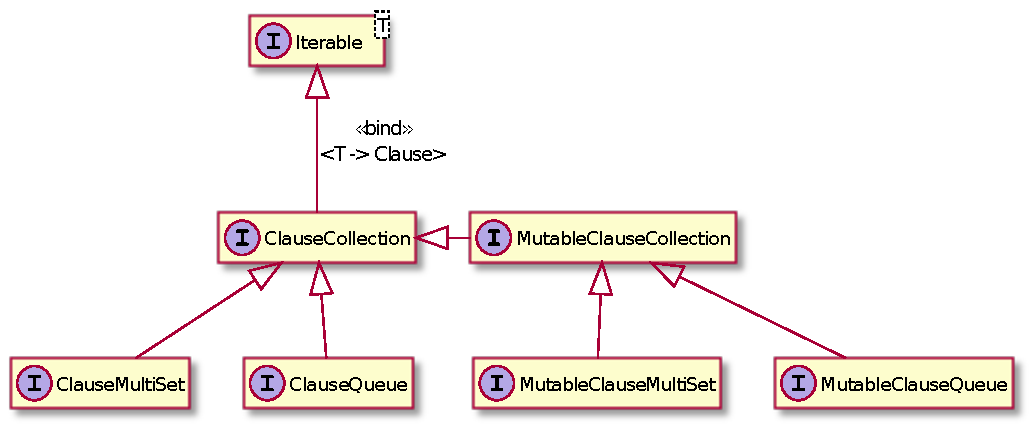
\includegraphics[width=\linewidth]{img/clause-collections.pdf}
    \end{center}

    \framebreak

    \begin{block}{The \kt{ClauseCollection} interface}
        \begin{itemize}
            \item defines typical insertion and removal operations
            \item method names similar to Java Collections
            \begin{itemize}
                \item [!] following the \textit{least astonishment principle}
            \end{itemize}
        \end{itemize}
    \end{block}
    %
    \begin{description}
        \item[\kt{add(Clause): ClauseCollection}] returns a new collection containing the given clause and the existing ones
        \item[\kt{retrieve(Clause): RetrieveResult<ClauseCollection>}] tries to remove the given clause from the collection
        \item[\kt{contains(Clause): Boolean}] checks if the collection contains the given clause
        \item[\kt{size: Int}] computes the size of the collection
        \item[\kt{isEmpty(): Boolean}] checks if the collection contains any clauses 
        \item[\kt{iterator(): Iterator<Clause>}] returns the collection's iterator
    \end{description}

    \framebreak

    \begin{block}{The \kt{RetrieveResult} type}
        \begin{itemize}
            \item represents the output of a \kt{retrieve(Clause)} call
            \item can be a \kt{Success} or \kt{Failure}
        \end{itemize}
    \end{block}
    %
    \begin{center}
        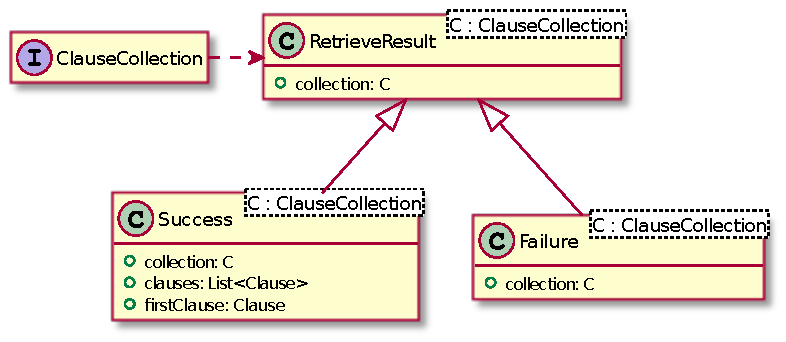
\includegraphics[width=0.8\linewidth]{img/retrieve-result.pdf}
    \end{center}

    \framebreak

    \begin{block}{The \kt{MutableClauseCollection} interface}
        \begin{itemize}
            \item subtype of \kt{ClauseCollection}
            \item insertions and removals are performed \textbf{in-place}
            \begin{description}
                \item [!] same collection is returned after any operation
            \end{description}    
        \end{itemize}
    \end{block}
    %
    \begin{description}
        \item [\kt{add(Clause): MutableClauseCollection}] adds a new clause to this collection
        \item [\kt{retrieve(Clause): RetrieveResult<MutableClauseCollection>}] tries to remove the given clause from this collection
    \end{description}

    \framebreak

    \begin{block}{Clause Queues}
        \begin{itemize}
            \item \textbf{preserve} the \textbf{ordering} of clauses
            \begin{description}
                \item [!] according to their \textit{insertion} order
            \end{description}
            \item store clauses in a \textit{queue}-like structure
            \item defined by the \kt{ClauseQueue} and \kt{MutableClauseQueue} types
        \end{itemize}
    \end{block}
    %
    \begin{description}
        \item[\kt{addFirst(Clause): ClauseQueue}] adds a clause in the \textit{first} position to the collection
        \item[\kt{add/addLast(Clause): ClauseQueue}]  adds a clause in the \textit{last} position to the collection 
        \item[\kt{getFifoOrdered(Clause): Sequence<Clause>}] produces a sequence of clauses unifying with the given one, searching \textit{from first to last}
        \item[\kt{getLifoOrdered(Clause): Sequence<Clause>}] produces a sequence of clauses unifying with the given one, searching \textit{from last to first}
    \end{description}

    \framebreak

    \begin{block}{Clause Multisets}
        \begin{itemize}
            \item ignore clause ordering
            \item useful when many clauses may match the goal
            \item defined by the \kt{ClauseMultiSet} and \kt{MutableClauseMultiSet} types
        \end{itemize}
    \end{block}
    %
    \begin{description}
        \item[\kt{count(Clause): Long}] computes the number of clauses unifying with the given one
        \item[\kt{get(Clause): Sequence<Clause>}] produces a sequence of clauses that unify with the given one
        \begin{description}
            \item[!] equivalent to the \kt{[]} operator
        \end{description}
    \end{description}

\end{frame}

\begin{frame}[allowframebreaks]{Creating \kt{ClauseCollection}s}
    Main \kt{ClauseCollection} static factories:
    %
    \begin{description}
        \item[\kt{emptyMultiSet(): ClauseMultiSet}] creates an empty \kt{ClauseMultiset}
        \item[\kt{multiSetOf(Iterable<Clause>): ClauseMultiSet}] creates a \kt{ClauseMultiSet} from the given clauses
        \item[\kt{emptyQueue(): ClauseQueue}] creates an empty \kt{ClauseQueue}
        \item[\kt{queueOf(Iterable<Clause>): ClauseQueue}] creates a \kt{ClauseQueue} from the given clauses
    \end{description}
    %
    These factories return \textit{immutable} collections by default

    \framebreak

    \kt{ClauseQueue} and \kt{ClauseMultiSet} provide three main static factories:
    %
    \begin{description}
        \item[\kt{empty()}: C] creates an empty \kt{C}
        \item[\kt{of(Iterable<Clause>)}: C] creates a \kt{C} from the given clauses
        \item[\kt{of(vararg Clause)}: C] creates a \kt{C} from the given clauses
    \end{description}
    %
    with \kt{C} being either \kt{ClauseQueue} or \kt{ClauseMultiSet}
\end{frame}

\begin{frame}[allowframebreaks]{Using \kt{ClauseCollection}s}
    Ordering a \kt{ClauseQueue}:
    %
    \ktSnippet{./snippets/QueueOrdering.kt}

    \framebreak

    Populating a \kt{ClauseQueue}:
    %
    \ktSnippet{./snippets/QueuePopulate.kt}

    \framebreak

    Retrieving clauses from a \kt{ClauseQueue}:
    %
    \ktSnippet{./snippets/QueueRetrieve.kt}

    \framebreak

    Working with \kt{ClauseMultiSet}s:
    %
    \ktSnippet{./snippets/MultiSet.kt}
\end{frame}

\subsection{Theories}

\begin{frame}[allowframebreaks]{Theories Design and Implementations}

    \begin{block}{The \kt{Theory} type}
        \begin{itemize}
            \item provides high-level management of \kt{Clause}s
            \item meant as a \textit{façade} through which client code can access a knowledge base
            \item design and implementation mirror the ones devised for \kt{Clause} collections
            \item designed as \kt{Iterable} sub-types
        \end{itemize}
    \end{block}
    
    \framebreak

    \begin{block}{Mutable vs. immutable theories}
        Just like \kt{ClauseCollection}s,
        %
        \begin{itemize}
            \item \textit{mutable} theories can be modified in place
            \item \textit{immutable} theories cannot be changed: their operations build new ones containing the modified clauses
        \end{itemize}
    \end{block}
    %
    \begin{block}{Indexed vs. listed Theories}
        Theories come into two main implementations:
        \begin{itemize}
            \item \textit{indexed} theories are backed by an indexed data structure
            \begin{description}
                \item [!] providing faster look-up, but taking up more space
            \end{description}
            \item \textit{list-based} theories are backed by lists
            \begin{description}
                \item [!] slower but memory-efficient
                \item [!] preserve order of \kt{Clause}s
            \end{description}
        \end{itemize}
    \end{block}

\end{frame}

\begin{frame}[allowframebreaks]{The \kt{Theory} Type Hierarchy}

    \begin{center}
        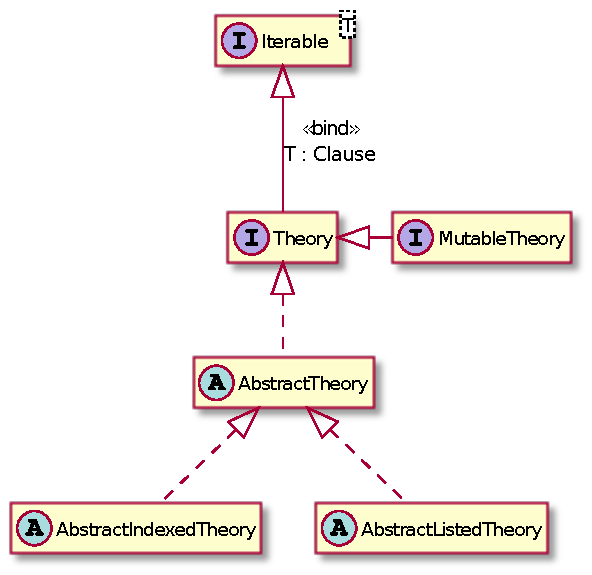
\includegraphics[width=0.6\linewidth]{img/theory-base.pdf}
    \end{center}

    \framebreak

    \begin{center}
        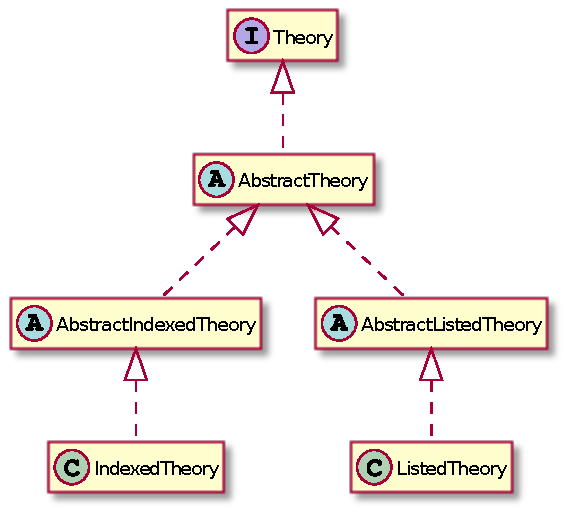
\includegraphics[width=0.6\linewidth]{img/theory-immutable.pdf}
    \end{center}

    \framebreak

    \begin{center}
        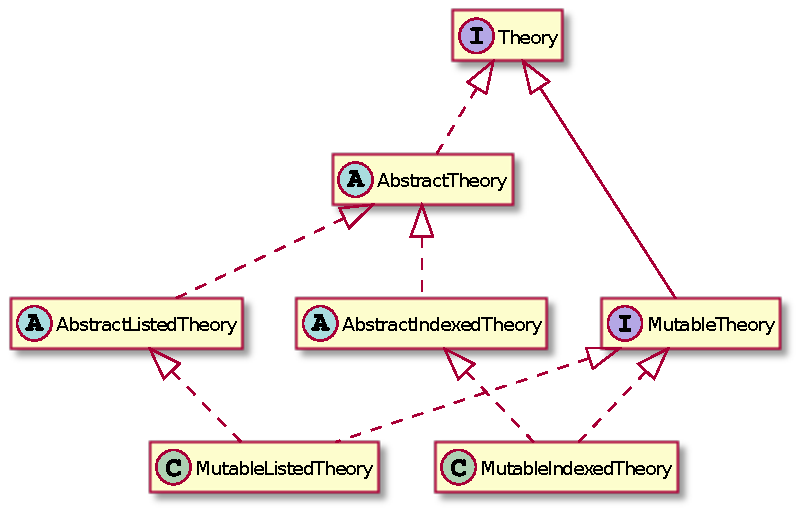
\includegraphics[width=0.7\linewidth]{img/theory-mutable.pdf}
    \end{center}

    \framebreak

    Main \kt{Theory} methods:
    \begin{description}
        \item[\kt{assertA(Clause): Theory}] adds the given clause \textit{before} all other clauses in this theory
        \item[\kt{assertZ(Clause): Theory}] adds the given clause \textit{after} all other clauses in this theory
        \item[\kt{abolish(Indicator): Theory}] removes all the clauses matching the given \kt{Indicator}
        \item[\kt{retract(Clause): RetractResult<Theory>}] tries to delete a matching clause from this theory
    \end{description}

    \framebreak

    \begin{description}
        \item[\kt{plus(Theory): Theory}] adds the given \kt{Theory} to this
        \item[\kt{contains(Clause): Boolean}] checks if the given \kt{Clause} is contained in this \kt{Theory}
        \item[\kt{get(Clause): Sequence<Clause>}] retrieves all matching clauses from this \kt{Theory}
        \item[\kt{toMutableTheory(): MutableTheory}] converts this \kt{Theory} to a mutable one
        \item[\kt{toImmutableTheory(): Theory}] converts this \kt{Theory} to an immutable one
    \end{description}

    \framebreak
    
    \begin{block}{The \kt{RetractResult} type}
        \begin{itemize}
            \item represents the output of a \kt{retract(Clause)} call
            \item can be a \kt{Success} or a \kt{Failure}
        \end{itemize}
    \end{block}
    %
    \begin{center}
        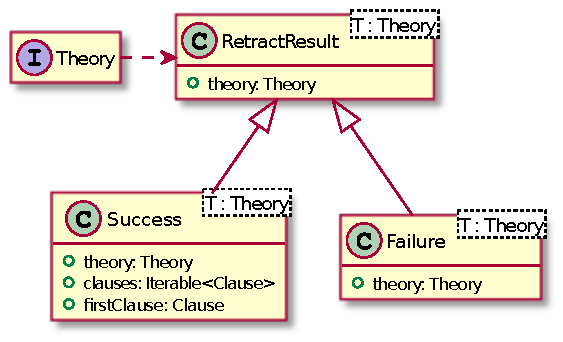
\includegraphics[width=0.7\linewidth]{img/retract-result.pdf}
    \end{center}    

\end{frame}

\begin{frame}[allowframebreaks]{Creating a \kt{Theory}}
    Static factories for \kt{Theory} (same methods apply for \kt{MutableTheory}):
    %
    \begin{description}
        \item[\kt{empty(): Theory}] creates an empty \kt{Theory} (indexed by default)
        \item[\kt{of(vararg Clause): Theory}] creates a \kt{Theory} containing the given clauses
        \item[\kt{emptyIndexed(): Theory}] creates an empty \kt{Theory} backed by an indexed data structure
        \item[\kt{indexedOf(vararg Clause): Theory}] creates an indexed \kt{Theory} containing the given \kt{Clauses} 
        \item[\kt{emptyListed(): Theory}] creates an empty \kt{Theory} backed by a list
        \item[\kt{listedOf(vararg Clause): Theory}] creates a \kt{Theory} backed by a list, containing the given clauses
    \end{description}
\end{frame}

\begin{frame}[allowframebreaks]{Using a \kt{Theory}}
    Asserting clauses into a \kt{Theory}:
    %
    \ktSnippet{./snippets/TheoryAssert.kt}

    \framebreak

    Abolishing \kt{Indicator}s from a \kt{Theory}:
    %
    \ktSnippet{./snippets/TheoryAbolish.kt}

    \framebreak

    Retracting clauses from a \kt{Theory}:
    %
    \ktSnippet{./snippets/TheoryRetract.kt}
\end{frame}

\section{Generic Logic Resolution: the \module{solve} Module}

\begin{frame}[allowframebreaks]{The \module{solve} Module: Overview}

    \begin{block}{Purpose}
        \begin{itemize}
            \item Provide generic support to logic resolution
            \item Re-use as much as possible of Prolog standard 
            %
            \begin{itemize}
                \item without committing to any particular resolution strategy
                \item nor to any inference procedure
            \end{itemize}
        \end{itemize}
    \end{block}

    \framebreak

    Thus, \module{solve} provides the following abstractions:

    \begin{block}{Solvers and Solutions}\centering
        Solvers are reactive entities capable of answering to users' queries by producing one or more solutions, exploiting logic resolution
    \end{block}

    \begin{block}{Execution Contexts}
        \begin{center}
            An execution context encapsulates some solver's internal state.
            Resolution affects and is affected by the solver's execution context.
        \end{center}

        \small
        Composed by:
        %
        \begin{description}
            \item[libraries] | containers of built-in functionalities exploitable by resolution
            \item[flags] | configurable aspects of a solver
            \item[knowledge bases] (KB) | containers of the logic knowledge used by resolution
            \item[operators] | set of operators used to parse queries and to present solutions
            \item[channels] | I/O facilities to communicate with the external world
        \end{description}
        %
        \begin{itemize}\small
            \item[+] any resolution-specific aspect
            %
            \begin{itemize}\scriptsize
                \item (this may vary depending on how resolution is implemented)
            \end{itemize} 
        \end{itemize}
    \end{block}

    \framebreak

    \begin{block}{Libraries}
        \begin{center}
            Containers of built-in functionalities exploitable by resolution
        \end{center}
        
        Possibly, including:
        %
        \begin{description}
            \item[some \textbf{clauses}] containing logic predicates provided by the library
            \item[some \textbf{primitives}] i.e., logic predicates, implemented in Kotlin, and provided by the library
            \item[some \textbf{functions}] i.e., custom ways to reduce expressions of terms
            \item[some \textbf{operators}] automatically imported into the solver along with the library 
        \end{description}
    \end{block}

    \framebreak

    \begin{block}{Flags}
        \begin{center}
            Key-value pairs aimed at configuring a solver behaviour
        \end{center}
        
        Where:
        %
        \begin{itemize}
            \item the key is a string
            \item the value is an arbitrary term
        \end{itemize}
    \end{block}

    \framebreak

    \begin{block}{Knowledge bases (KB)}
        \begin{center}
            Containers of the logic knowledge taken into account by resolution to answer users' queries
        \end{center}
        
        Following Prolog's conventions, KB are of two sorts:
        %
        \begin{description}
            \item[static KB] | which cannot be altered during resultion
            \item[dynamic KB] | which can be altered during resultion 
        \end{description}
    \end{block}

    \framebreak

    \begin{block}{Operators}
        \begin{center}
            Each solver may operate upon a dynamic set of operators
        \end{center}
        
        That:
        %
        \begin{itemize}
            \item may be loaded along with libraries or be dynamically altered during resolution
            \item may affect the way users' queries are parsed
            \item may affect the way solutions are presented to users
        \end{itemize}
    \end{block}

    \framebreak

    \begin{block}{Channels}
        \begin{center}
            Communication facilities among the solver and the external world
        \end{center}
        
        Channels are of two sorts:
        %
        \begin{description}
            \item[input channels] (a.k.a. \alert{sources}) let a solver receive inputs messages
            \item[output channels] (a.k.a. \alert{sinks}) let a solver provide output messages
        \end{description}
    \end{block}
\end{frame}

\subsection{\kt{Solver}s and the \kt{Solution}s}

\begin{frame}[allowframebreaks]{The \kt{Solver}, \kt{Solution}, and \kt{SolveOptions} Types}
    % Solver

    % MutableSolver

    % Solution.*

    % SolveOpts

    \begin{center}
        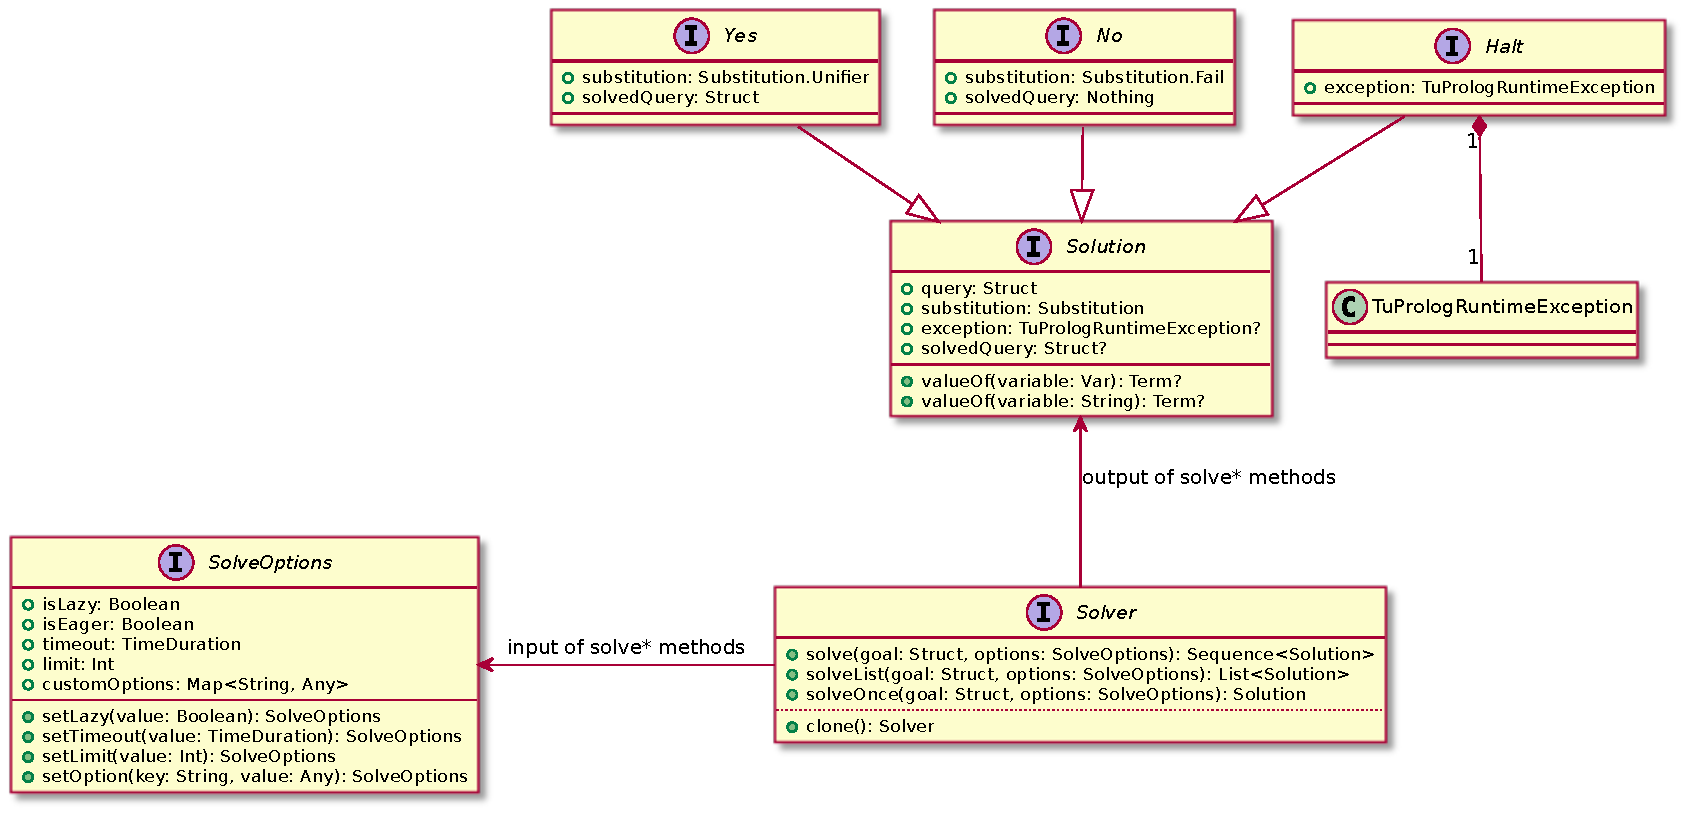
\includegraphics[width=\linewidth]{img/solve-io.pdf}
    \end{center}

    \begin{block}{The \kt{Solver} type}
        \kt{Solver}s expose many \kt{solve*} methods, accepting:
        %
        \begin{itemize}
            \item a \alert{goal}, i.e. a \kt{Struct} representing the query to be answered via resolution
            \item an instance of \kt{SolveOptions} describing/constraining the way answers are provided
        \end{itemize}
        %
        and returning one or more \kt{Solution}s 
    \end{block}

    \begin{block}{The \kt{Solution} type}
        A \kt{Solution} represents an answer provided by a \kt{Solver} w.r.t. the user's query
        It can be of three actual sorts:
        %
        \begin{description}
            \item[\kt{Solution.Yes}] representing a positive answer
            %
            \begin{itemize}\small
                \item carrying a \kt{Unifier} assigning some variable from the user's query
            \end{itemize} 

            \item[\kt{Solution.No}] representing a negative answer

            \item[\kt{Solution.Halt}] representing an exceptional answer
            %
            \begin{itemize}\small
                \item carrying a \kt{TuPrologRuntimeException} locating the error w.r.t. the resultion process
            \end{itemize}
        \end{description}
    \end{block}

    \begin{block}{The \kt{SolveOptions} type}
        Instances of \kt{SolveOptions} are provided along with users' queries and aim at constraining the way solutions are computed by the solver:
        %
        \begin{description}
            \item[\kt{isEager: Boolean}] | if \kt{true} all solutions are computed ASAP
            %
            \begin{itemize}\small
                \item may saturate memory in case of many/infinite solutions!
            \end{itemize} 
            
            \item[\kt{isLazy: Boolean}] | if \kt{true} solutions are \emph{lazily} computed jsut before being consumed
            %
            \begin{itemize}\small
                \item this is \kt{true} by default
            \end{itemize}  

            \item[\kt{timeout: TimeDuration}] | dictates the \alert{maximum} amount of time resolution may use to compute a single solution
            %
            \begin{itemize}\small
                \item defaults to infinite time
            \end{itemize} 
            
            \item[\kt{limit: Int}] | limits the \alert{maximum} amount of computed solutions 
            %
            \begin{itemize}\small
                \item defaults to infinite
            \end{itemize}
        \end{description}
    \end{block}

    \begin{block}{The \kt{solve*} methods in \kt{Solver}}
        \begin{description}
            \item[\kt{solve}] | returns a \kt{Sequence} (i.e., a stream) of \kt{Solution}s
            \item[\kt{solveList}] | returns a \kt{List} of \kt{Solution}s 
            %
            \begin{itemize}\small
                \item implies \kt{solveOpts.isEager == true}
            \end{itemize} 
            \item[\kt{solveOnce}] | returns a single \kt{Solution} 
            %
            \begin{itemize}\small
                \item implies \kt{solveOpts.limit == 1}
            \end{itemize} 
        \end{description}
    \end{block}

    \framebreak

    \ktSnippet{./snippets/MissingExample.kt}

\end{frame}

\begin{frame}[allowframebreaks]{\kt{Solver} vs. \kt{MutableSolver}}
    Notice that there are 2 types for solvers:
    %
    \begin{center}
        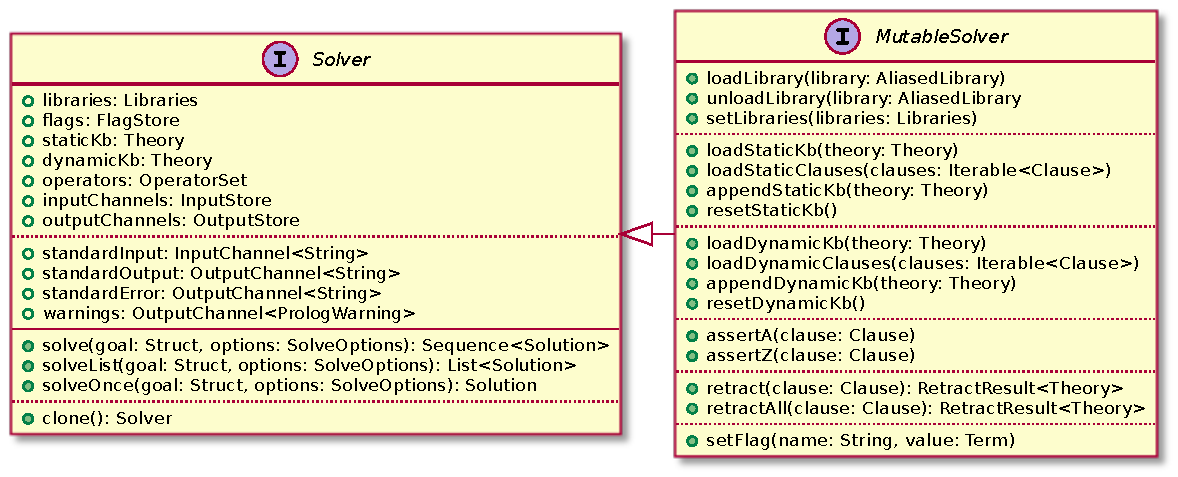
\includegraphics[width=.8\linewidth]{img/solve-mutable.pdf}
    \end{center}
    %
    \begin{itemize}\small
        \item \emph{solvers} expose properties supporting \alert{inspection} of their state
        \item \alert{mutable} solvers expose methods to \alert{alter} their state
        %
        \begin{itemize}
            \item[!] the state of \emph{non}-mutable solvers may change too, because of resolution
            %
            \begin{itemize}
                \item[$\rightarrow$] they are \alert{not} immutable
            \end{itemize} 
        \end{itemize}
    \end{itemize}
\end{frame}

\begin{frame}[allowframebreaks]{Creating \kt{Solvers} via a \kt{SolverFactory}}
    \begin{block}{About solver factories}\centering
        Objects of type \kt{SolverFactory} aim at instantiating \kt{Solver}s
    \end{block}

    \bigskip

    Main sorts of methods:
    %
    \begin{description}
        \item[\kt{solverOf(\ldots)}] | creates an empty \kt{Solver}
        \item[\kt{solverWithDefaultBuiltins(\ldots)}] | creates a \kt{Solver} and endows it with some default built-in predicates
        \item[\kt{mutableSolverOf(\ldots)}] | creates an empty \kt{MutableSolver}
        \item[\kt{mutableSolverWithDefaultBuiltins(\ldots)}] | creates a \kt{MutableSolver} and endows it with some default built-in predicates
    \end{description}

    \framebreak
    
    \begin{itemize}
        \item All such methods come with various overloads\ldots
        \item \ldots letting the caller specify the new solver's:
        %
        \begin{enumerate}
            \item libraries to be loaded upon construction 
            %
            \begin{itemize}
                \item (possibly, other than the default ones)
            \end{itemize}
            \item initial values of specific flags
            \item content of the static KB
            \item initial content of the dynamic KB
            \item operators to be loaded upon construction
            \item input/output channels to be used for the solver
            \item or some sub-set of the above
        \end{enumerate}
    \end{itemize}

    \framebreak

    \begin{alertblock}{Important convention}\centering
        All implementations of \kt{Solver} should be packed with a corresponding implementation of \kt{SolveFactory}, possibly as a \alert{singleton}
    \end{alertblock}
    %
    \begin{itemize}
        \item[eg] \module{solve-classic} exposes object \kt{ClassicSolverFactory}
        %
        \begin{itemize}
            \item also accessbile via \kt{Solver.\alert{classic}}
        \end{itemize} 

        \item[eg] \module{solve-streams} exposes object \kt{StreamsSolverFactory}
        %
        \begin{itemize}
            \item also accessbile via \kt{Solver.\alert{streams}}
        \end{itemize} 
    \end{itemize}

    \framebreak

    \ktSnippet{./snippets/MissingExample.kt}

\end{frame}

\begin{frame}[allowframebreaks]{Using a \kt{Solver}}

    \begin{block}{Concept}
        \centering
        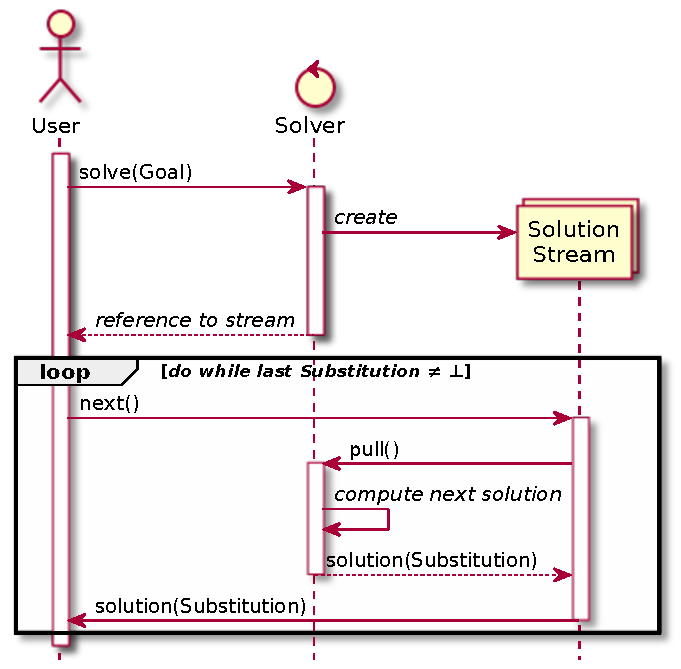
\includegraphics[width=.4\linewidth]{img/streamful-solver.pdf}
    \end{block}

    \framebreak

    \ktSnippet{./snippets/MissingExample.kt}
\end{frame}

\subsection{The \kt{ExecutionContext}}

\begin{frame}[allowframebreaks]{Overview on the general purpose \kt{ExecutionContext}}
    \begin{itemize}
        \item Module \module{solve} exposes a general interface for \kt{ExecutionContext}s
        \item This must be exploited \& customised by implementers of \kt{Solver}s
    \end{itemize}
    %
    \begin{center}
        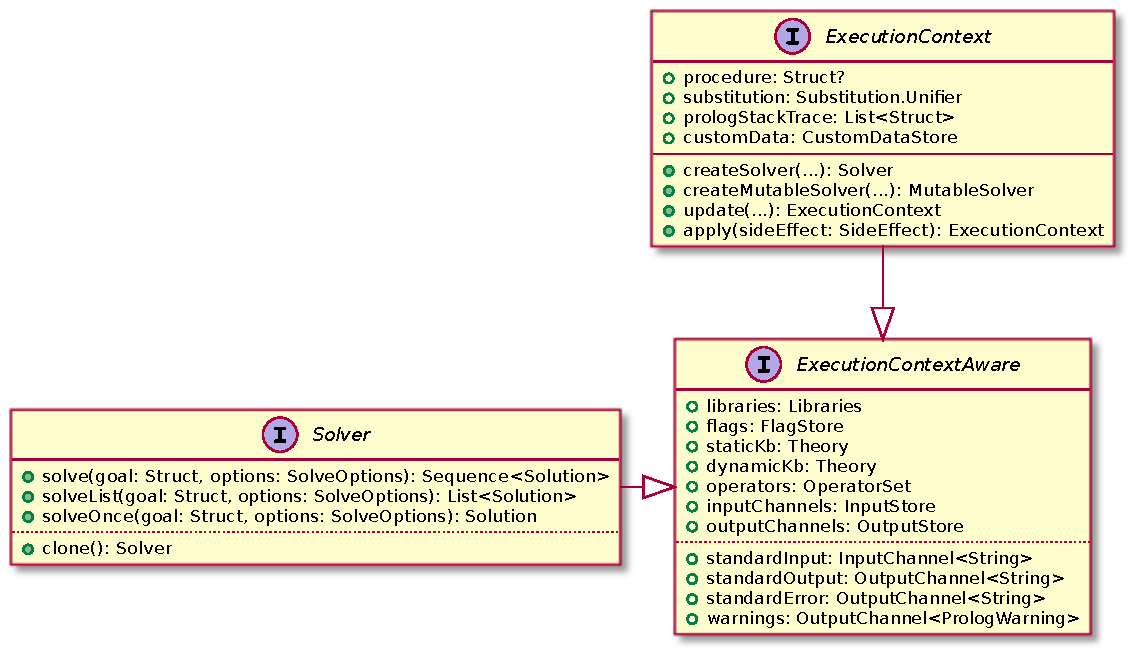
\includegraphics[width=.6\linewidth]{img/solve-ec.pdf}
    \end{center}

    \framebreak

    \begin{block}{An \kt{ExecutionContext} keeps track of (at least)}
        \begin{itemize}
            \item all inspectable aspects of a \kt{Solver}
            %
            \begin{itemize}
                \item[ie] libraries, flags, KB, operators, and channels
            \end{itemize}
            \item[+] the \alert{\kt{procedure}} resolution is currently focussing upon
            \item[+] the \alert{\kt{substitution}} resolution has constructed so far 
            \item[+] other fields possibly specified/customised by implementers
        \end{itemize}
    \end{block}

    \framebreak

    \begin{alertblock}{Conventions}
        \begin{itemize}
            \item \kt{ExecutionContext}s are \alert{immutable}
            
            \item An \kt{ExecutionContext} can be attained from another one via:
            %
            \begin{description}\small
                \item[\kt{update(\ldots)}] | creating a copy of the current context, only differing for the provided fields
                \item[\kt{apply(\textit{SideEffect})}] | creating a copy of the current context by applying the provide \kt{SideEffect} to it
            \end{description}
        \end{itemize}
    \end{alertblock}

    \framebreak

    \begin{exampleblock}{Notice that}
        \begin{itemize}
            \item It is always possible to create a novel \kt{(Mutable)Solver} via
             %
             \begin{description}\small
                \item[\kt{createSolver(\ldots)}] 
                \item[\kt{createMutableSolver(\ldots)}]
            \end{description}

            \item The new solver is initialised using the current context
            %
            \begin{itemize}
                \item[!] this is fundamental to realise complex functionalities
            \end{itemize}
        \end{itemize}
    \end{exampleblock}
\end{frame}

\begin{frame}{\kt{ExecutionContext} is where everything is linked together}
    \centering
    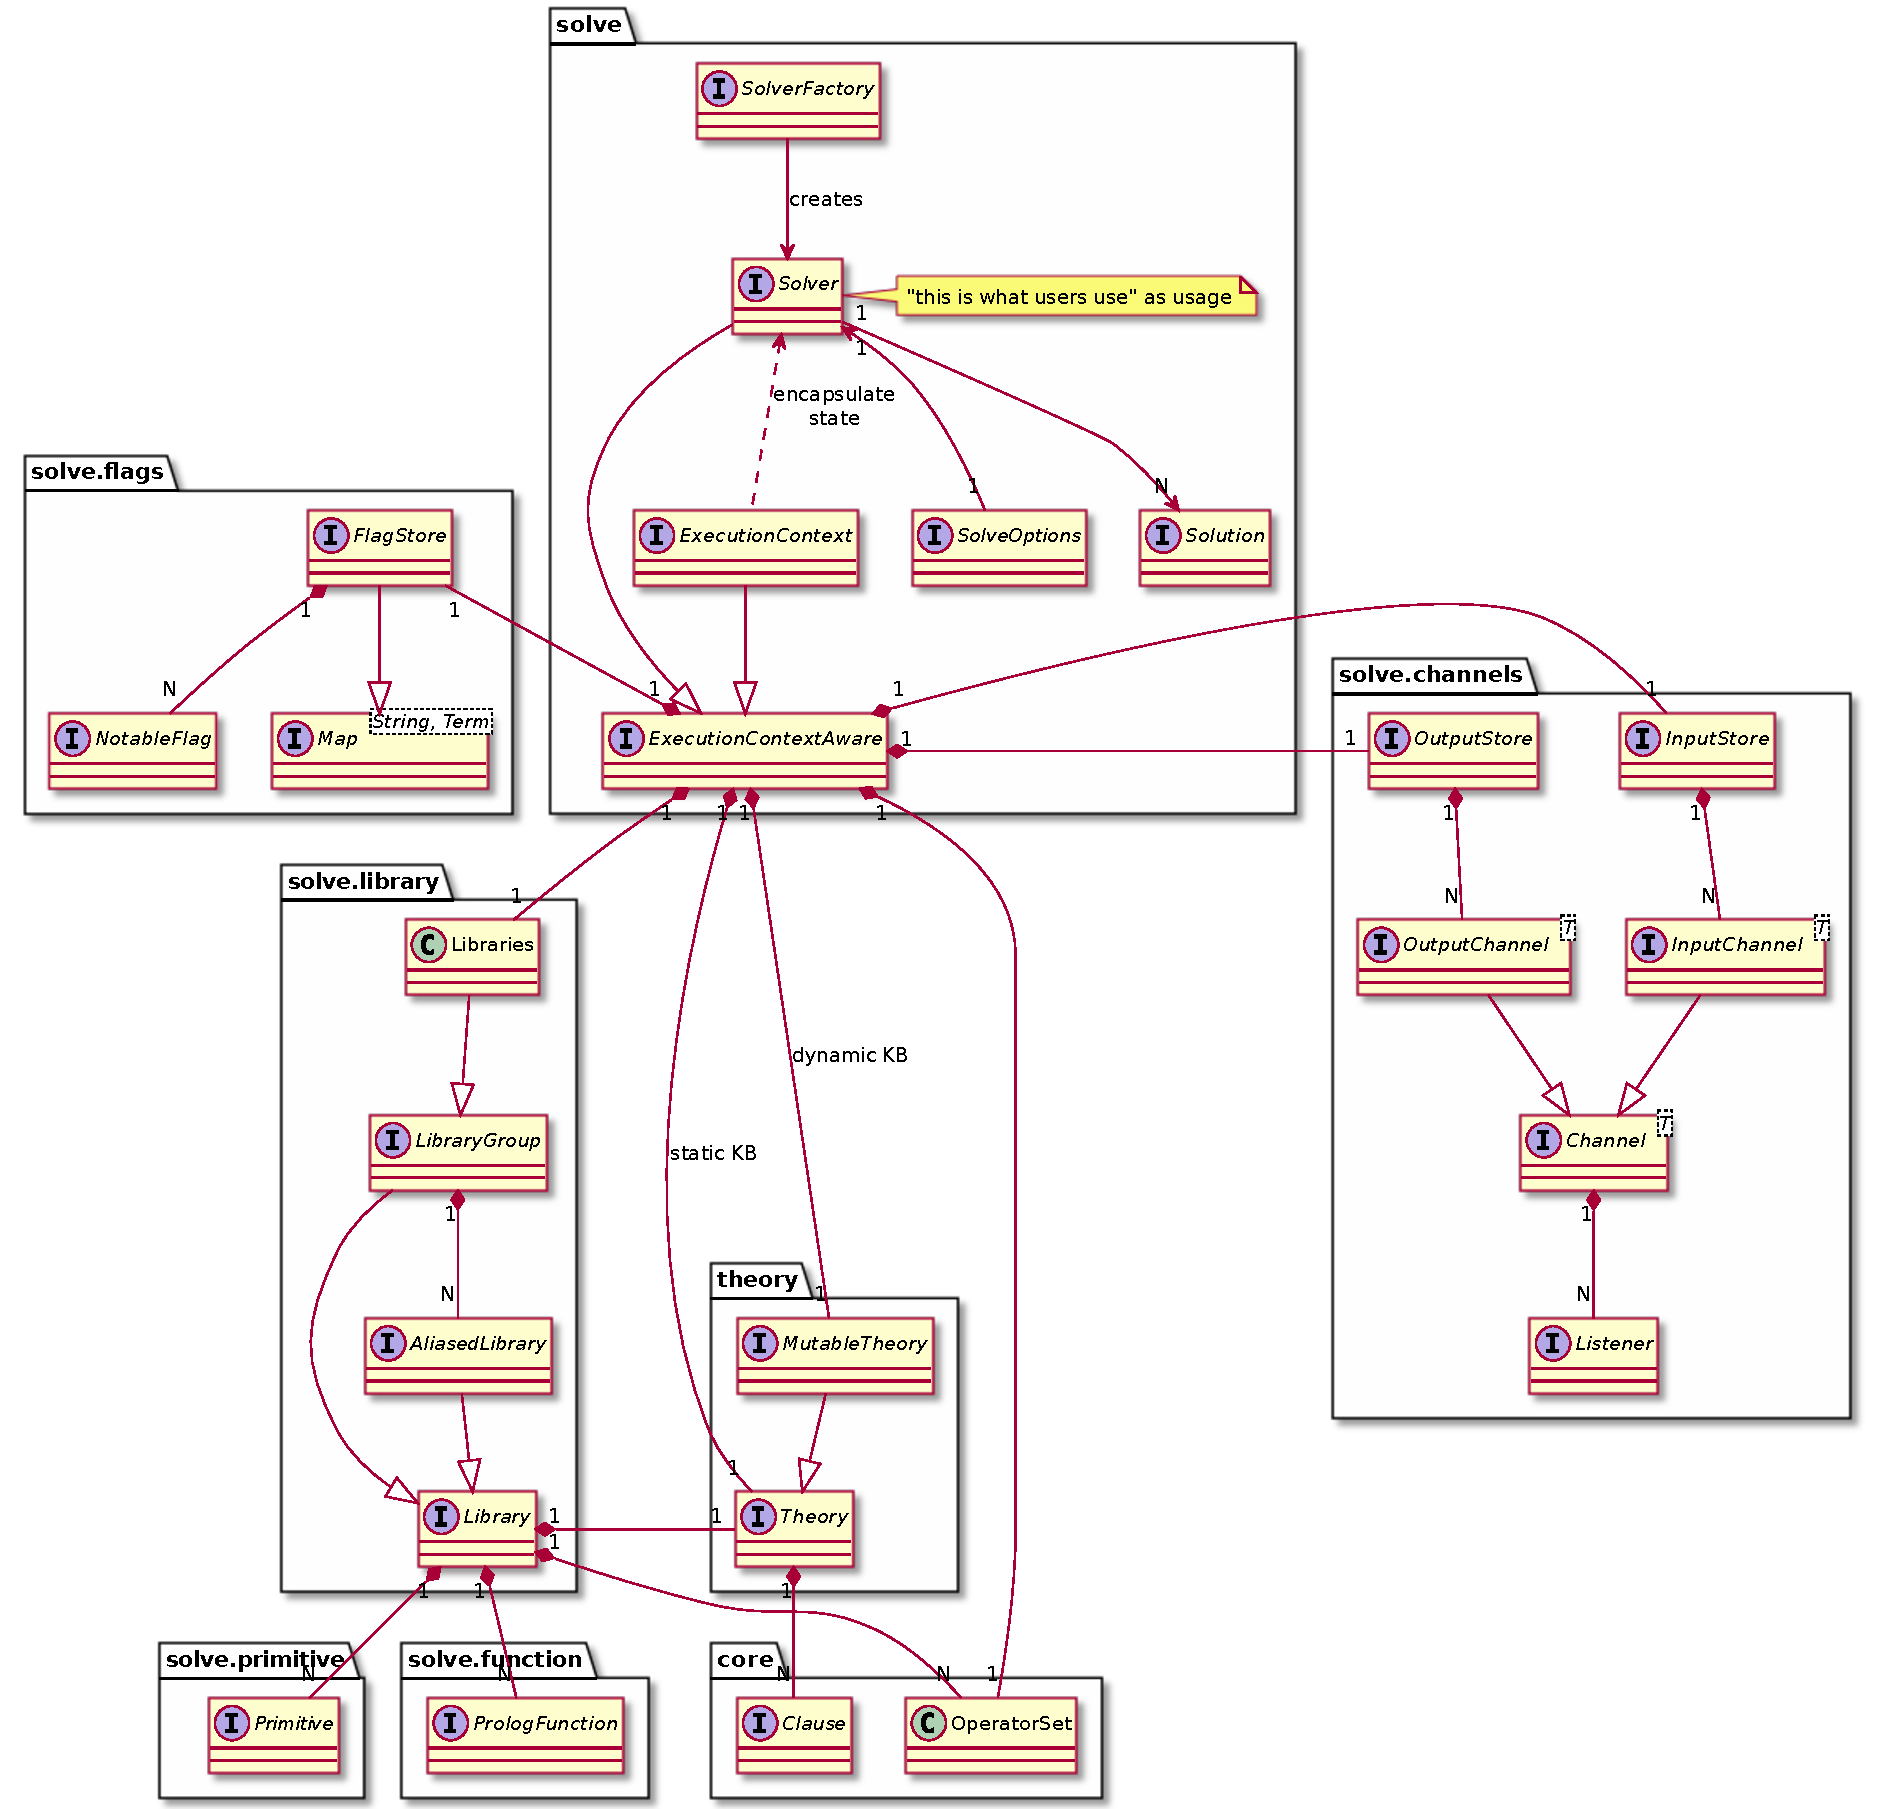
\includegraphics[width=.75\linewidth]{img/solve.pdf}
\end{frame}

\subsubsection{About \kt{Solver}s' Knowledge Bases}

\begin{frame}[allowframebreaks]{Static vs. Dynamic Knowledge bases}
    \begin{alertblock}{Conventions}
        \begin{itemize}
            \item The \kt{staticKb} is assumed to reference an \alert{immutable} \kt{Theory}
            %
            \begin{itemize}
                \item[ie] read efficient
            \end{itemize}

            \item The \kt{dynamicKb} is assumed to reference a \kt{\alert{Mutable}Theory}
            %
            \begin{itemize}
                \item[ie] write efficient
            \end{itemize}

            \item Resolution is generally only allowed to alter the \alert{dynamic} KB
            %
            \begin{itemize}
                \item[eg] via \pl{assert/1}, or \pl{retract/1}
            \end{itemize}

            \item However, notable exceptions exist
            %
            \begin{itemize}
                \item[eg] via \pl{consult/1}, or \pl{register/2} (from the \module{oop-lib} module)
            \end{itemize}
        \end{itemize}
    \end{alertblock}
\end{frame}

\begin{frame}[allowframebreaks]{Example: Using \kt{Solver}s with custom KB}

    \begin{block}{Endowing \kt{Solver}s with their KB}
        \begin{itemize}
            \item \kt{Solver}s can be provided with their KB upon construction
            %
            \begin{itemize}
                \item cf. \kt{SolverFactory}'s methods
            \end{itemize}

            \item \kt{MutableSolver}s can be provided with their KB dynamically
            %
            \begin{itemize}
                \item[eg] via the many methods of \kt{MutableSolver}
            \end{itemize}
        \end{itemize}
    \end{block}

    \framebreak

    \ktSnippet{./snippets/MissingExample.kt}
    % initialising a solver with custom knowledge bases

    \framebreak

    \ktSnippet{./snippets/MissingExample.kt}
    % loading a custom kb into a mutable solver
\end{frame}

\begin{frame}[allowframebreaks]{Custom KB and \kt{Directive}s}

    \begin{block}{About directives}
        \begin{itemize}
            \item KB may contain some \kt{Directive}s
            \item Implementations of \kt{Solver} should react to particular \kt{Directive}s
            %
            \begin{itemize}
                \item upon KB provisioing (either by construciton or otherwise)
                \item other sorts of directives are ignored
            \end{itemize}
            \item Notice that \kt{Directive}s are just headless \kt{Clauses}
            %
            \begin{itemize}
                \item unless they are provided to a \kt{Solver}
                \item at that point, they acquire procedural meaning
            \end{itemize}
        \end{itemize}
    \end{block}

    \framebreak

    Notable directives:
    %
    \begin{description}
        \item[\pl{:- dynamic(\textit{F} / \textit{N}).}] makes any subsequent clause whose head indicator is \pl{\textit{F}/\textit{N}} be loaded into the \alert{dynamic} KB, event if the theory is loaded as static
        \item[\pl{:- static(\textit{F} / \textit{N}).}] dual w.r.t. \pl{dynamic(F/N)}
        \item[\pl{:- op(\textit{P}, \textit{S}, \textit{F}).}] loads a new operator into the \kt{Solver}, having the provided proprity (\pl{\textit{P}}), specifier (\pl{\textit{S}}), and functor (\pl{\textit{F}})
        \item[\pl{:- solve(\textit{G}).}] executes goal \pl{\textit{G}} as soon as the theory has been loaded
        \item[\pl{:- initialization(\textit{G}).}] alias for \pl{solve(\textit{G})}
        \item[\pl{:- set\_prolog\_flag(\textit{N}, \textit{V}).}] (re)sets the flag named \pl{\textit{N}} to the value \pl{\textit{V}}
        \item[\pl{:- include(\textit{P}).}] loads the theory whose path is \pl{\textit{P}} as if it was part of the currently loading one
        %
        \begin{itemize}\small
            \item[!] requires the \module{io-lib} module to be available at run-time 
        \end{itemize} 
        \item[\pl{:- load(\textit{P}).}] alias for \pl{include(\textit{P})} 
    \end{description}

    \framebreak

    \ktSnippet{./snippets/MissingExample.kt}
\end{frame}

\subsubsection{Extending \kt{Solver}s via \kt{Libraries}}

\begin{frame}[allowframebreaks]{Overview on \kt{Libraries}}
    \begin{block}{Why \kt{Libraries}}
        \begin{itemize}
            \item Need to extend \kt{Solver}s via built-in functionalities
            \item[eg] operators, rules, (logic) functions, or primitives
        \end{itemize}
    \end{block}

    \framebreak

    \begin{center}
        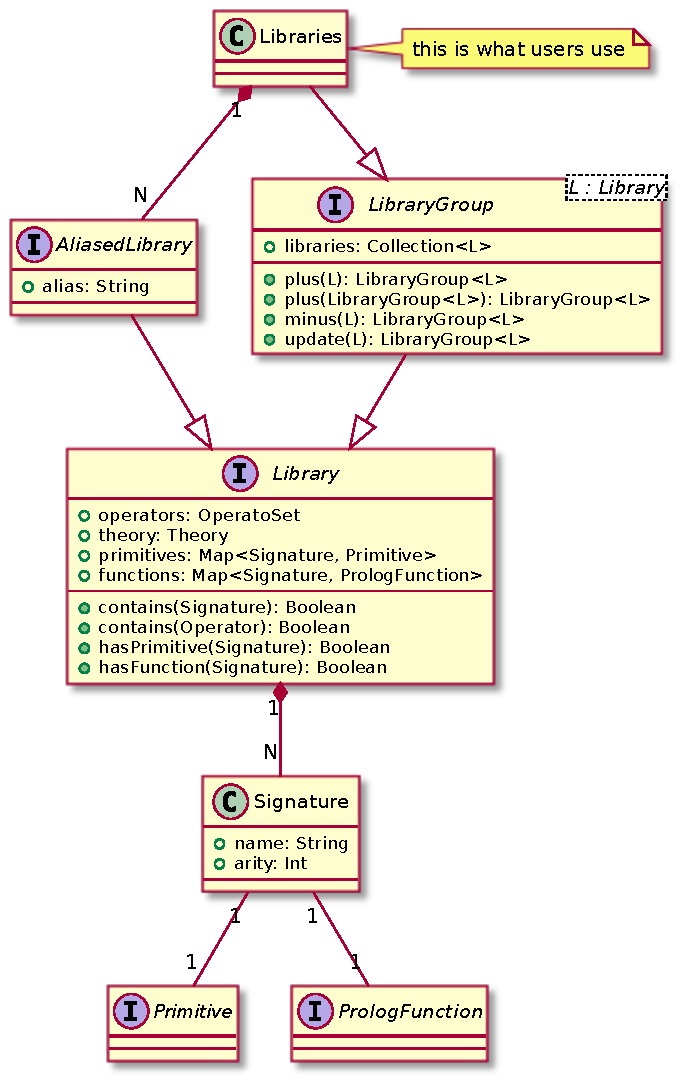
\includegraphics[height=.75\textheight]{img/libraries.pdf}
    \end{center}

    \framebreak

    \begin{block}{Definition: \kt{Library}}
        A type for \alert{immutable} containers of:
        %
        \begin{description}
            \item[operators] to be loaded along with the \kt{Library}
            \item[theory] in turn containing pre-built rules and facts
            \item[primitives] i.e. logic predicates, written in Kotlin
            \item[functions] i.e. logic functions, written in Kotlin 
        \end{description}
    \end{block}

    \begin{block}{Definition: \kt{Signature}}
        Primitives and functions are indexed in \kt{Library}s via \kt{Signature}s,
        %
        \begin{itemize}
            \item[ie] \kt{name}-\kt{arity} pairs
        \end{itemize}
    \end{block}

    \framebreak

    \begin{block}{Definition: \kt{AliasedLibrary}}
        A \kt{Library} with an \alert{alias}
        %
        \begin{itemize}
            \item think about aliases as Java packages names
        \end{itemize}
    \end{block}

    \begin{exampleblock}{Conventions on \textbf{aliases}}
        \begin{itemize}
            \item Same of Jiesava packages names
            \item[ie] camel case, dot separated, spaceless
            \item[eg] \texttt{prolog.lang}, \texttt{prolog.io} 
        \end{itemize}
    \end{exampleblock}

    \framebreak

    \begin{block}{Definition: \kt{LibraryGroup}}
        A \kt{Library} attained by collecting several \kt{Library}s
    \end{block}

    \framebreak

    \begin{block}{Definition: \kt{Libraries}}
        A group of \kt{AliasedLibrary}, indexed by \alert{alias} 
    \end{block}
    %
    \begin{itemize}
        \item this is what \kt{Solver}s' users use, in practice
    \end{itemize}

    \framebreak

    \ktSnippet{snippets/MissingExample.kt}

\end{frame}

\begin{frame}[allowframebreaks]{The \kt{Primitive} Type}

    \begin{alertblock}{Problem}
        \begin{itemize}
            \item Some built-in logic functionalities are easier to write in Kotlin
            \item \ldots as they require \alert{altering} the \kt{Solver}'s \kt{ExecutionContext}
            %
            \begin{itemize}
                \item[eg] \pl{assert/1}, \pl{retract/1}, \pl{write/1}
            \end{itemize}
            \item Some logic functionalities may exploit external computational facilities
        \end{itemize}
    \end{alertblock}

    \begin{block}{Why \kt{Primitive}s}
        \begin{itemize}
            \item A means for calling Kotlin code from LP
            \item A means for writing logic \alert{relations} via OOP+FP+IP
        \end{itemize}
    \end{block}

    \framebreak

    Client-server metaphor:
    %
    \begin{itemize}
        \item users are clients for \kt{Solver}s, which act as servers
        \item \kt{Solver}s are clients for \kt{Primitive}s, which act as servers
    \end{itemize}

    \smallskip

    \begin{center}
        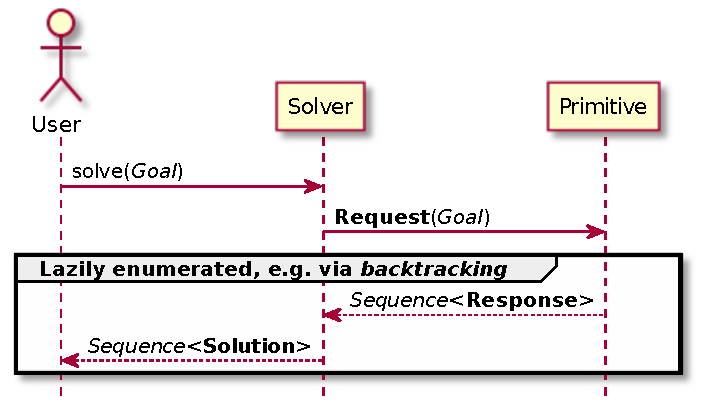
\includegraphics[width=.5\linewidth]{img/primitive-usage.pdf}
    \end{center}

    \framebreak
    
    When needing to solve a (sub-)goal $G$, a \kt{Solver} may
    %
    \begin{itemize}
        \item look into its KB, or
        \item pick a \kt{Primitive} $P$, compliant with $G$, from a \kt{Library}
        %
        \begin{enumerate}
            \item send a \alert{request}, describing $G$, to $P$
            \item receive several \alert{responses}, describing solutions to $G$, from $P$
            %
            \begin{itemize}
                \item possibly containing some \emph{side effect}, to be \alert{reified}
            \end{itemize}
        \end{enumerate}
    \end{itemize}

    \framebreak

    In code:
    %
    \begin{center}
        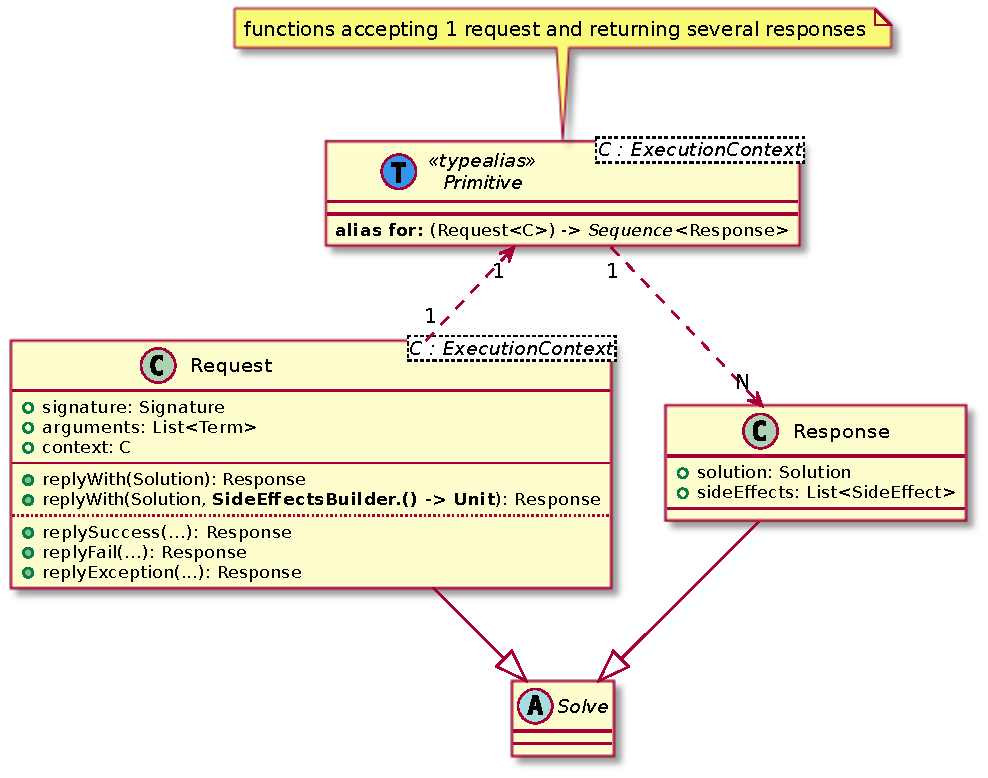
\includegraphics[width=.5\linewidth]{img/primitive.pdf}
    \end{center}

    \framebreak

    \ktSnippet{snippets/MissingExample.kt}
    % sum (functional)

    \ktSnippet{snippets/MissingExample.kt}
    % natural (backtraclabkle)

    \framebreak

    \begin{block}{The many sides of the \kt{Primitive}s}
        \kt{Primitive} are:
        %
        \begin{itemize}
            \item $N$-ary relations, in the eyes of LP
            \item servers \& data producers, in the eyes of \kt{Solver}s
            \item callbacks, in the eyes of libraries implementers
        \end{itemize}
    \end{block}

    \framebreak

    \begin{block}{Within \kt{Primitive}s, \kt{Request}s are}
        \begin{itemize}
            \item descriptors of the \alert{current} \kt{ExecutionContext}
            \item descriptors of the \alert{actual} arguments of the (sub-)goal
            \item factories of \kt{Response}s
            %
            \begin{itemize}
                \item possibility to specify \alert{success} / \alert{failure} / \alert{exceptions}
                \item possibility to provoke \alert{\kt{SideEffect}}s
            \end{itemize}
        \end{itemize}
    \end{block}
\end{frame}

\begin{frame}[allowframebreaks]{\kt{Primitive}s provoking \kt{SideEffect}s}
    \begin{block}{Definition: \kt{SideEffect}s}
        \begin{itemize}
            \item Instances of \kt{SideEffect} represent an \alert{edit to be perfomed} to some \kt{ExecutionContext}
            \item Only \alert{differences} are represented
            %
            \begin{itemize}
                \item[eg] \alert{clauses} to be \alert{added} / \alert{removed} to the static / dynamic KB
                \item[eg] \alert{flags} to be \alert{set} / \alert{removed} by \alert{name}
                \item[eg] \alert{channels} to be \alert{opened} / \alert{closed} by \alert{name} 
            \end{itemize}
            \item \kt{SideEffect}s can be \alert{applied} to \kt{ExecutionContext}
            %
            \begin{itemize}
                \item producing \alert{another} \kt{ExecutionContext}
                \item only differing from the former one for the \alert{edit} represented by the \kt{SideEffect}
            \end{itemize}
            \item \kt{SideEffect} creation \alert{$\neq$} \kt{SideEffect} application
            %
            \begin{itemize}
                \item analogy with lambda expressions
            \end{itemize}
        \end{itemize}
    \end{block}

    \begin{center}
        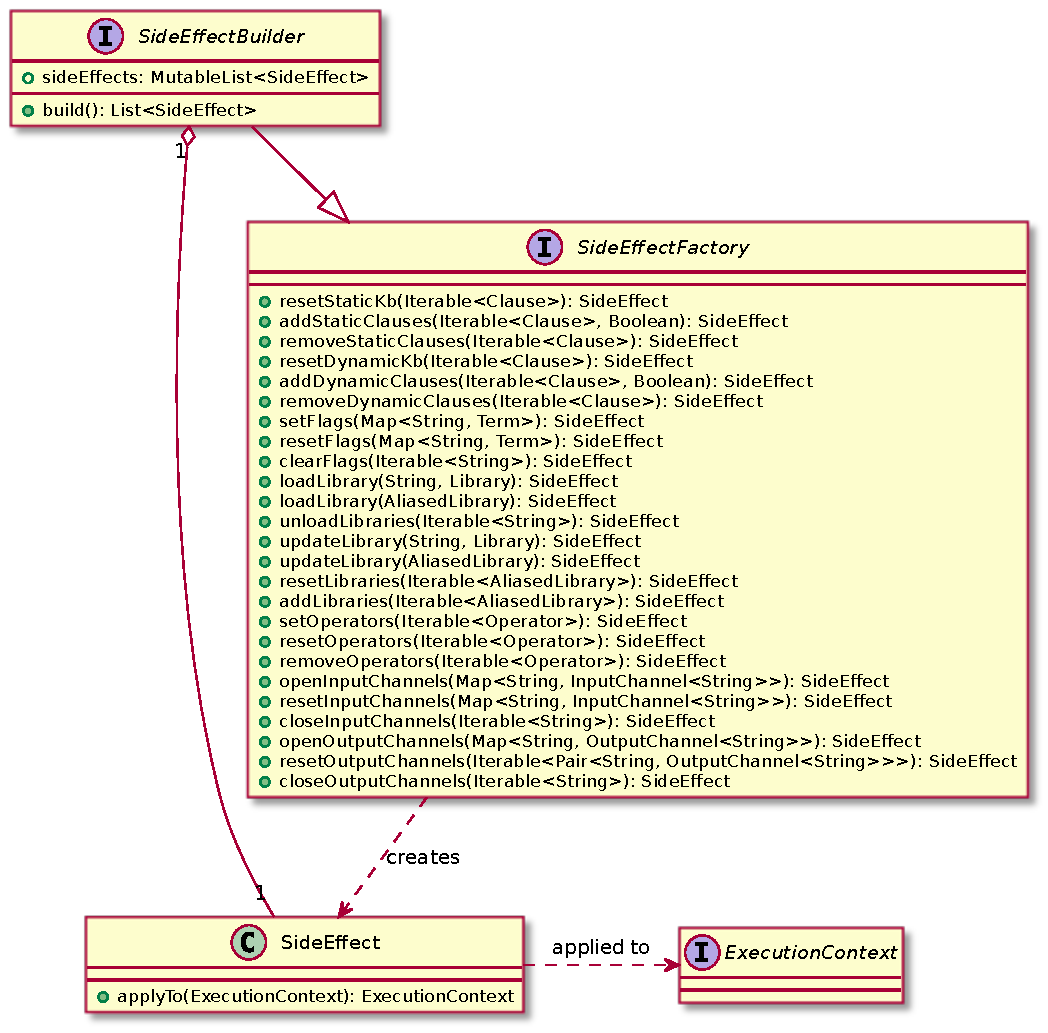
\includegraphics[height=.75\textheight]{img/sideeffects.pdf}
    \end{center}

    \begin{block}{\kt{SideEffect}s creation}
        \begin{itemize}
            \item Side effects are created along with \kt{Responses}
            \item \ldots via \kt{SideEffects\alert{Builder}}\alert{s}
            %
            \begin{itemize}
                \item overloads exist for each \kt{Response.\alert{reply*}} method
                \item supporting the syntax:
                %
                \begin{center}
                    \kt{request.reply*(solution) \alert{\{ \meta{add side effects here} \}}}
                \end{center}
            \end{itemize}
        \end{itemize}
    \end{block}

    \framebreak

    \ktSnippet{snippets/MissingExample.kt}
    % assert

\end{frame}

\begin{frame}[allowframebreaks]{The \kt{PrologFunction} Type}
    \begin{alertblock}{Problem}
        \begin{itemize}
            \item Some predicates may require \alert{logic expressions} to be \alert{evalued} / \alert{reduced}
            %
            \begin{itemize}
                \item[eg] \pl{X is Y + 1} (which is equal to \alert{\pl{is(X, '+'(Y, 1))}})
            \end{itemize}
            \item Evaluation may involve several \alert{functions}
            %
            \begin{itemize}
                \item[ie] objects consuming $N \geq$ terms a producing a \alert{result}
                %
                \begin{itemize}
                    \item which is, in turn, a \kt{Term}
                \end{itemize}
            \end{itemize}
            \item Plugging \alert{custom} functions into a \kt{Solver} should be possible
        \end{itemize}
    \end{alertblock}

    \begin{block}{Why \kt{PrologFunction}s}
        \begin{itemize}
            \item A means for calling Kotlin code from LP
            %
            \begin{itemize}
                \item with the purpose of \alert{evaluating} an expression
            \end{itemize}
        \end{itemize}
    \end{block}

    \framebreak

    Design very similar to \kt{Primitives}:
    %
    \begin{center}
        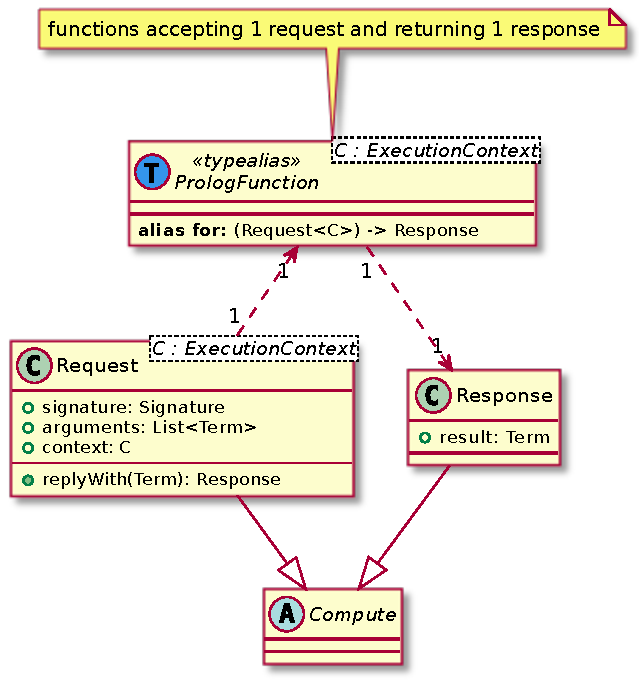
\includegraphics[height=.7\textheight]{img/function.pdf}
    \end{center}
    %
    \begin{itemize}
        \item[!] no support for side effects, nor multiple responses
    \end{itemize}

    \framebreak

    \ktSnippet{snippets/MissingExample.kt}
    % sum (functional)

    \framebreak

    \begin{alertblock}{About \kt{PrologFunction}s usage}
        Expression evaluation:
        % 
        \begin{itemize}
            \item is expected to \alert{only} occur as part of some \kt{Primitive} execution
            \item is likely to involve \alert{several} \kt{PrologFunction}s
            \item must be \alert{atomic} in the eyes of the \kt{Solver}
        \end{itemize}
    \end{alertblock}

    \begin{exampleblock}{Example: the \pl{is/2} predicate}
        \begin{itemize}
            \item Prolog's \pl{is/2} is both an operator and a primitive in \twopkt{}
            \item Whenever a goal of the form \pl{is(X, Expr)} is met:
            %
            \begin{itemize}
                \item \pl{Expr} is \alert{evalued}, by applying \alert{all} possible functions
                \item the resulting term is bound to \pl{X}
            \end{itemize}
        \end{itemize}
    \end{exampleblock}

    \framebreak

    \alert{Evaluators} aim to ``apply \alert{all possible} functions'' to an expression:
    %
    \begin{center}
        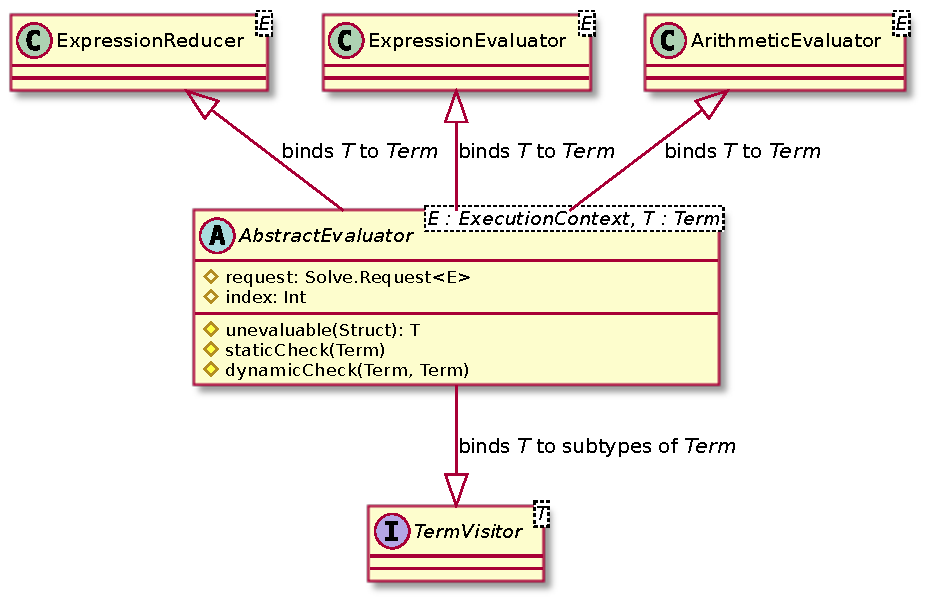
\includegraphics[width=.5\linewidth]{img/evaluator.pdf}
    \end{center}
    %
    \small
    where
    %
    \begin{itemize}
        \item ``all possible functions'' = \emph{``all functions currently loaded into the \kt{Solver}''}
    \end{itemize}

    \framebreak

    \begin{block}{Sorts of evaluators}
        \begin{description}
            \item[\kt{ExpressionReducer}] reduces all sub-expressions matching some function, leaving others unreduced
            %
            \begin{itemize}\small
                \item sub-expressions are evalued using a \alert{post-order} visit
                \item[eg] \pl{g(f(1 + 2), 3 + 4)} $\rightarrow$ \pl{g(f(3), 7)} 
            \end{itemize} 
            \item[\kt{ExpressionEvaluator}] attempts to evaluate all sub-expressions matching some function, throws an error if some does not
            %
            \begin{itemize}\small
                \item sub-expressions are evalued using a \alert{post-order} visit
                \item[eg] \pl{(1 + 2) - (3 + f(x))} $\rightarrow$ error as there is no function for \pl{f/1}
            \end{itemize} 
            \item[\kt{ArithmeticEvaluator}] like \kt{ExpressionEvaluator}, but only leverages on arithmetic functions
            %
            \begin{itemize}\small
                \item[ie] functions accepting and returning \kt{Numeric} arguments
            \end{itemize} 
        \end{description}
    \end{block}

    \framebreak

    \ktSnippet{snippets/MissingExample.kt}
    % implementation of the is/2 primitive
\end{frame}

\subsubsection{Communicating with the external world via \kt{Channel}s}

\begin{frame}[allowframebreaks]{Overview on \kt{Channel}s}
    \begin{block}{Why \kt{Channel}s}
        \begin{itemize}
            \item \kt{Solver}s are \alert{prosumers} of data \alert{streams}
            \item Data represented in the form of \alert{characters} / \alert{strings}
            \item I/O facilities similar to Java's \kt{Reader}s and \kt{Writer}s are needed
            %
            \begin{itemize}
                \item[!] unfortunately, Kotlin MP does not support I/O
            \end{itemize}
        \end{itemize}
    \end{block}

    \begin{block}{Design choices}
        \begin{itemize}
            \item \kt{Channel}s are of 2 sorts: either \kt{InputChannel}s or \kt{OutputChannel}s
            %
            \begin{itemize}
                \item \kt{InputChannel}s (aka \alert{sources}) let \kt{Solver}s read data of type \kt{T}
                \item \kt{OutputChannel}s (aka \alert{sinks}) let \kt{Solver}s write data of type \kt{T}
            \end{itemize}
            \item \kt{Channel}s are identified by univoke terms, in the eyes of \kt{Solver}s
            %
            \begin{itemize}
                \item or by some \alert{alias}, i.e. an \alert{atom}
            \end{itemize}
            \item \kt{Channel}s provide basic support to the features of \module{:io-lib}
            \item Each \kt{Solver} contains an \kt{InputStore} and an \kt{OutputStore}
            %
            \begin{itemize}
                \item keeping track of currently available \kt{Channel}s
                \item and their aliases
            \end{itemize}
        \end{itemize}
    \end{block}

    \begin{block}{Default \kt{Channel}s}
        Each \kt{Solver} is initialised with 4 default \kt{Channel}s:
        %
        \begin{description} 
            \item[\kt{stdIn: InputChannel<\textit{String}>}] main input channel
            \item[\kt{stdOut: OutputChannel<\textit{String}>}] main output channel 
            \item[\kt{stdErr: OutputChannel<\textit{String}>}] error channel
            \item[\kt{warnings: OutputChannel<\textit{PrologWarning}>}] warning channel 
            %
            \begin{itemize}
                \item does not output strings, but instances of \kt{PrologWarning}
            \end{itemize} 
        \end{description}
    \end{block}
\end{frame}

\begin{frame}[allowframebreaks]{The \kt{Channel} Type Hierarchy}
    \begin{center}
        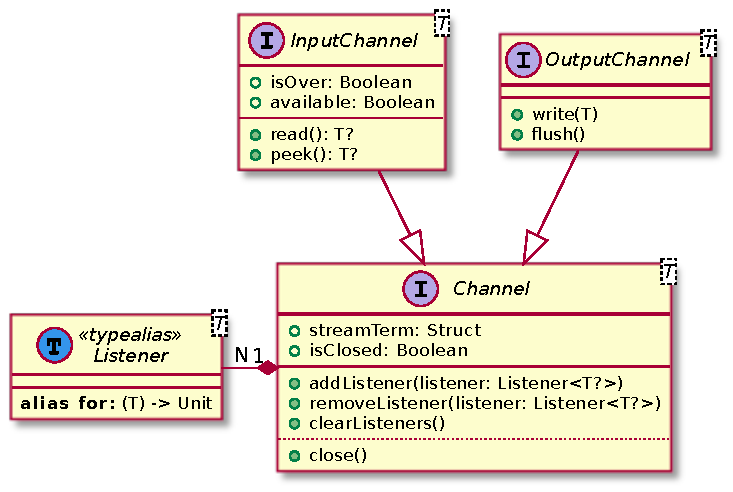
\includegraphics[width=.6\linewidth]{img/channels.pdf}
    \end{center}

    \begin{block}{The \kt{Channel<\texttt{T}>} type}\centering
        Base type for both input/output channels. 
        All channels are \alert{observable} entities supporting the (un)registration of \alert{listeners}.
    \end{block}
    %
    \begin{description}
        \item[\kt{addListener(Listener<T>)}] registers a new listener
        \item[\kt{removeListener(Listener<T>)}] unregisters a listener
        \item[\kt{clearListeners(Listener<T>)}] unregisters all listeners
        \item[\kt{close()}] closes the channel (no more write/read allowed)
        \item[\kt{isClosed: Boolean}] returns \kt{true} iff the channel has been closed
        \item[\kt{streamTerm: Struct}] returns the \kt{Struct} identifying this channel
        %
        \begin{itemize}\small
            \item is always a struct of the form:
            %
            \begin{center}
                \pl{'\$stream'(InOut, Id)}
            \end{center}
            where
            %
            \begin{itemize}\scriptsize
                \item \pl{InOut} is either \pl{`in'} or \pl{`out'}, depending on the sort of channel
                \item \pl{Id} is a number univokely identifying the channel instance
            \end{itemize}
        \end{itemize}  
    \end{description}

    \framebreak

    \begin{block}{The \kt{InputChannel<\texttt{T}>} type is a sub-type of \kt{Channel<\texttt{T}>}}\centering
        Base type for \alert{input} channels. 
        Support reading an instance of \kt{\texttt{T}} at a time, from some data source.
    \end{block}
    %
    \begin{description}
        \item[\kt{read(): T?}] consumes and returns the next instance of \kt{\texttt{T}} in the channel
        %
        \begin{itemize}\small
            \item returns \kt{null} if the channel is \alert{over}
            \item throws \kt{IllegalStateException} if the channel is \alert{closed}
        \end{itemize} 
        \item[\kt{peek(): T?}] like \kt{read}, but does not consume
        \item[\kt{available: Boolean}] returns \kt{true} iff  the next instance of \kt{\texttt{T}} can be read/peeked without blocking
        \item[\kt{isOver: Boolean}] returns \kt{tree} iff the next call to \kt{read}/\kt{peek} would return \kt{null}
    \end{description}

    \framebreak

    \begin{block}{The \kt{OutputChannel<\texttt{T}>} type is a sub-type of \kt{Channel<\texttt{T}>}}\centering
        Base type for \alert{output} channels. 
        Support writing an instance of \kt{\texttt{T}} at a time, onto some data sink.
    \end{block}
    %
    \begin{description}
        \item[\kt{write(T)}] writes an instance of \kt{\texttt{T}}
        %
        \begin{itemize}\small
            \item throws \kt{IllegalStateException} if the channel is \alert{closed}
        \end{itemize} 
        \item[\kt{flush()}] ensures data is actually written to the channel
        %
        \begin{itemize}\small
            \item (useful in case of buffering / caching)
        \end{itemize} 
    \end{description}

\end{frame}

\begin{frame}[allowframebreaks]{Creating \kt{Channel}s}

    \begin{block}{Design choices -- \kt{InputChannel}s}
        \kt{InputChannel}s may be created out of:
        %
        \begin{itemize}
            \item a \alert{generator} function (of type \alert{\kt{() -> T}})
            \item a \kt{String}---supporting its consumption \alert{character-wise}
            \item an \kt{InputStream} or \kt{Reader} (JVM only)
            %
            \begin{itemize}
                \item[eg] \kt{System.in}
            \end{itemize}
        \end{itemize}
    \end{block}
    %
    \begin{description}
        \item[\kt{stdIn(): InputChannel<String>}] returns a wrapper of the actual standard input of the current program
        %
        \begin{itemize}\small
            \item[eg] \kt{System.in} on the JVM
            \item[!] makes no sense on \alert{JS Browser-side} 
        \end{itemize} 
        \item[\kt{of(() -> \textit{T}): InputChannel<\textit{T}>}] creates an input channel out of a generator function
        \item[\kt{of(String): InputChannel<String>}] creates an input channel consuming a string \alert{character-wise}
    \end{description}

    \ktSnippet{snippets/MissingExample.kt}

    \framebreak

    \begin{block}{Design choices -- \kt{InputChannel}s}
        \kt{OutputChannel}s may be created out of:
        %
        \begin{itemize}
            \item a \alert{consumer} function (of type \alert{\kt{(T) -> Unit}})
            \item an \kt{OutputStream} or \kt{Writer} (JVM only)
            %
            \begin{itemize}
                \item[eg] \kt{System.out} or \kt{System.err}
            \end{itemize}
        \end{itemize}
    \end{block}
    %
    \begin{description}
        \item[\kt{stdOut(): OutputChannel<String>}] returns a wrapper of the actual standard output of the current program
        %
        \begin{itemize}\small
            \item[eg] \kt{System.out} on the JVM
            \item[eg] \kt{Console.log} on JS 
        \end{itemize}
        \item[\kt{stdErr(): OutputChannel<String>}] returns a wrapper of the actual standard error of the current program
        %
        \begin{itemize}\small
            \item[eg] \kt{System.err} on the JVM
            \item[eg] \kt{Console.error} on JS 
        \end{itemize} 
        \item[\kt{warn(): OutputChannel<PrologWarning>}] returns a channel outputting warnings to the actual standard error of the current program
        \item[\kt{of((\textit{T}) -> Unit): OutputChannel<\textit{T}>}] creates an output channel out of a consumer function
    \end{description}

    \ktSnippet{snippets/MissingExample.kt}
\end{frame}

\begin{frame}[allowframebreaks]{The \kt{ChannelStore} Type Hierarchy}

    \begin{center}
        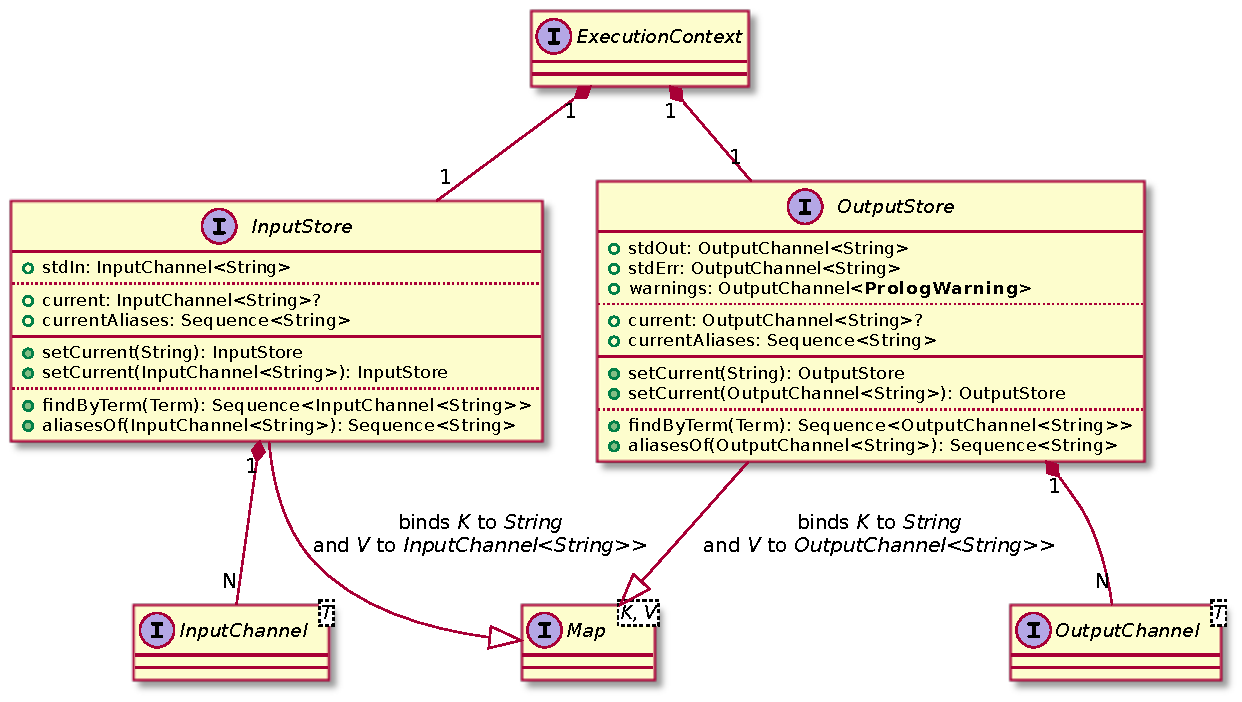
\includegraphics[width=.8\linewidth]{img/channels+stores.pdf}
    \end{center}

    \framebreak

    \begin{block}{The \kt{InputStore} type}
        Immmutable map keeping track of currently open \kt{InputChannel}s for a \kt{Solver}, and their aliases
        %
        \begin{itemize}
            \item References the \alert{standard} input channel
            \item Keeps track of the \alert{current} input channel
            %
            \begin{itemize}
                \item[ie] the one the \kt{Solver} reads from, by default
            \end{itemize}
        \end{itemize}
    \end{block}

    \framebreak

    \begin{block}{The \kt{OutputStore} type}
        Map keeping track of currently open \kt{OutputChannel}s for a \kt{Solver}, and their aliases
        %
        \begin{itemize}
            \item References the \alert{standard} input and error channels
            \item References the \alert{warnings} channel
            \item Keeps track of the \alert{current} output channel
            %
            \begin{itemize}
                \item[ie] the one the \kt{Solver} writes onto, by default
            \end{itemize}
        \end{itemize}
    \end{block}

    \framebreak

    Common methods:
    %
    \begin{description}
        \item[\kt{current: Channel<String>}] returns the current channel
        \item[\kt{setCurrent(Channel<String>)}] returns a new store having a different current channel
        \item[\kt{setCurrent(String)}] returns a new store having a different current channel (selected by \alert{alias})
        \item[\kt{findByTerm(Term)}] returns a channel by its identifier term
        \item[\kt{aliasesOf(Channel<String>)}] returns all the aliases of a given channel 
    \end{description}
    %
    \begin{itemize}
        \item[+] all methods of \kt{Map<String, Channel<String>>}
    \end{itemize}
\end{frame}

\begin{frame}[allowframebreaks]{Using \kt{Channel}s}
    \ktSnippet{snippets/MissingExample.kt}
    % creating solvers with custom channels

    \ktSnippet{snippets/MissingExample.kt}
    % attaching callbacks to a solver's channels
\end{frame}

\subsubsection{Configuring \kt{Solver}s via \kt{Flag}s}

\begin{frame}{Overview on flags}
    \begin{block}{About flags}
        \begin{itemize}
            \item Flags are key-value pairs carrying configurable aspects of \kt{Solver}s
            %
            \begin{itemize}
                \item \alert{keys} are \kt{String}s, whereas
                \item \alert{values} are \kt{Term}s
            \end{itemize}
            \item Some flags are editable, while others are \kt{read-only}
            %
            \begin{itemize}
                \item All flags can be inspected during resolution
                \item Editable flags' values can be altered during resolution
            \end{itemize}
            \item Custom flags may be defined/inspected during resultion
        \end{itemize}
    \end{block}
\end{frame}

\begin{frame}[allowframebreaks]{The \kt{FlagStore} and \kt{NotableFlag} Types}
    \begin{center}
        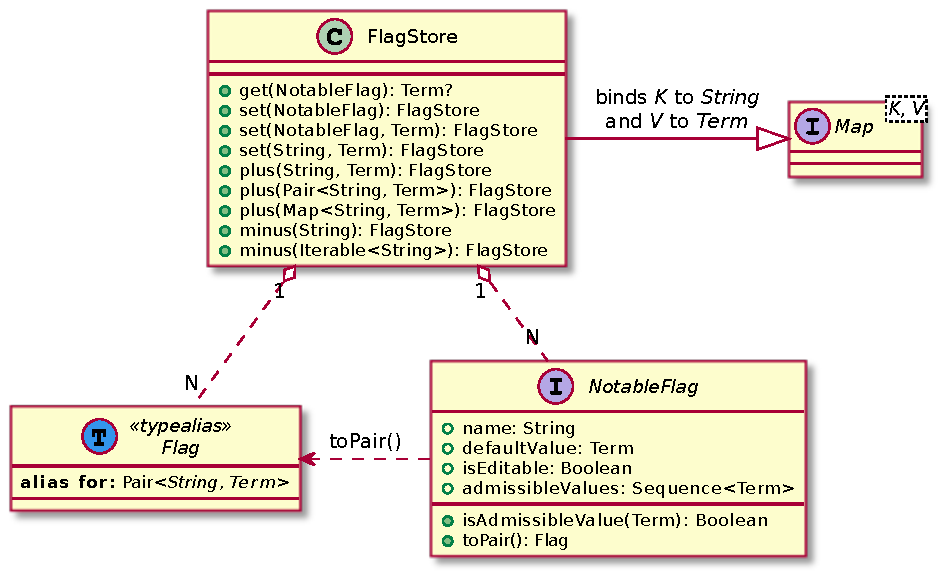
\includegraphics[width=.8\linewidth]{img/flags.pdf}
    \end{center}

    \begin{alertblock}{No type for flags}
        \begin{itemize}
            \item Kotlin's \kt{Pair}s are used instead
            \item Flag $\equiv$ \kt{Pair<String, Term>}, in the general case
            \item \kt{NotableFlag} as the convenience type for \alert{built-in} flags
        \end{itemize}
    \end{alertblock}

    \framebreak

    \begin{block}{The \kt{NotableFlag} type}\centering
        Ad-hoc type representing \alert{built-in} flags and their admissible values
    \end{block}
    %
    \begin{description}
        \item[\kt{name: String}] returns the name (i.e. the key) of the flag
        \item[\kt{admissibleValues: Sequence<Term>}] returns the set of admissible values of the flag
        \item[\kt{defaultValue: Term}] returns some item of \kt{admissibleValues}
        \item[\kt{isEditable: Boolean}] returns \kt{true} iff the flag's value can be altered during resolution
        \item[\kt{isAdmissibleValue(Term): Boolean}] checks whether the provided \kt{Term} is an admissible value for the flag
        \item[\kt{toPair(): Pair<String, Term>}] converts the notable flag into a key-value pair
    \end{description}

    \framebreak

    \begin{block}{The \kt{FlagStore} type}
        Immutable map keeping track of currently defined \alert{flags}' keys and their \alert{values}
        %
        \begin{itemize}
            \item[+] some methods for getting/setting \kt{NotableFlag}s
        \end{itemize}
    \end{block}
    %
    \begin{description}
        \item[\kt{get(NotableFlag): Term?}] returns the \emph{actual} value of some \alert{notable} flag 
        \item[\kt{get(String): Term?}] returns the \emph{actual} value of some flag
        \item[\kt{set(NotableFlag): FlagStore}] returns a novel store where the provided \alert{notable} flag is set to its \emph{default} value 
        \item[\kt{set(NotableFlag, Term): FlagStore}] returns a novel store where the provided \alert{notable} flag is set to the \emph{provided} value 
        \item[\kt{set(String, Term): FlagStore}] returns a novel store where the provided flag is set to the provided value 
        \item[\kt{plus(\meta{OtherFlags}): FlagStore}] returns a novel store containing the provided flags as well
        \item[\kt{minus(\meta{FlagNames}): FlagStore}] returns a novel store not containing the provided flags names 
    \end{description}
    %
    \begin{itemize}
        \item[+] methods of \kt{Map}
    \end{itemize}
\end{frame}

\begin{frame}[allowframebreaks]{Example: Default \kt{NotableFlag}s and their Purpose}

    \begin{block}{\pl{unknown}}
        Defines what to do when no rule/primitive is found for solving a (sub-)goal:
        %
        \begin{itemize}
            \item Class: \kt{it.unibo.tuprolog.solve.flags.\alert{Unknown}}
            \item Admissible values: 
            %
            \begin{description}
                \item[\pl{fail}] the goal is silently considered \pl{false}
                \item[\pl{warning}] \emph{(default)}  the goal is considered \pl{false} \& a warning is raised
                \item[\pl{error}] an error is raised and resolution is interrupted 
            \end{description}
        \end{itemize} 
    \end{block}

    \begin{block}{\pl{max\_arity}}
        Read-only flag dictating the maximum admissible value for a \kt{Struct}
        %
        \begin{itemize}
            \item Class: \kt{it.unibo.tuprolog.solve.flags.\alert{MaxArity}}
            \item Admissible values: \kt{Int.MAX\_VALUE} (i.e. $2^{31} - 1$)
        \end{itemize} 
    \end{block}

    \begin{block}{\pl{last\_call\_optimization}}
        Dictates whether Prolog \kt{Solver}s should optimise \alert{tail-recursive} rules
        %
        \begin{itemize}
            \item Class: \kt{it.unibo.tuprolog.solve.flags.\alert{LastCallOptimization}}
            \item Admissible values: 
            %
            \begin{description}
                \item[\pl{on}] \emph{(default)} optimization is performed whenever possible
                \item[\pl{off}] optimization is never perfomed
            \end{description}
        \end{itemize} 
    \end{block}

    \begin{block}{\pl{double\_quotes}}
        Read-only flag dictating how double-quoted literals should be interpreted
        %
        \begin{itemize}
            \item Class: \kt{it.unibo.tuprolog.solve.flags.\alert{DoubleQuotes}}
            \item Admissible values: \pl{atom}
            %
            \begin{itemize}
                \item[ie] double-quoted literals are always considered as \kt{Atom}
            \end{itemize}
        \end{itemize} 
    \end{block}
\end{frame}

\subsubsection{Other sorts of custom fields}

\begin{frame}[allowframebreaks]{Overview on \kt{CustomData}}

    \begin{center}
        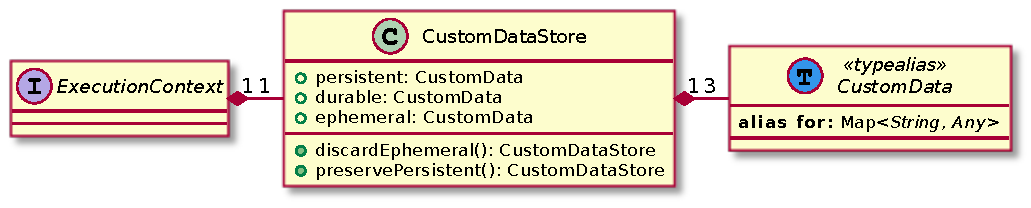
\includegraphics[width=.8\linewidth]{img/customdata.pdf}
    \end{center}
    
    \begin{block}{About \kt{CustomDataStore}s}
        \begin{itemize}
            \item To ease extensibility, \kt{ExecutionContext}s main contain \kt{CustomData} too
            \item This is acheieved via one more property, of type \kt{CustomDataStore}
            \item \kt{CustomDataStore}s have 3 fields of type \kt{CustomData}
            \item \kt{CustomData} are key-value store which may keep \alert{any sort} of data
            \item This may exploited by \kt{Primitive}s/\kt{Solver}s implementers
            %
            \begin{itemize}
                \item to accumulate/inspect data to affect resolution
            \end{itemize}
        \end{itemize}
    \end{block}

    \begin{block}{Sorts of \kt{CustomData}}
        Custom data are of 3 sorts:
        %
        \begin{description}
            \item[ephemeral] | automatically erased after a choice point is selected
            %
            \begin{itemize}\small
                \item[eg] in Prolog, once every time \alert{backtracking} is performed
            \end{itemize} 
            \item[durable] | automatically erased after a solution is reached
            \item[persistent] | never erased automatically
        \end{description}
    \end{block}
\end{frame}

\subsection{Errors and Warnings}

\begin{frame}[allowframebreaks]{The \kt{TuPrologRuntimeException} Type Hierarchy}
    
    \begin{center}
        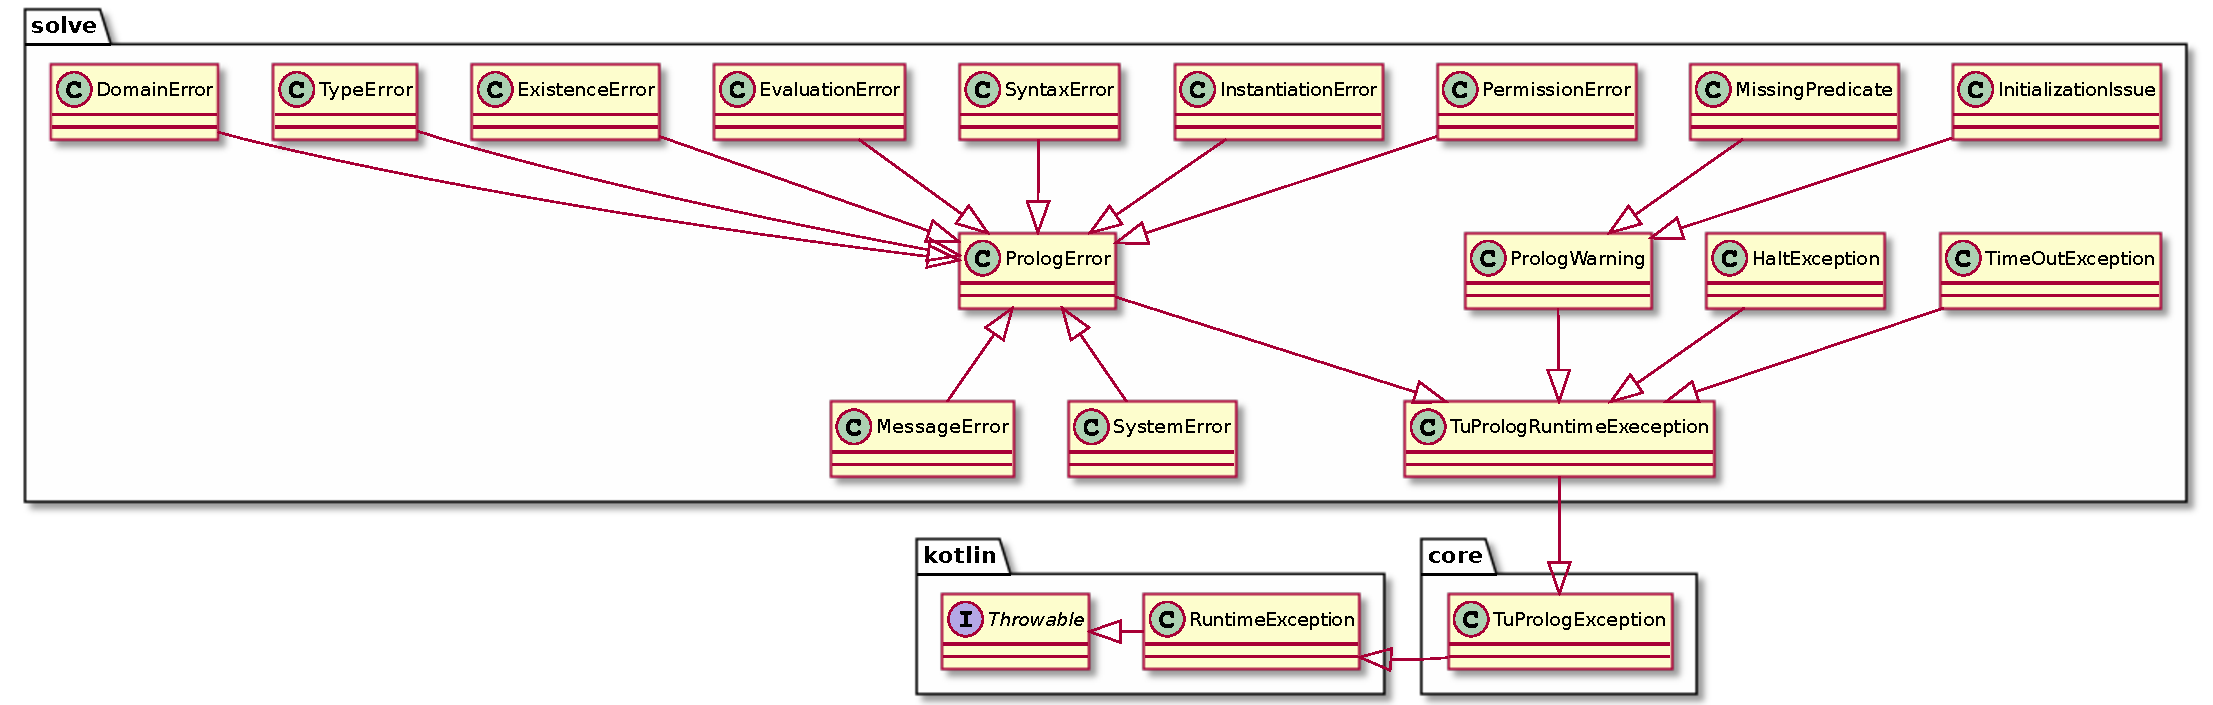
\includegraphics[width=\linewidth]{img/errors.pdf}
    \end{center}

    \framebreak

    \begin{description}
        \item[\kt{TuProlog\textit{Runtime}Exception}] base type for all issues which may occur during resolution 
        %
        \begin{itemize}\small
            \item when thrown \alert{within \kt{Primitive}s}, they affect the ongoing resolution
            \item resolution is interrupted, and a \kt{Solution.\alert{Halt}} is produced
            %
            \begin{itemize}\scriptsize
                \item the solution keeps track of the exception
                \item the exception keeps track of the execution context where the issue occurred
            \end{itemize}
        \end{itemize} 
         
        \item[\kt{HaltException}] provokes the immediate interruption of the resolution process
        %
        \begin{itemize}\small
            \item may carry an \alert{exit code} (integer)
            \item analogous to \kt{System.exit(\meta{int})} one the JVM
            \item produces a \kt{Solution.Halt}
        \end{itemize} 
        
        \item[\kt{TimeOutException}] provokes the immediate interruption of the resolution process
        %
        \begin{itemize}\small
            \item automatically thrown by \kt{Solver}s upon \alert{timeouts}
        \end{itemize}

        \framebreak
        
        \item[\kt{PrologError}] base types for LP-related errors
        %
        \begin{itemize}\small
            \item[ie] errors which can be catched in LP
            \item[eg] via \kt{catch/3}, in Prolog
        \end{itemize} 

        \item[\kt{PrologWarning}] base types for LP-related warnings
        %
        \begin{itemize}\small
            \item these are not meant to be thrown
            \item instances of \kt{PrologWarning} must be considered ordinary data structures to be outputted on the \kt{warnings} \kt{OutputChannel}
        \end{itemize} 
    \end{description}
\end{frame}

\begin{frame}[allowframebreaks]{The \kt{PrologError} Type Hierarchy}

    \begin{block}{About \kt{PrologError}s}
        \begin{itemize}
            \item Each instance of \kt{PrologError} corresponds to a \kt{Term}
            \item The term can be thrown with predicate \alert{\kt{throw/1}}\ldots
            \item \ldots and catched via \alert{\kt{catch/3}} 
        \end{itemize}
    \end{block}

    \begin{block}{Prolog ISO Standard Errors}
        Following the Standard:
        %
        \begin{itemize}
            \item each subtype of \kt{PrologError} has a corresponding \alert{error \kt{Struct}}
            \item the general pattern is as follows:
            %
            \begin{center}
                \pl{error(\textit{Description}, \textit{Custom})}
            \end{center}
            %
            where:
            %
            \begin{description}\small
                \item[\pl{\textit{Description}}] is a \kt{Term} whose structure depends on the particular sub-type of \kt{PrologError}
                %
                \begin{itemize}\scriptsize
                    \item it aims at describing the error, logically
                \end{itemize} 
                \item[\pl{\textit{Custom}}] is a custom, implementation-specific \kt{Term}
                %
                \begin{itemize}\scriptsize
                    \item \twopkt{}'s convention: it carries the message to be shown to the user
                    \item so, it is commonly an \kt{Atom}
                \end{itemize}  
            \end{description}
        \end{itemize}
    \end{block}

    \begin{description}
        \item[\kt{InstantiationError}] to be thrown when a sub-goal/argument is being evalued but it is not sufficiently instantiated
        %
        \begin{description}\small
            \item[\pl{\textit{Description}}] is always the atom \alert{\pl{instantiation\_error}}
            \item[\pl{\textit{Custom}}] describes what argument/sub-term provoked the error
        \end{description} 

        \framebreak

        \item[\kt{TypeError}] to be thrown when a sub-goal/argument is being evalued but has not the right logic type
        %
        \begin{description}\small
            \item[\pl{\textit{Description}}] is a \kt{Struct} of the form \pl{type\_error(\textit{Expected}, \textit{Culprit})}
            \item[\pl{\textit{Expected}}] is an \kt{Atom} describing the expected type
            %
            \begin{itemize}\scriptsize
                \item admissible values are contained into the class \kt{TypeError.\alert{Expected}}
                \item[eg] \pl{atom}, \pl{atomic}, \pl{callable}, \pl{character}, \pl{compound}, etc. 
            \end{itemize} 
            \item[\pl{\textit{Culprit}}] is the \kt{Term} having the wrong type
        \end{description} 

        \framebreak

        \item[\kt{DomainError}] to be thrown when a sub-goal/argument is being evalued and it has the right type, but its value is not admissible
        %
        \begin{description}\small
            \item[\pl{\textit{Description}}] is a \kt{Struct} of the form \pl{domain\_error(\textit{Expected}, \textit{Culprit})}
            \item[\pl{\textit{Expected}}] is an \kt{Atom} describing the expected value
            %
            \begin{itemize}\scriptsize
                \item admissible values are contained into the class \kt{DomainError.\alert{Expected}}
                \item[eg] \pl{not\_less\_than\_zero}, \pl{non\_empty\_list}, \pl{operator\_specifier}, etc. 
            \end{itemize} 
            \item[\pl{\textit{Culprit}}] is the \kt{Term} having the wrong value
        \end{description} 

        \framebreak

        \item[\kt{RepresentationError}] to be thrown when a value cannot be represented as a \kt{Term}
        %
        \begin{description}\small
            \item[\pl{\textit{Description}}] is a \kt{Struct} of the form \pl{representation\_error(\textit{Limit})}
            \item[\pl{\textit{Limit}}] describes the representation limit which has been hit
            %
            \begin{itemize}\scriptsize
                \item admissible values are contained into the class \kt{RepresentationError.\alert{Limit}}
                \item[eg] \pl{character}, \pl{character\_code}, \pl{max\_arity}, etc. 
            \end{itemize} 
        \end{description} 

        \framebreak

        \item[\kt{SyntaxError}] to be thrown when parsing some badly formed string during resolution
        %
        \begin{description}\small
            \item[\pl{\textit{Description}}] is always the atom \alert{\pl{syntax\_error}}
            \item[\pl{\textit{Custom}}] describes why the string could not be parsed, and localizes the issue into the string
        \end{description} 

        \framebreak

        \item[\kt{EvaluationError}] to be thrown when some expression evaluation meets an arithmetic issue
        %
        \begin{description}\small
            \item[\pl{\textit{Description}}] is a \kt{Struct} of the form \pl{evaluation\_error(\textit{Type})}
            \item[\pl{\textit{Type}}] describes the evaluation issue which has been met
            %
            \begin{itemize}\scriptsize
                \item admissible values are contained into the class \kt{EvaluationError.\alert{Type}}
                \item[eg] \pl{zero\_divisor}, \pl{int\_overflow}, \pl{float\_overflow}, etc. 
            \end{itemize} 
        \end{description} 

        \framebreak

        \item[\kt{ExistenceError}] to be thrown accessing some resource by name/reference fails because the resource does not exist 
        %
        \begin{description}\small
            \item[\pl{\textit{Description}}] is a \kt{Struct} of the form \pl{existence\_error(\textit{ObjectType}, \textit{Culprit})}
            \item[\pl{\textit{ObjectType}}] describes the sort of resource which does not exist
            %
            \begin{itemize}\scriptsize
                \item admissible values are contained into the class \kt{ExistenceError.\alert{ObjectType}}
                \item[eg] \pl{procedure}, \pl{source\_sink}, \pl{stream}, etc. 
            \end{itemize} 
        \end{description} 

        \framebreak

        \item[\kt{PermissionError}] to be thrown when performing an operation which is not permitted
        %
        \begin{description}\small
            \item[\pl{\textit{Description}}] is a \kt{Struct} of the form \pl{permission\_error(\textit{Operation}, \textit{Permission}, \textit{Culprit})}
            \item[\pl{\textit{Operation}}] describes the sort of operation which failed
            %
            \begin{itemize}\scriptsize
                \item admissible values are contained into the class \kt{PermissionError.\alert{Operation}}
                \item[eg] \pl{access}, \pl{invoke}, \pl{modify}, \pl{open}, etc. 
            \end{itemize} 
            \item[\pl{\textit{Permission}}] describes the sort of resource for which the operation is not permitted
            %
            \begin{itemize}\scriptsize
                \item admissible values are contained into the class \kt{PermissionError.\alert{Permission}}
                \item[eg] \pl{flag}, \pl{operator}, \pl{source\_sink}, \pl{static\_procedure}, etc. 
            \end{itemize} 
            \item[\pl{\textit{Culprit}}] is the (sub-)goal which provoked the error
        \end{description} 

        \framebreak

        \item[\kt{SystemError}] to be thrown for any other circumstance
        %
        \begin{description}\small
            \item[\pl{\textit{Description}}] is always the atom \alert{\pl{system\_error}}
            \item[\pl{\textit{Custom}}] provides the actual description of the problem
        \end{description} 
        %
        \begin{itemize}
            \item[!] this may be used to wrap Kotlin exceptions occurring during resolution
        \end{itemize}
    \end{description} 
\end{frame}

\begin{frame}{The \kt{PrologWarning} Type Hierarchy}

    Main sub-types:
    %
    \bigskip
    %
    \begin{description}
        \item[\kt{MissingPredicate}] used to signal that a \kt{Solver} knows no predicate to solve a (sub-)goal
        
        \bigskip

        \item[\kt{InitializationIssue}] used to signal a failure/error while executing some \alert{directive}
    \end{description}
\end{frame}

\subsection{Custom \kt{Primitive}s, \kt{Function}s, and \kt{Libraries}s}

\begin{frame}[allowframebreaks]{Overview on Custom Libraries}
    containers of operators + rules + primitives + functions

    aliased by a string

    they take priority over solvers KB

    primitives as the main way to implement back-trackable predicates in Kotlin

    primitives as the main way to implement logic functions in Kotlin
\end{frame}

\subsubsection{About \kt{PrimitiveWrappers} and \kt{SideEffect}s}

\begin{frame}[allowframebreaks]{Overview on \kt{PrimitiveWrappers}}
    enumerate the sorts of primitive wrappers

    description of the general Pattern

    list of ensurer methods
\end{frame}

\begin{frame}[allowframebreaks]{Example of \kt{PrimitiveWrappers} of all sorts}
   one example for each sort of primitive wrapper from the CommonBuiltins
\end{frame}

\subsubsection{Writing \kt{Library}}

\begin{frame}[allowframebreaks]{\kt{Library} end-to-end}
    full example of a library containing at least 1 operator, 1 rule, 1 primitive and 1 function

    loading the library into a solver
 \end{frame}

\subsubsection{Default libraries}

\begin{frame}[allowframebreaks]{Example: The \kt{CommonBuiltins} Type}
    which items does it include and what's their type, and why

    example of rule

    example of primitive

    example of function
\end{frame}

\section{Prolog as a State Machine: the \module{solve-classic} Module}

\begin{frame}[allowframebreaks]{Overview on the \module{solve-classic} Module}
    state machine based design

    AbstractClassicSolver

    SolutionIterator

    ClassicSolver
\end{frame}

\begin{frame}[allowframebreaks]{Formal State Machine}
    whole formalization here
\end{frame}

\begin{frame}[allowframebreaks]{State Machine in Practice}
    design of state

    responsibilities of each state

    iterating over states
\end{frame}

\section{Reading and Writing Data: the \module{io-lib} Module}

\begin{frame}[allowframebreaks]{Overview on IO in LP}
    urls for locating resources

    sinks and sources

    main predicates
\end{frame}

\begin{frame}[allowframebreaks]{Platform-specific Issues}

\end{frame}

\section{OOP and Prolog: the \module{oop-lib} Module}

\begin{frame}[allowframebreaks]{Overview on the OOP Lib Design}
    references to types and objects

    term to object conversions
        + smart cast and overloading selection

    object to term conversions

    ad-hoc predicates

    ad-hoc operators

    aliases
\end{frame}

\subsection{\kt{Ref}erences: \kt{TypeRef}erences and \kt{ObjectRef}}

\begin{frame}[allowframebreaks]{The \kt{Ref} Type Hierarchy}
    definition and API of ref

    definition and API of object ref

    definition and API of null ref

    definition and API of type ref
\end{frame}

\begin{frame}[allowframebreaks]{Creation of \kt{Ref}erences}
    static factories for refs

    type factories
\end{frame}

\subsection{OOP to/from LP Conversions}

\begin{frame}[allowframebreaks]{The \kt{TermToObjectConverter} Type}
    definition

    api

    implemented strategy

    example
\end{frame}

\begin{frame}[allowframebreaks]{The \kt{ObjectToTermConverter} Type}
    definition

    api

    implemented strategy

    example
\end{frame}

\subsection{Overload Selection}

\begin{frame}[allowframebreaks]{The \kt{OverloadSelector} Type}
    definition

    api

    implemented strategy

    example
\end{frame}

\subsection{Logic Predicates and Operators for OOP}

\begin{frame}[allowframebreaks]{Main Predicates from the OOP Lib}
    (for each: definition, semantics)

    \ttfamily
    invoke\_method/3
    invoke\_strict/3
    assign/3
    cast/3
    new\_object/3
    new\_object/2 (rule)
    register/2
    unregister/1
    alias/2 (rule)
    :=/2 (rule)
    ./2 (rule)
    fluent\_reduce/3
    property\_reduce/3
\end{frame}

\section{LP + OOP + FP in Kotlin: the \module{dsl-*} Modules}

\begin{frame}[allowframebreaks]{Overview on the DSL}
    purpose

    principles (from \cite{kotlinDSl4PrologWoa2020})

    organization
\end{frame}

\begin{frame}[allowframebreaks]{Architecture}
    class diagram
\end{frame}

\begin{frame}[allowframebreaks]{Usage Example}
    reuse examples from \cite{kotlinDSl4PrologWoa2020}
\end{frame}

\section{Parsing Logic Knowledge: the \module{parser-*} Modules}

\begin{frame}[allowframebreaks]{The \kt{TermParser} Type}
    definition

    creation

    usage examples
\end{frame}

\begin{frame}[allowframebreaks]{The \kt{TermReader} Type (JVM-only)}
    definition

    creation

    usage examples
\end{frame}

\begin{frame}[allowframebreaks]{The \kt{ClausesParser} Type}
    definition

    creation

    usage examples
\end{frame}

\section{(De)Serialising Logic Knowledge: the \module{serialize-*} Modules}

\begin{frame}[allowframebreaks]{(De)Serialisation Overview}
    onion design: (de)objectifiers <-> (de)serializers

    single/multiple design: core vs. theory

    supported mime types: json and yaml
\end{frame}

\begin{frame}[allowframebreaks]{The \kt{TermSerializer} Type}
    definition

    creation
\end{frame}

\begin{frame}[allowframebreaks]{The \kt{TermDeserializer} Type}
    definition

    creation
\end{frame}

\begin{frame}[allowframebreaks]{The \kt{TheorySerializer} Type}
    definition

    creation
\end{frame}

\begin{frame}[allowframebreaks]{The \kt{TheoryDeserializer} Type}
    definition

    creation
\end{frame}

\begin{frame}[allowframebreaks]{Terms/Thoery to JSON Mapping}
    mapping definition
\end{frame}

\begin{frame}[allowframebreaks]{Complete Usage Example}
    serialize-and-then-deserialize example
\end{frame}

\section{Using \twopkt}

\subsection{As a library, for developers}

\subsubsection{For Java Developers}

\begin{frame}[allowframebreaks]{How to call Kotlin from Java}
    notable aspects
\end{frame}

\subsubsection{For JavaScript Developers}

\begin{frame}[allowframebreaks]{How to call Kotlin from JavaScript}
    notable aspects
\end{frame}

\subsection{As an application, for end users}

\subsubsection{Graphical User Interface: the \module{ide} Module}

\begin{frame}[allowframebreaks]{Usage of the IDE}
    how to launch the gui

    how to use the gui
\end{frame}

\subsubsection{Command Line Interface: the \module{cli} Module}

\begin{frame}[allowframebreaks]{Usage of the CLI}
    how to launch the cli
        + cli arguments

    how to use the cli
\end{frame}

\section*{}
\frame{\titlepage}

\section*{\bibname}

\setbeamertemplate{page number in head/foot}{}

\begin{frame}[t,allowframebreaks,noframenumbering]\frametitle{\refname}
% \begin{frame}[c]\frametitle{\refname}
    \footnotesize
%    \scriptsize
    \bibliographystyle{plain}
    \bibliography{2p-kt-talk}
\end{frame}

%%%%%%%%%%%%%%%%%%%%%%%%%%%%%%%%%%%%%%%%%%%%%%%%%%%%%%%%%%%%%%%%%%%%%%%%%%%%%%%%
\end{document}
%%%%%%%%%%%%%%%%%%%%%%%%%%%%%%%%%%%%%%%%%%%%%%%%%%%%%%%%%%%%%%%%%%%%%%%%%%%%%%%%
